\documentclass[11pt]{article}

\usepackage[a4paper,margin=1.5in]{geometry}
\usepackage[strict]{changepage}
\usepackage[scale=0.92]{tgschola}
\usepackage{fouriernc}
\usepackage[T1]{fontenc}

\usepackage{booktabs, threeparttable, adjustbox, tabularx, longtable}
\usepackage{amsmath, amssymb, amsthm, bbm}
\usepackage{hyperref, achicago}
\usepackage{caption, graphicx}
\usepackage{secdot, sectsty}
\usepackage{pdflscape}
\usepackage{placeins}
\usepackage{xcolor}

\fontfamily{qcs}
\linespread{1.1}
\urlstyle{tt}

\allsectionsfont{\rmfamily}
\sectionfont{\normalsize}
\subsectionfont{\normalsize\selectfont}
\subsubsectionfont{\normalfont\normalsize\selectfont\itshape}

\newcommand{\specialcell}[2][c]{\begin{tabular}[#1]{@{}c@{}}#2\end{tabular}}
\renewcommand{\today}{\ifcase \month \or January \or February \or March \or April \or May  \or June \or July \or August \or September \or October \or November \or December \fi~\number \year}

\begin{document}

\title{\textsc{Using Lotteries to Encourage Saving: Appendix}\protect\footnote{For online publication only. Files for replication are available at \url{https://github.com/princetonbpl/akiba-lottery-pub}.}}

\author{Justin Abraham\thanks{Department of Economics. University of California, San Diego. \protect\href{mailto:jabraham@ucsd.edu}{\nolinkurl{jabraham@ucsd.edu}}.}, Merve Akbas\thanks{Department of Economics. Duke University. \protect\href{mailto:merve.akbas@duke.edu}{\nolinkurl{merve.akbas@duke.edu}}.}, Dan Ariely\thanks{Fuqua School of Business. Duke University. \protect\href{mailto:dan@danariely.com}{\nolinkurl{dan@danariely.com}}.}, and Chaning Jang\thanks{The Busara Center for Behavioral Economics. \protect\href{mailto:chaning.jang@busaracenter.org}{\nolinkurl{chaning.jang@busaracenter.org}}.}} % add funding statement and ethics and thanks

\maketitle

\newpage

\tableofcontents

\newpage

\appendix

\section{Experimental Materials}

    \subsection{Consent form}

        {\setlength{\parskip}{1em} \setlength{\parindent}{0em}

        You are asked to participate in research project conducted by researchers at Duke University, Dan Ariely (dan@danariely.com) and Seher Merve Akbas (merve.akbas@duke.edu). The purpose of this project is (1) to understand how people make decisions about money, (2) how people make risky decisions, (3) how people decide to save money.

        During the study in the laboratory, you will be presented a number of decisions involving money. Your payment will depend on your decisions and specific rules about it will be explained to you before you start.

        Your participation in this project is completely voluntary and you are free to withdraw from it at any time. During the project, all the information about you will be analyzed anonymously and reported by groups.

        Do you have any questions that you would like to ask now?

        For any future questions or concerns about the project, please contact the researcher Seher Merve Akbas via e-mail (merve.akbas@duke.edu) or phone (+1919-328-0080) or Dan Ariely via e-mail (dan@danariely.com) or the project associate, James Vancel (email: jvancel@poverty-action.org) (Phone: +254725066428), or the project manager, Joseph Njoroge (jmuiruri@poverty-action.org) (Phone: +254722900068).

        I have read this information, and would like to participate

        Name: \qquad Date:

        }

    \subsection{Savings account}

        \subsubsection{Account instructions (Control)}

            {\setlength{\parskip}{1em} \setlength{\parindent}{0em}

            Here, we are introducing you AKIBA SMART, which will allow you to save money for a period of four weeks (28 days). Now I will explain how AKIBA SMART works. Using AKIBA SMART, you can save money by sending airtime (via Sambaza) to 0726-085246. The net worth of the airtime you send will be the amount you save. For example, if you send Airtime worth 20KSh it means you saved 20Ksh. This way, you won't pay any MPESA fees to save.

            AKIBA SMART helps you save in two ways:

            1. Every day, AKIBA SMART will add 5\% of your daily savings to your account. For example, if you saved 20KSH, you will receive 1 KSH extra. The more you save each day, the more money you will accumulate yourself. Furthermore, the more you save, the more you will receive extra from AKIBA SMART.

            2. You will be able to keep your money in a safe place for 28 days, and at the end of 28 days, you will receive all your savings, with the extra money you received from AKIBA SMART back via MPESA (you won't receive Airtime).

            As a promotion, you are automatically enrolled in AKIBA SMART today. You will receive your ID cards now and you can start saving immediately. [We will try out how it works here. As part of our promotion, we will give you some money to save today to learn how it works. This money is yours and you will receive it at the end of 28 days.]

            Do you have any questions?

            }

        \subsubsection{Account instructions (Lottery)}

            {\setlength{\parskip}{1em} \setlength{\parindent}{0em}

            Here, we are introducing you AKIBA SMART, which will allow you to save money for a period of four weeks (28 days). Now I will explain how AKIBA SMART works. Using AKIBA SMART, you can save money by sending airtime (via Sambaza) to 0726-085246. The net worth of the airtime you send will be the amount you save. For example, if you send Airtime worth 20KSh it means you saved 20Ksh. This way, you won't pay any MPESA fees to save.

            AKIBA SMART helps you save in two ways:

            1. Every day, if you save, you will receive your Lottery Ticket in an SMS and you will enter a lottery. The next day, you will be notified by SMS whether you won, and how much money you won. If you win, the prize will be added to your account. If you don't win, you will still keep your savings. This will continue every day for 28 days. The more you save each day, the more money you will accumulate yourself. Furthermore, the more you save, the bigger the prizes!!!

            2. You will be able to keep your money in a safe place for 28 days, and at the end of 28 days you will receive all your savings, with the prizes you won back via MPESA (you won't receive Airtime).

            The lottery works as follows:

            Each day, if you save, you will receive a lottery ticket as SMS. The lottery ticket includes 4 numbers between 1 and 10. If the FIRST OR SECOND number in your lottery ticket match the first or second number in the winning ticket, you win Prize 1: 10\% of what you saved that day! For example, if you saved 20KSH that day, you win 2 KSH extra. If the FIRST AND SECOND numbers in your lottery ticket match the first and second numbers in the winning ticket, you win Prize 2: 100\% of what you saved that day! For example, if you saved 20KSH that day, you win 20 KSH extra. If the ALL NUMBERS in your lottery ticket match all numbers in the winning ticket in the same order, you win Prize 3: 200 times what you saved that day! For example, if you saved 20KSH that day, you win 4000 KSH extra.

            As a promotion, you are automatically enrolled in AKIBA SMART today. You will receive your ID cards now and you can start saving immediately. [We will try out how it works here. As part of our promotion, we will give you some money to save today to learn how it works. This money is yours and you will receive it at the end of 28 days.]

            Do you have any questions?

            }

        \subsubsection{Account instructions (Regret)}

            {\setlength{\parskip}{1em} \setlength{\parindent}{0em}

            Here, we are introducing you AKIBA SMART, which will allow you to save money for a period of four weeks (28 days). Now I will explain how AKIBA SMART works.
            Using AKIBA SMART, you can save money by sending airtime (via Sambaza) to 0726-085246. The net worth of the airtime you send will be the amount you save. For example, if you send Airtime worth 20KSh it means you saved 20Ksh. This way, you won't pay any MPESA fees to save.

            AKIBA SMART helps you save in two ways:

            1. Every day, you will receive your Lottery Ticket in an SMS and you will enter a lottery. The next day, you will be notified by SMS whether you won, and how much money you won. If you win, your prize will be added to your account ONLY IF YOU SAVED that day, if you did not save, you will give up your prize. If you don't win, you will still keep your savings. This will continue every day for 28 days. The more you save each day, the more money you will accumulate yourself. Furthermore, the more you save, the bigger the prizes!!!

            2. You will be able to keep your money in a safe place for 28 days, and at the end of 28 days you will receive all your savings, with the prizes you won back via MPESA (you won't receive Airtime).

            The lottery works as follows:

            Each day, you will receive a lottery ticket as SMS. The lottery ticket includes 4 numbers between 1 and 10. If the FIRST OR SECOND number in your lottery ticket match the first or second number in the winning ticket, you win Prize 1: 10\% of what you saved that day! For example, if you saved 20KSH that day, you win 2 KSH extra. If the FIRST AND SECOND numbers in your lottery ticket match the first and second numbers in the winning ticket, you win Prize 2: 100\% of what you saved that day! For example, if you saved 20KSH that day, you win 20 KSH extra. If the ALL NUMBERS in your lottery ticket match all numbers in the winning ticket in the same order, you win Prize 3: 200times what you saved that day! For example, if you saved 20KSH that day, you win 4000 KSH extra.

            REMEMBER: YOU CAN REDEEM YOUR PRIZE ONLY IF YOU SAVED THAT DAY.

            As a promotion, you are automatically enrolled in AKIBA SMART today. You will receive your ID cards now and you can start saving immediately. [We will try out how it works here. As part of our promotion, we will give you some money to save today to learn how it works. This money is yours and you will receive it at the end of 28 days.]

            Do you have any questions?

            }

        \clearpage

        \begin{figure}[ht]
        \caption{Savings ID cards}
        \centering
        \begin{tabular}{cc}
        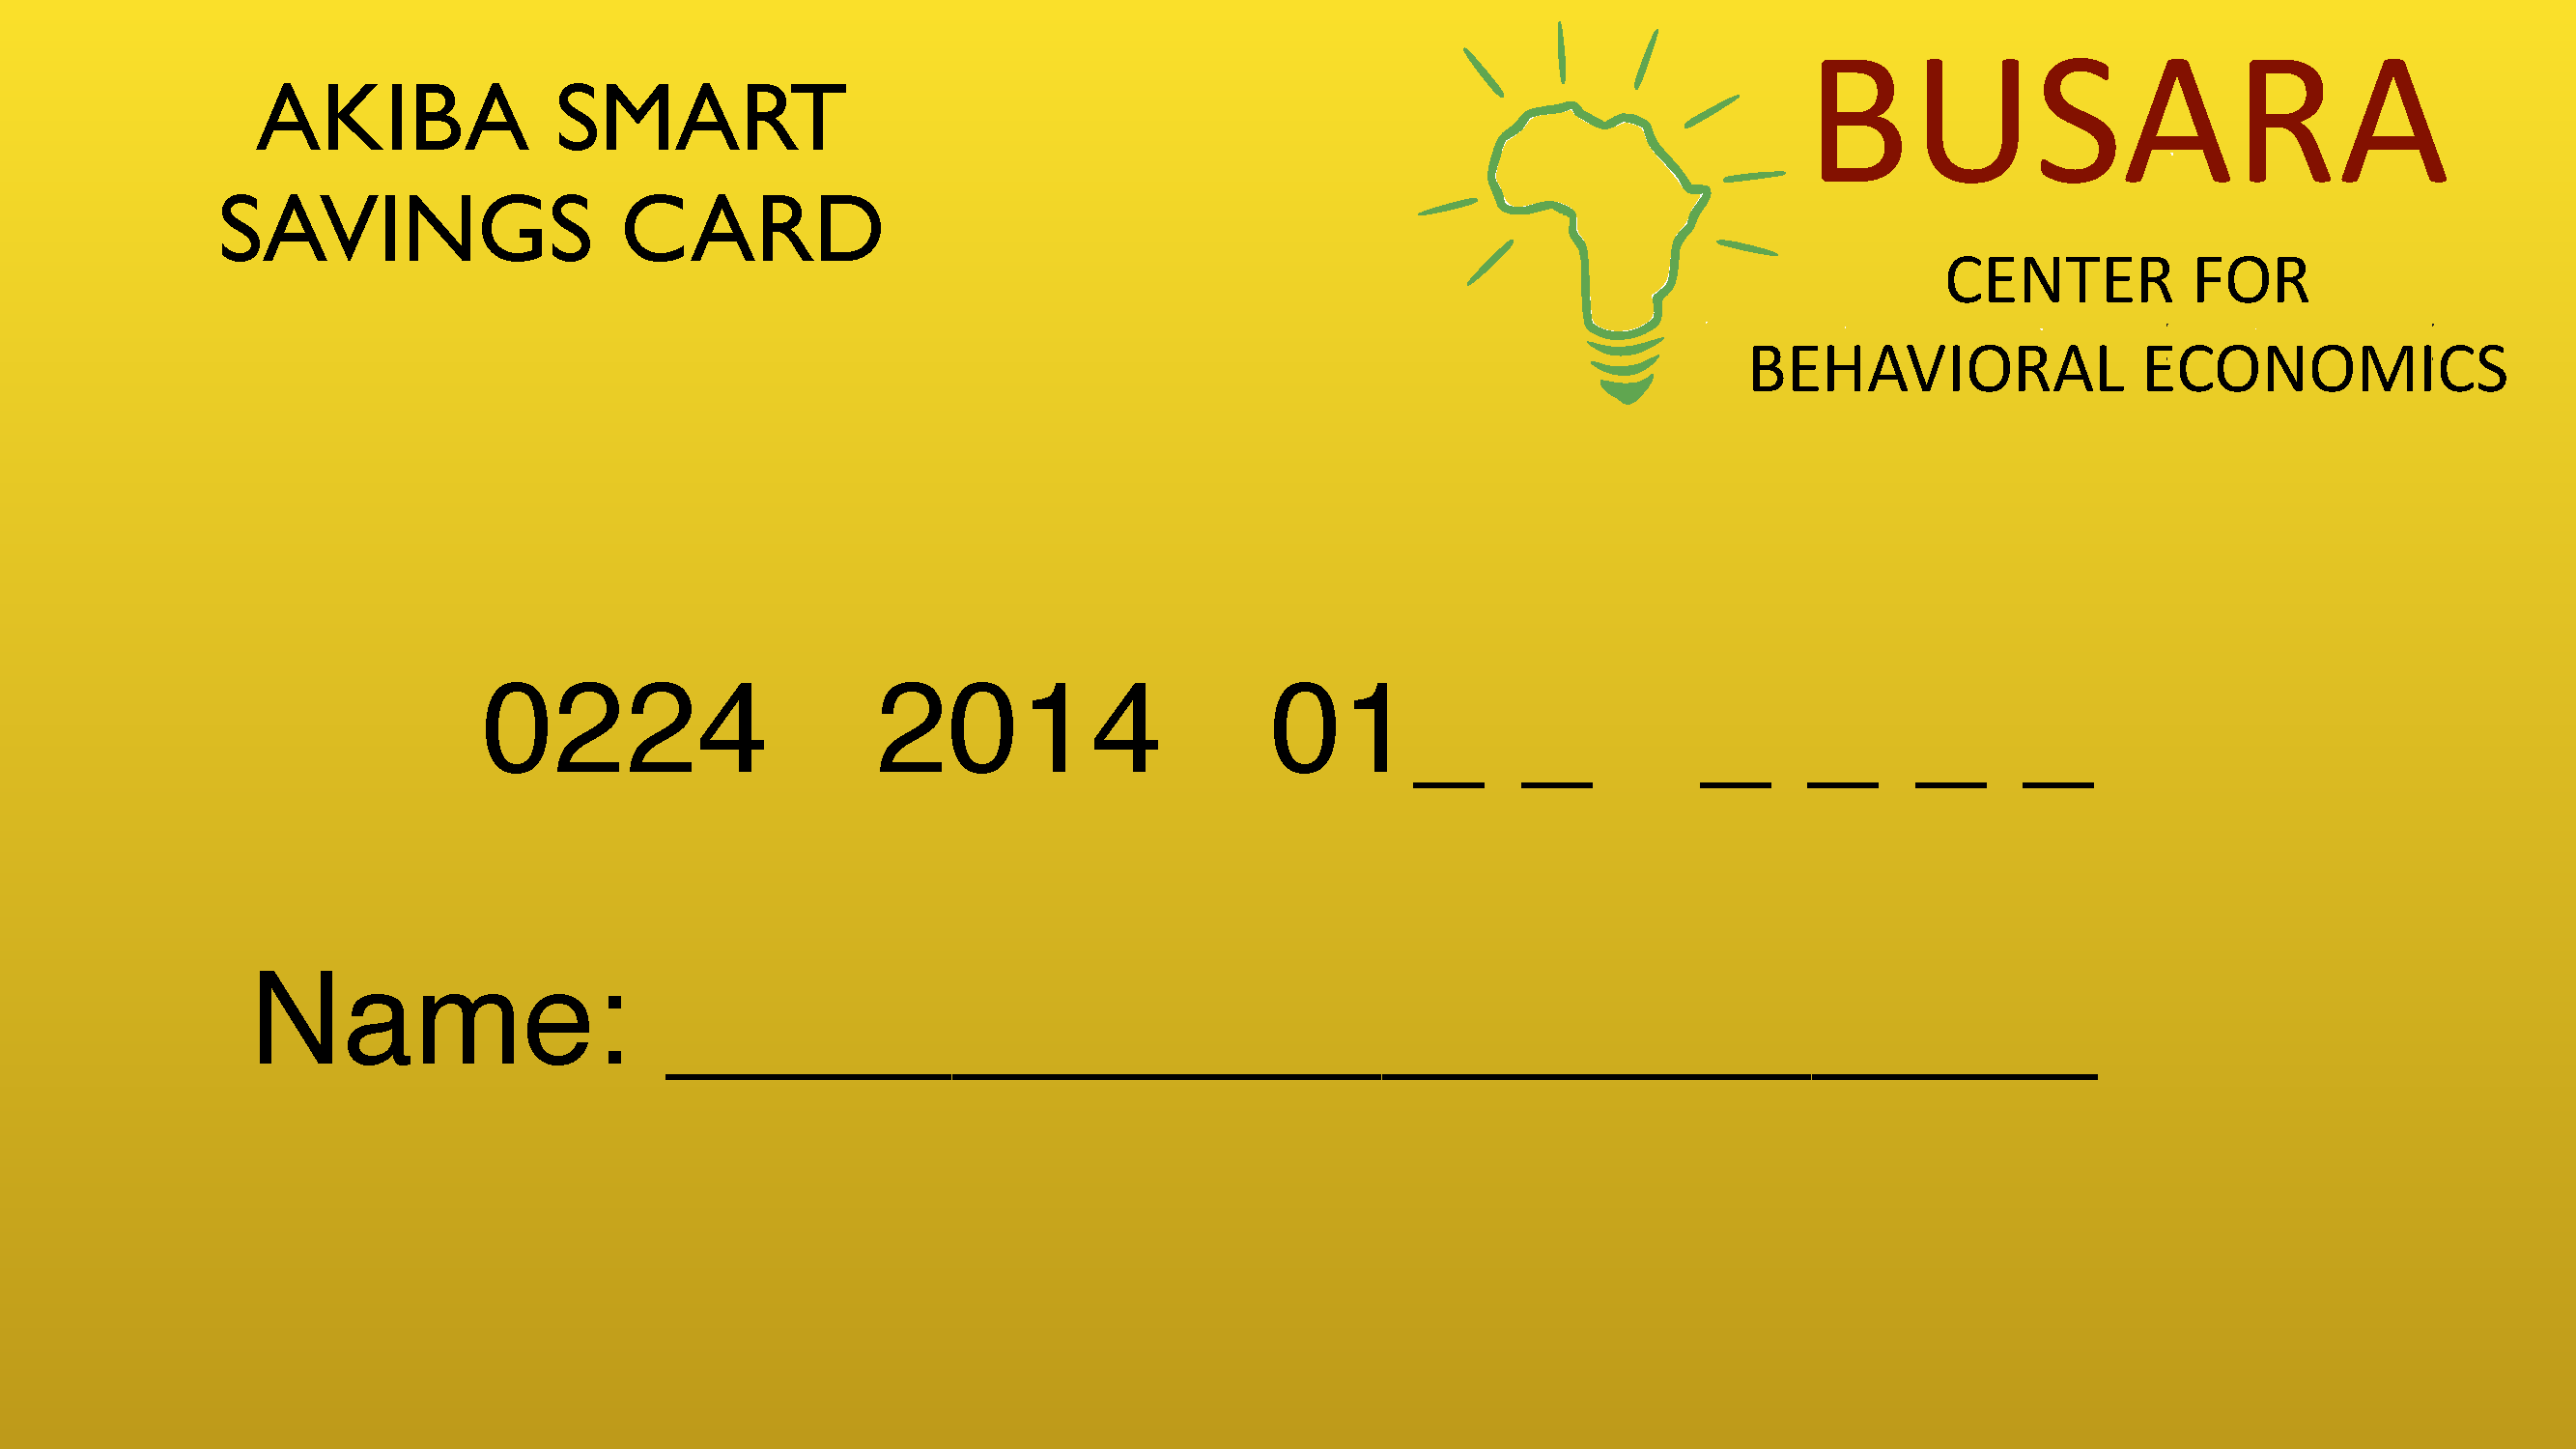
\includegraphics[width=0.45\textwidth]{../../figures/id_front_control.pdf} & 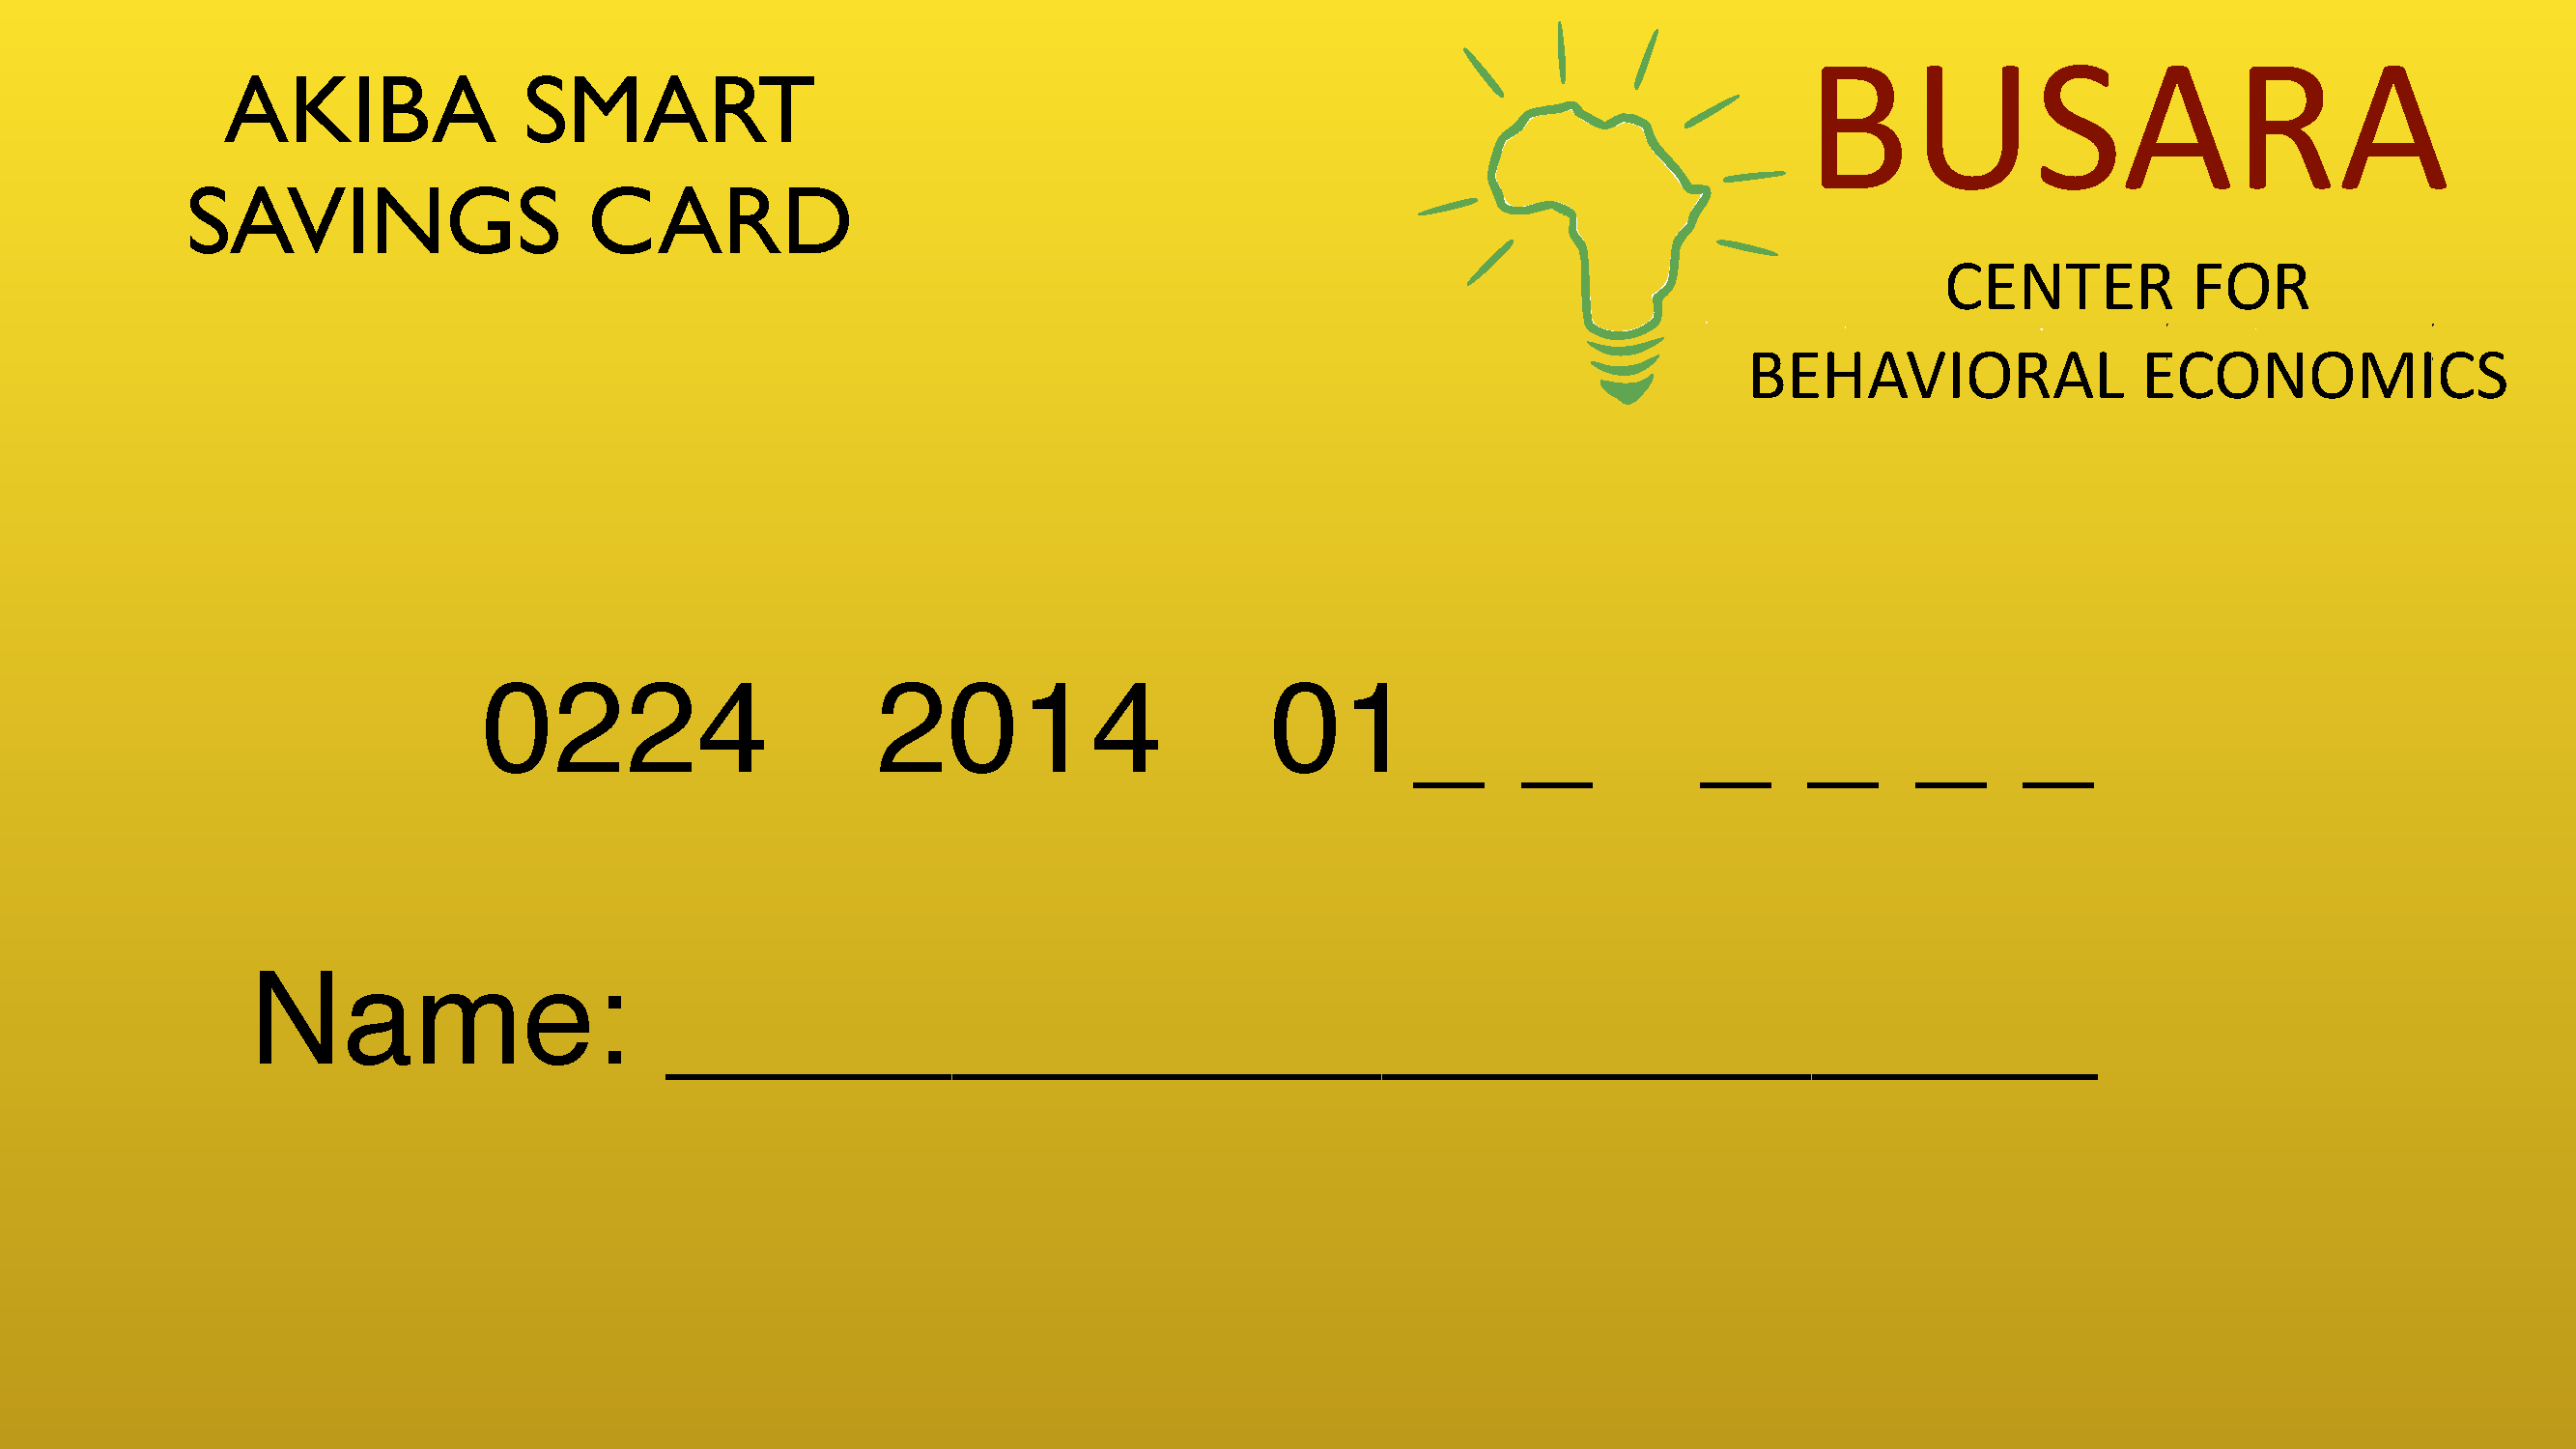
\includegraphics[width=0.45\textwidth]{../../figures/id_front_lottery.pdf} \\
        (a) Front & (b) Front \\
        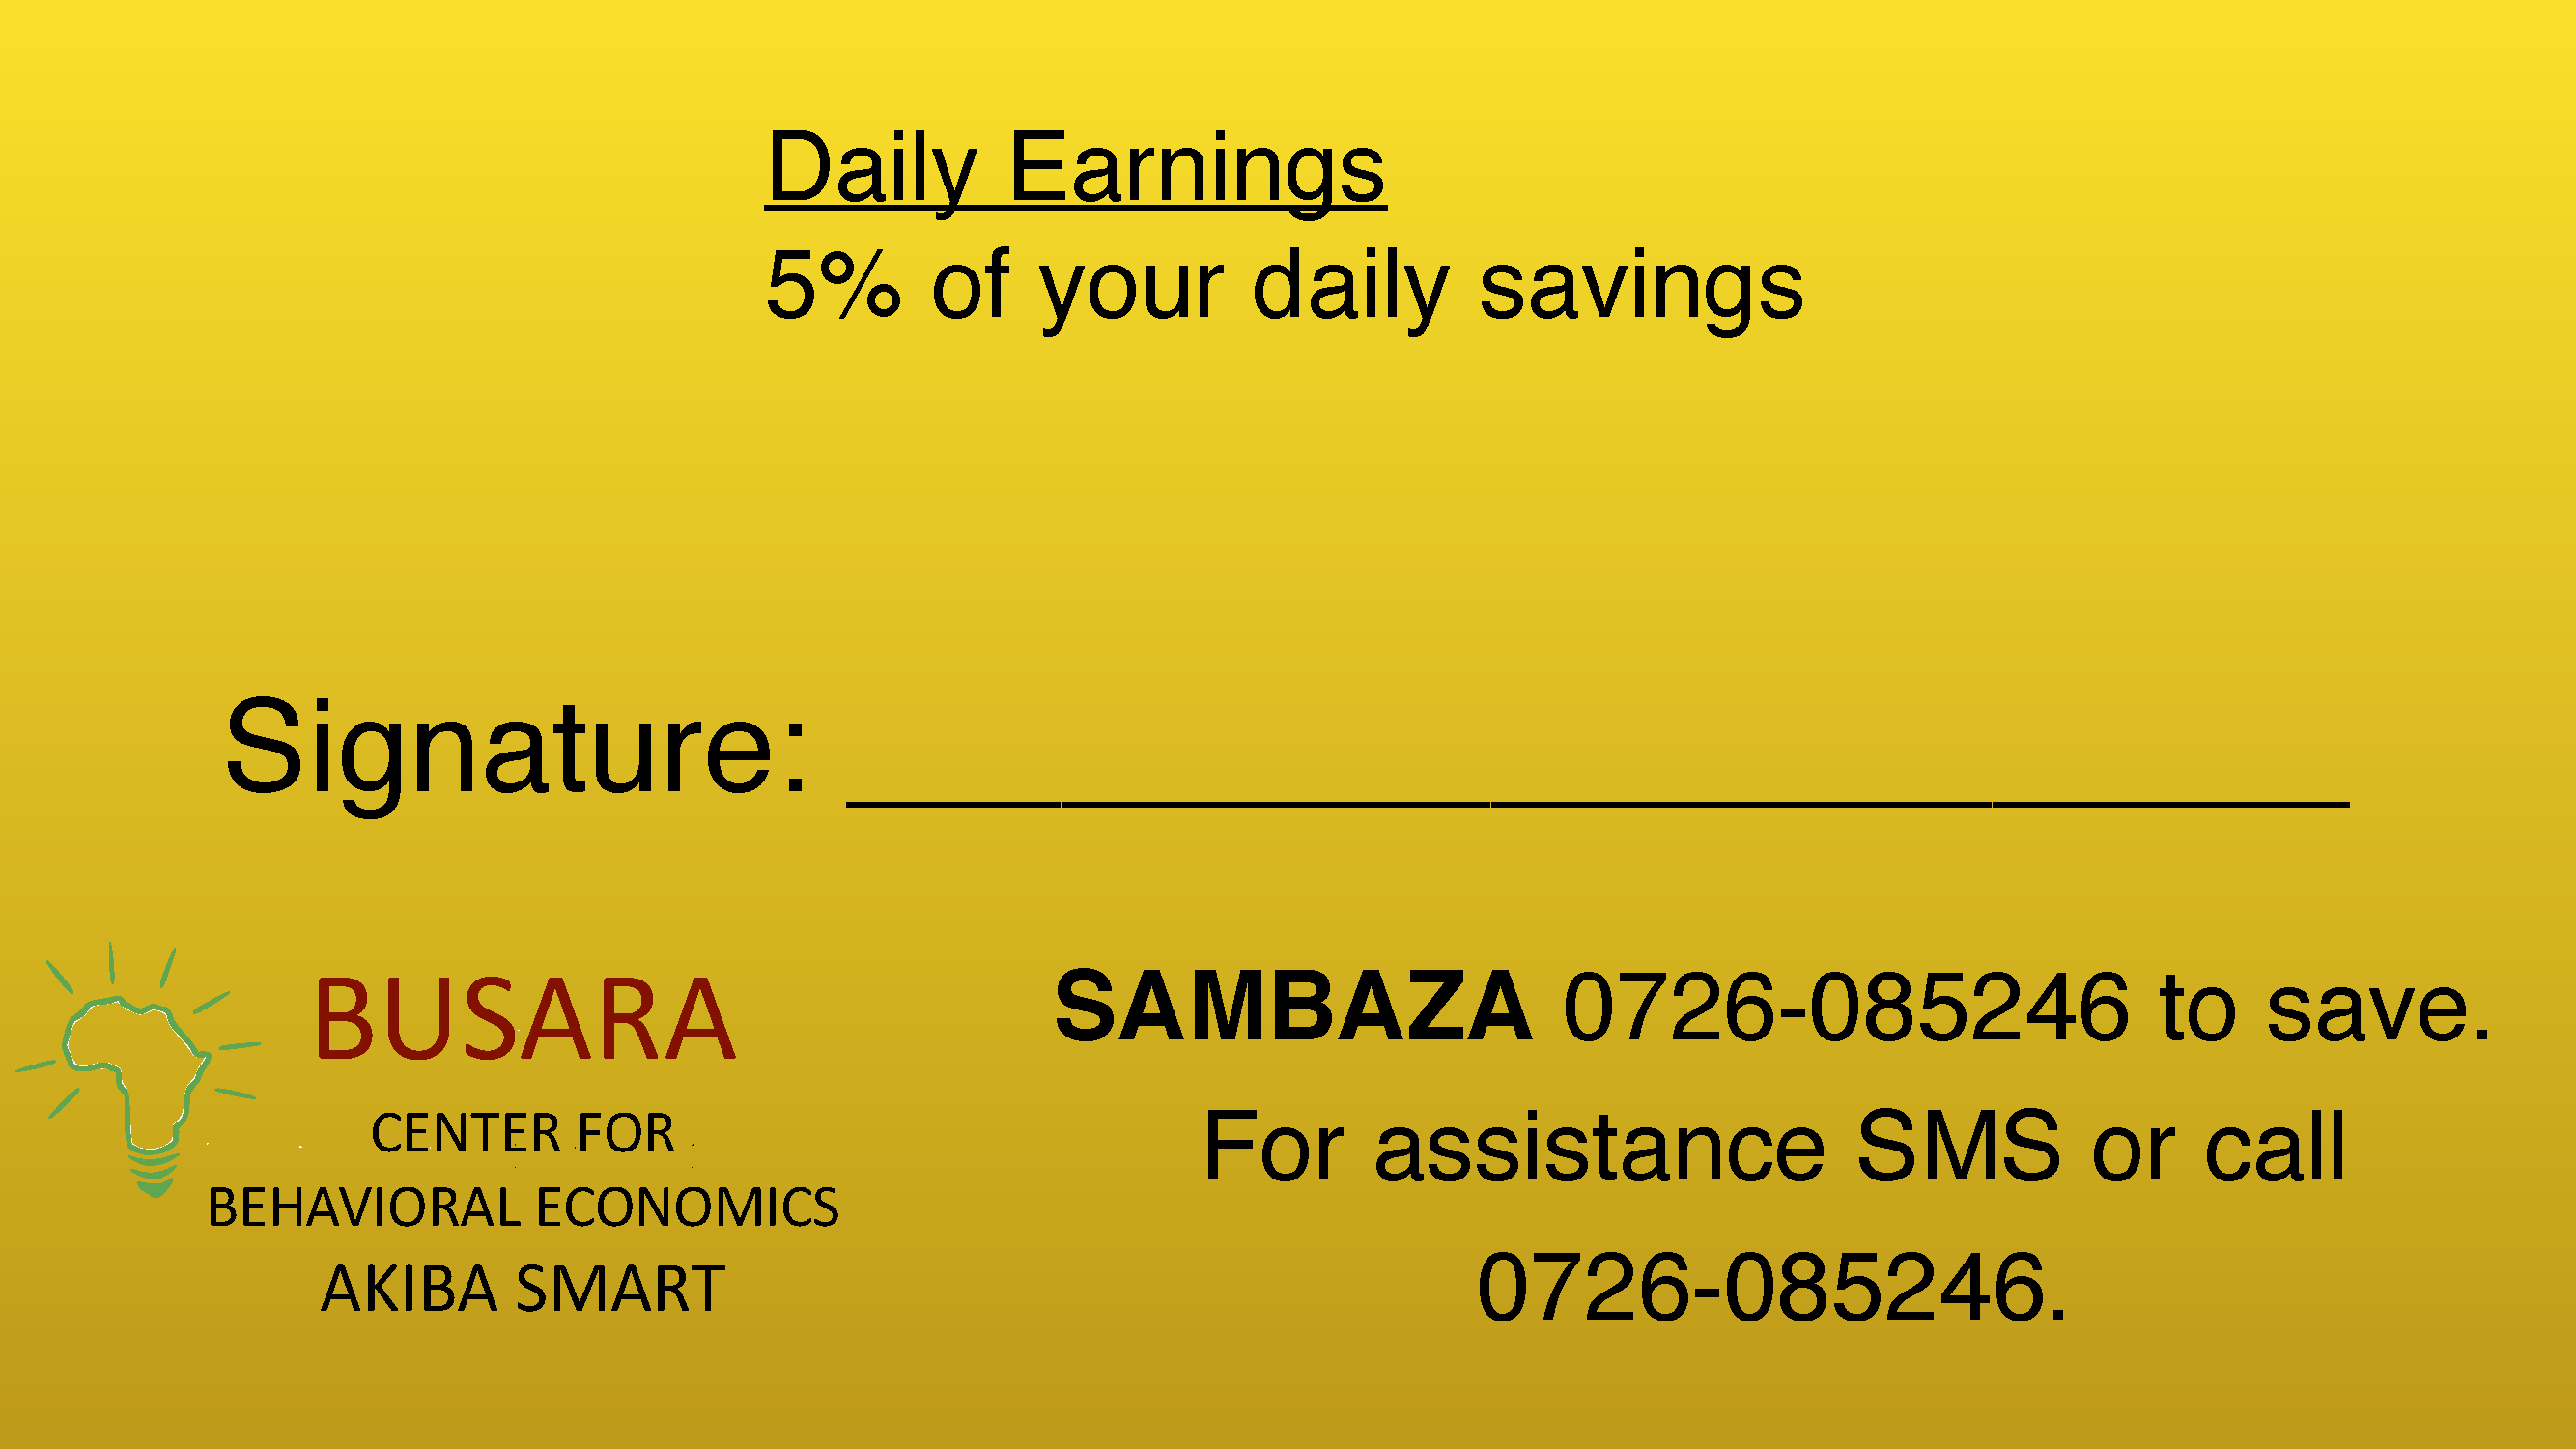
\includegraphics[width=0.45\textwidth]{../../figures/id_back_control.pdf} & 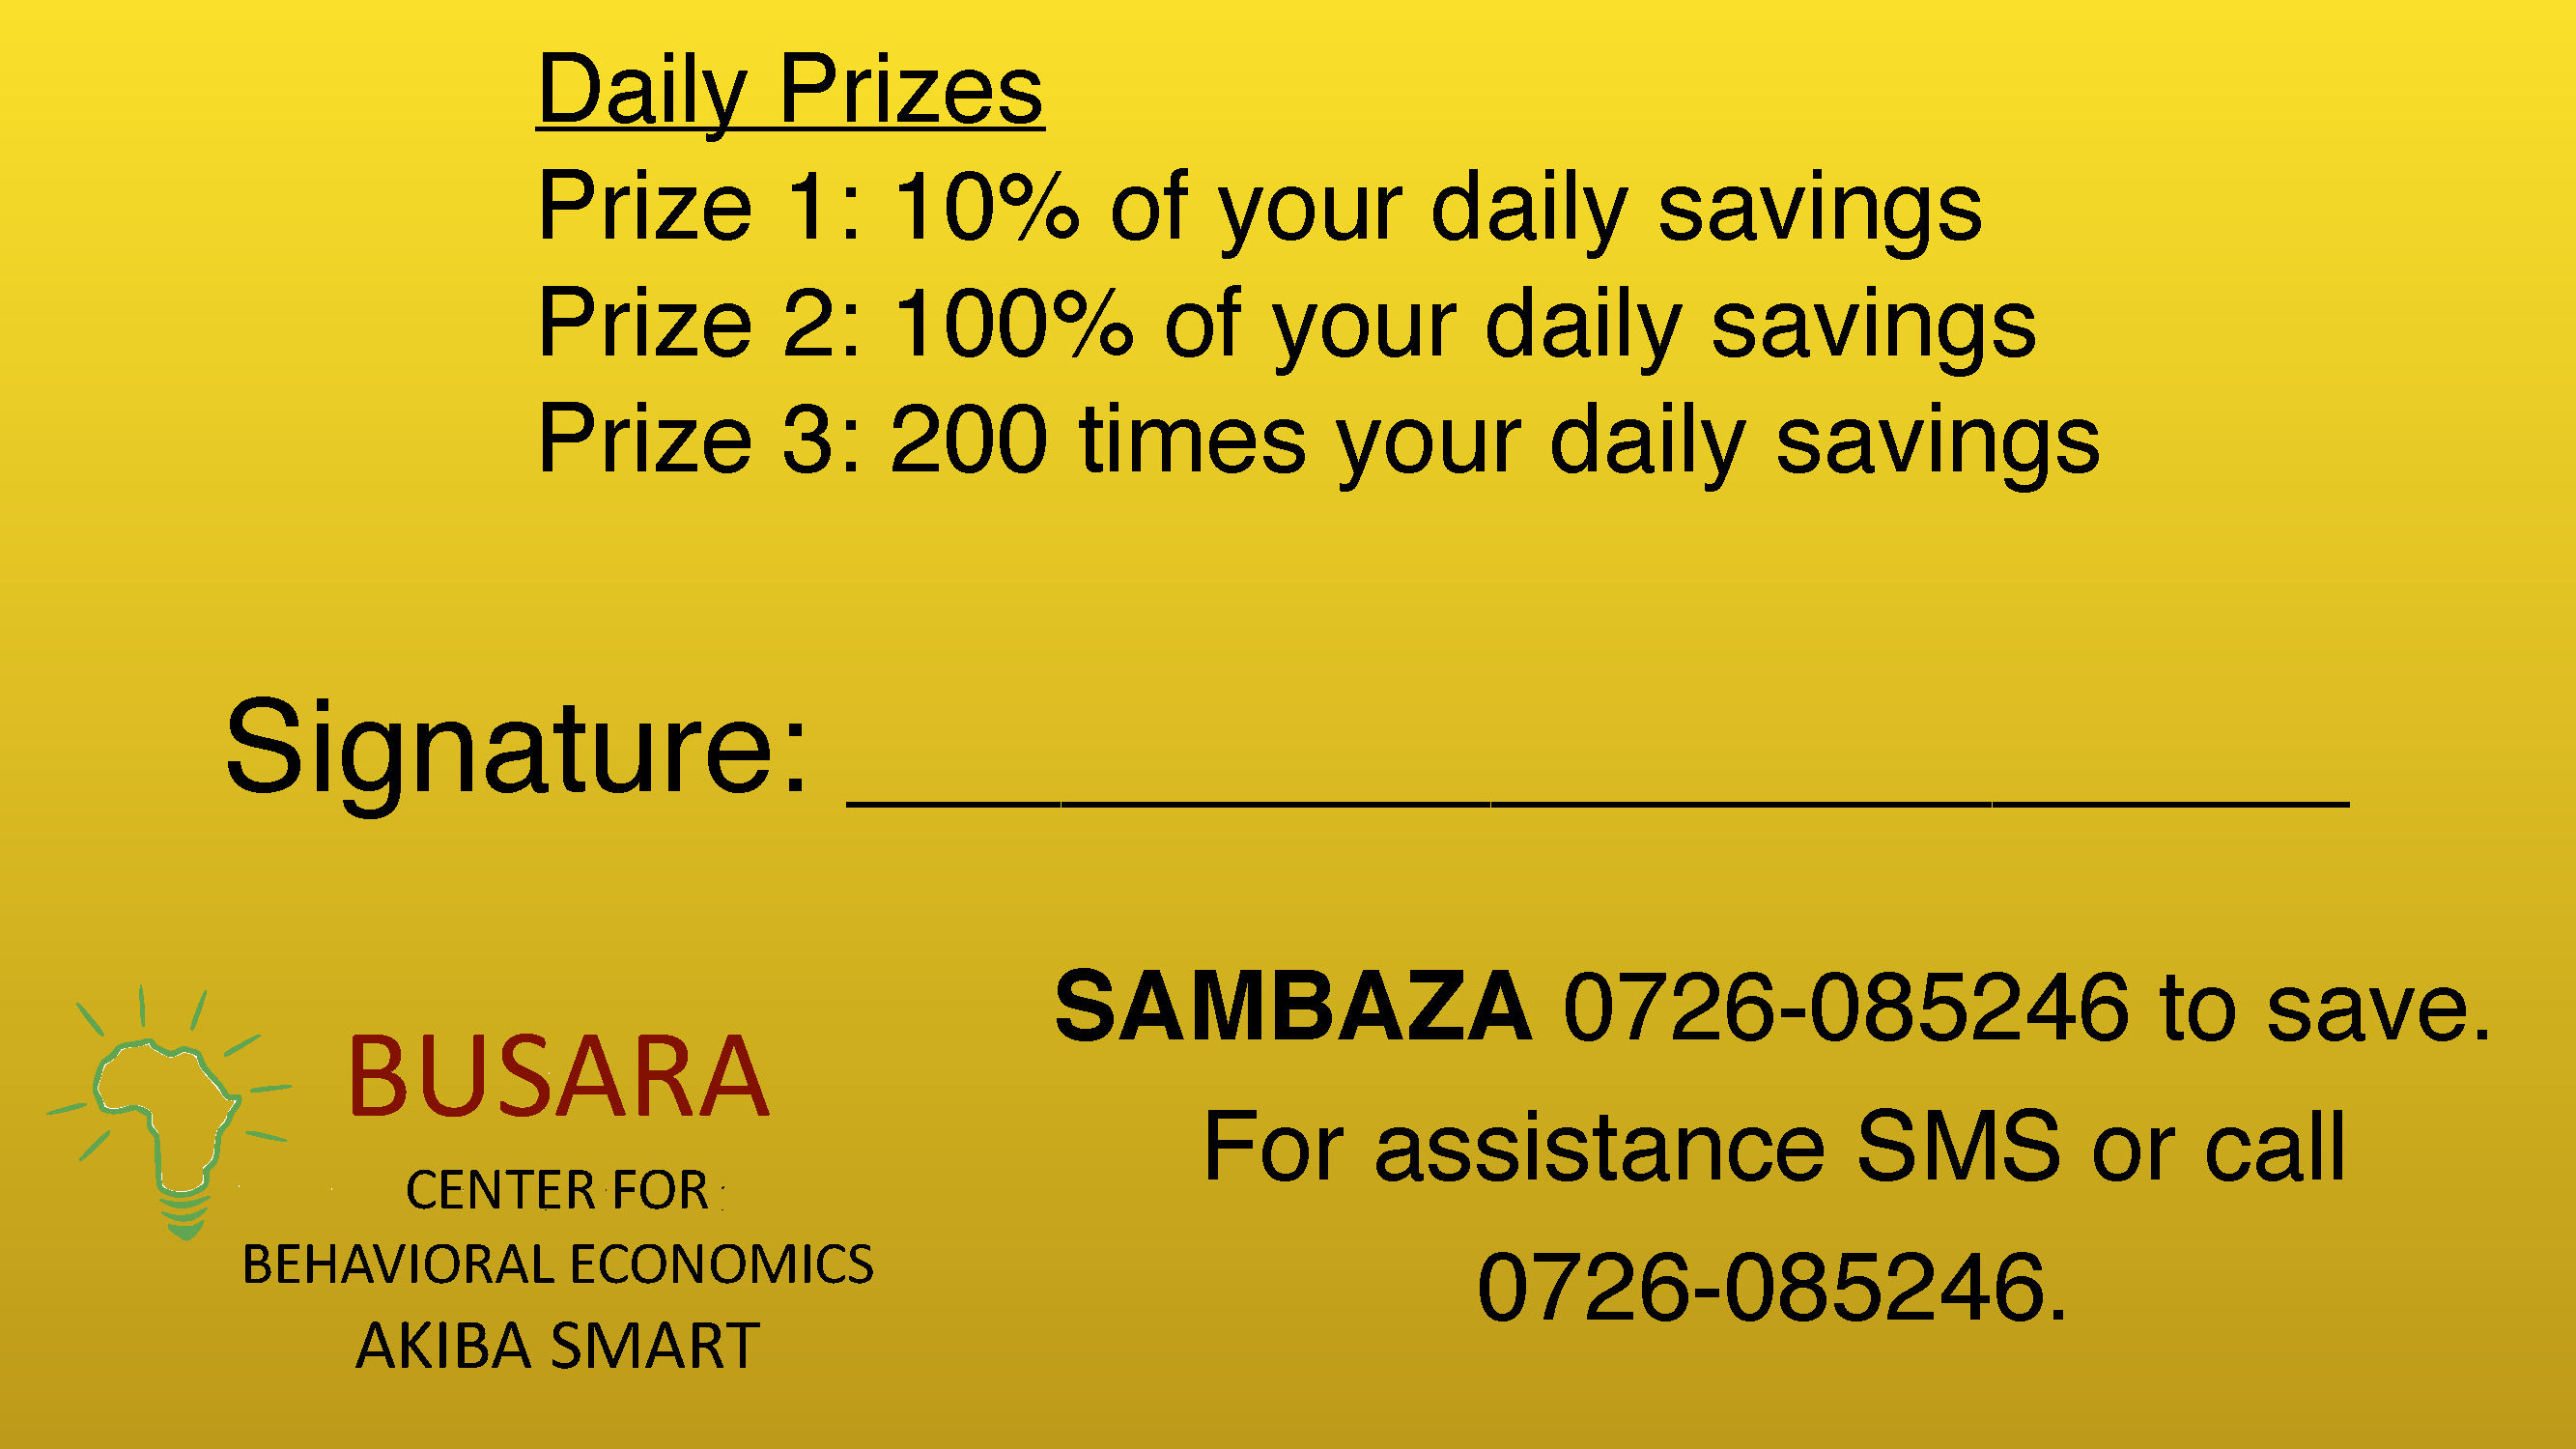
\includegraphics[width=0.45\textwidth]{../../figures/id_back_lottery.pdf} \\
        (c) Back (Control) & (d) Back (Lottery) \\
        \end{tabular}
        \end{figure}

        \clearpage

        \subsubsection{SMS reminders (Control)}

            \begin{itemize}
                \item \underline{Reminder}: ``{Name}, remember to save XX or more today to earn 5\% daily interest. Sambaza *140*XX*Phone to save''
                \item \underline{Upon receipt of airtime}: ``You saved XX. You earned 5\% interest!  QQ was deposited into your account. Your balance is ZZ.''
            \end{itemize}

        \subsubsection{SMS reminders (Lottery)}

            \begin{itemize}
                \item \underline{Reminder}: ``{Name}, remember to buy your ticket today (this week) by saving XX. Sambaza *140*XX*Phone to save''
                \item \underline{Upon receipt of airtime}: ``You saved XX. You purchased your ticket. Your lucky numbers are AA-BB. Your balance is ZZ.''
            \end{itemize}

        \subsubsection{SMS reminders (Regret)}

            \begin{itemize}
                \item \underline{Reminder}: ``{Name}, your lucky numbers today (this week) are AA-BB. Keep them by saving XX. Sambaza *140*XX*Phone to save''
                \item \underline{Upon receipt of airtime}: ``You saved XX. You purchased your ticket. Your lucky numbers are AA-BB. Your balance is ZZ.''
            \end{itemize}

        \subsubsection{Lottery administration (for treatment groups)}

            \begin{itemize}
                \item \underline{Winning numbers}: ``Yesterday's (last week's) lucky numbers were CC-DD. Winners receive PPP Ksh. Save today (this week) to play again!''
                \item \underline{Winners}: ``Your lucky numbers were AA-BB. Congratulations!  You won PPP Ksh!  Win again today (this week) by saving.''
                \item \underline{Losers}: ``Your lucky numbers were AA-BB. You did not win. Try again today (this week) by saving.''
                \item \underline{Losers in regret group}: ``Your lucky numbers were AA-BB. You would have won, but you did not save enough to buy your ticket!  Don't miss you again, save to play.''
            \end{itemize}

        \subsubsection{Other}

            \begin{itemize}
                \item \underline{Upon receipt of an incoming SMS}: ``Your balance is ZZ. Save YY to buy your ticket (reach your match) OR You have reached your goal today (this week). Save more, Sambaza *140*XX*Phone.''
                \item \underline{Upon receipt of airtime from unknown number}: ``This number is not known in the system. What is your standard phone number (10-digits)?''
                \item \underline{If reply is not understood (return airtime via Sambaza)}: ``This is not a valid response. We are returning your airtime. Please save using your phone only. Call Phone for help.''
            \end{itemize}

    \subsection{Laboratory instructions}

        \subsubsection{Coin toss task}

            For the next task your payoff will depend on a coin flip.  You will win money if it is a heads or if it is a tails.  You must decide which payoffs for heads and tails you prefer. The exact amount of money you will win will depend on which side the coin landed on. On the next screen you will see 6 different values for heads and tails. You make a SINGLE decision on which coin you prefer and remember that you can only flip one of the coins and only once. There are no right or wrong answers, only your preference.

        \subsubsection{Titration task}

            On the following screen you will find a series of questions. In each question, you are asked to choose between Option A and Option B. If you choose Option A, you will get a smaller amount but sooner. If you choose Option B, you will get a larger amount but later. Please choose the option you prefer. There are no right or wrong answers. After you make all your choices, the computer will randomly pick one of the questions and your payment will be determined by the option you chose in that question. Remember that the computer will pick only one question and any question could be picked. Therefore it is in your interest to answer each question as if it is the only question you are answering.

        \subsubsection{Lottery task}

            In this game, FIRST the computer will randomly chose 4 numbers, each between 0 and 9, to create a lottery ticket for you. For example, your lottery ticket could be: 5067 Then the computer will randomly choose 4 numbers again, each between 0 and 9, to create the winning lottery ticket. For example the winning ticket could be 5645 The lottery prizes are as follows:

            PRIZE 1 (5KSH): If the FIRST OR SECOND number of your lottery ticket match the first OR second number of the winning ticket, your ticket will win prize 1.

            PRIZE 2 (50KSH): If the FIRST AND SECOND number of your lottery ticket match the first AND second number of the winning ticket in the same order, your ticket will win prize 2.

            PRIZE 3 (5000KSH): If ALL NUMBERS of your ticket match all numbers of the winning ticket in the same order, your ticket will win prize 3.

        \subsubsection{Canadian Problem Gambling Index}

        In the last 12 months how often have you [or have for item 7]? 0 = Never, 1 = Sometimes, 2 = Most of the time, 3 = Almost always

        \begin{enumerate}
            \item Bet more than you could really afford to lose?
        	\item Needed to gamble with larger amounts of money to get the same feeling of excitement?
        	\item Gone back another day to try and win back the money you lost?
        	\item Borrowed money or sold anything to get money to gamble?
        	\item Felt that you might have a problem with gambling?
        	\item Felt that gambling has caused you health problems, including stress and anxiety?
        	\item People criticized your betting or told you that you have a gambling problem, whether or not you thought it was true?
        	\item Felt your gambling has caused financial problems for you or your household?
        \end{enumerate}

        In the past month, how often have you done the following? 0 = Never, 1 = 1-4 times, 2 = Daily, 3 = multiple times per day

        \begin{enumerate}
        	\item Bet money on a sporting event
        	\item Played the lottery (Charity Sweepstakes)
        	\item Played cards or another game for money (billards, checkers, etc)
        	\item In the past month, how often have you gambled in all activities?
        	\item Participated in an SMS promotion (Safaricom ''Bonyeza Ushinde'' ''Tetemesha'' or other)
        \end{enumerate}

	\clearpage

% \section{Description of variables}
%
% 	We estimate treatment effects on measured savings behavior. The main outcome variables we are interested in are:
%
% 		\begin{enumerate}
% 		\item Average savings over the entire study period.
% 		\item Average savings over the first and second 30-day period.
% 		\item Average number of active days and average number of transactions.
% 		\item Average length of the streaks, i.e. the highest number of consecutive days with a positive daily balance for each person.
% 		\end{enumerate}
%
% 	Aside from the overall savings behavior, we additionally estimate the effect of the program on:
%
% 		\begin{enumerate}
% 		\item Amount withdrawn mid-project
% 		\item Monthly savings
% 		\item Whether subject saves
% 		\item Monthly M-Pesa savings
% 		\item Whether subject saves with a ROSCA
% 		\item Temptation to gamble
% 		\item Gambling behavior
% 		\item How often subject discussed savings program with family and friends
% 		\item Trust in the savings program
% 		\item Satisfaction with saving behavior in the program
% 		\item Continuation with the savings program
% 		\item Self-perception as a saver
% 		\item Trust in the savings program
% 		\end{enumerate}

\section{Summary Statistics}

	\subsection{Balance checks}

        \begin{table}[h]\centering \def\sym#1{\ifmmode^{#1}\else\(^{#1}\)\fi} \caption{Baseline balance by treatment group} \label{tab:sum-ysumall} \maxsizebox*{\textwidth}{\textheight}{ \begin{threeparttable} \begin{tabular}{l*{5}{c}} \toprule
          &\multicolumn{1}{c}{(1)}&\multicolumn{1}{c}{(2)}&\multicolumn{1}{c}{(3)}&\multicolumn{1}{c}{(4)}&\multicolumn{1}{c}{(5)}\\
          &\multicolumn{1}{c}{\specialcell{No Feedback -\\Control}}&\multicolumn{1}{c}{\specialcell{PLS -\\Control}}&\multicolumn{1}{c}{\specialcell{No Feedback -\\PLS}}&\multicolumn{1}{c}{\specialcell{Control mean\\(SD)}}&\multicolumn{1}{c}{Obs.}\\
\midrule
Female    &     0.07&     0.10&     0.03&     0.52&      311\\
          &   (0.07)&   (0.07)&   (0.07)&   (0.50)&         \\
Age       &     0.78&     0.72&    -0.05&    30.75&      311\\
          &   (1.39)&   (1.34)&   (1.35)&   (9.83)&         \\
Completed std. 8&    -0.02&    -0.02&     0.00&     0.99&      311\\
          &   (0.02)&   (0.02)&   (0.02)&   (0.10)&         \\
Married/co-habitating&     0.10&     0.09&    -0.01&     0.42&      311\\
          &   (0.07)&   (0.07)&   (0.07)&   (0.50)&         \\
No. of children&     0.23&     0.24&     0.01&     1.75&      311\\
          &   (0.24)&   (0.25)&   (0.25)&   (1.70)&         \\
Currently saves&     0.05&    -0.10&    -0.15&     0.56&      311\\
          &   (0.07)&   (0.07)&   (0.07)&   (0.50)&         \\
Total savings last month&   -17.81&    -7.04&    10.77&    58.82&      311\\
          &  (11.88)&  (12.55)&   (9.23)& (106.26)&         \\
Monthly income&    -3.68&    -0.59&     3.09&   112.05&      311\\
          &  (17.63)&  (16.85)&  (15.46)& (137.13)&         \\
Employment status&     0.05&    -0.03&    -0.08&     0.50&      311\\
          &   (0.07)&   (0.07)&   (0.07)&   (0.50)&         \\
Coefficient of relative risk aversion&     0.08&    -0.03&    -0.12&     1.16&      311\\
          &   (0.18)&   (0.17)&   (0.18)&   (1.27)&         \\
Locus of control&     0.48&    -0.83&    -1.31&    69.81&      311\\
          &   (1.40)&   (1.46)&   (1.37)&  (10.78)&         \\
Standardized CPGI&    -0.11&    -0.22&    -0.11&    -0.00&      311\\
          &   (0.13)&   (0.12)&   (0.12)&   (1.00)&         \\
Exp. discount factor&    -0.05&    -0.01&     0.04&     0.33&      311\\
          &   (0.03)&   (0.03)&   (0.03)&   (0.20)&         \\
\midrule Joint test \emph{p}-value&     0.44&     0.72&     0.42&         &         \\
\bottomrule \end{tabular} \begin{tablenotes}[flushleft] \footnotesize \item \emph{Notes:} The first three columns report the difference of means across treatment groups with standard errors in parentheses. Column 4 reports the mean of the control group with SD in parentheses. The bottom row reports the \(p\)-value of a joint test of significance for each hypothesis. \end{tablenotes} \end{threeparttable} } \end{table}

% File produced by sum-treat.do with /Users/justin/Repos/akiba-lottery-pub/data/clean/akiba_wide.dta on 15:49:29 12 Aug 2020 by user justin on Stata 13.1 with seed X53d8cd0fc43f462544a474abacbdd93d00044a8f
        \begin{table}[h]\centering \def\sym#1{\ifmmode^{#1}\else\(^{#1}\)\fi} \caption{Baseline balance by treatment group for endline sample} \label{tab:sum-eltreatall} \maxsizebox*{\textwidth}{\textheight}{ \begin{threeparttable} \begin{tabular}{l*{5}{c}} \toprule
          &\multicolumn{1}{c}{(1)}&\multicolumn{1}{c}{(2)}&\multicolumn{1}{c}{(3)}&\multicolumn{1}{c}{(4)}&\multicolumn{1}{c}{(5)}\\
          &\multicolumn{1}{c}{\specialcell{Lottery -\\Control}}&\multicolumn{1}{c}{\specialcell{Regret -\\Control}}&\multicolumn{1}{c}{\specialcell{Lottery -\\Regret}}&\multicolumn{1}{c}{\specialcell{Control mean\\(SD)}}&\multicolumn{1}{c}{Obs.}\\
\midrule
Female    &     0.05&     0.09&     0.04&     0.53&      284\\
          &   (0.07)&   (0.07)&   (0.07)&   (0.50)&         \\
Age       &    -0.18&     0.24&     0.42&    31.37&      284\\
          &   (1.48)&   (1.43)&   (1.42)&  (10.11)&         \\
Completed std. 8&    -0.02&     0.00&     0.02&     0.99&      284\\
          &   (0.02)&   (0.01)&   (0.02)&   (0.10)&         \\
Married/co-habitating&     0.08&     0.07&    -0.01&     0.44&      284\\
          &   (0.07)&   (0.07)&   (0.07)&   (0.50)&         \\
No. of children&    -0.01&     0.10&     0.11&     1.88&      284\\
          &   (0.25)&   (0.26)&   (0.25)&   (1.73)&         \\
Currently saves&     0.05&    -0.05&    -0.09&     0.54&      284\\
          &   (0.07)&   (0.07)&   (0.07)&   (0.50)&         \\
Total savings last month&   -18.63&    -4.82&    13.81&    58.75&      284\\
          &  (12.01)&  (12.88)&   (9.78)& (100.77)&         \\
Monthly income&    -9.42&    -5.24&     4.18&   117.77&      284\\
          &  (18.93)&  (17.87)&  (16.18)& (140.31)&         \\
Employment status&     0.05&    -0.05&    -0.09&     0.51&      284\\
          &   (0.07)&   (0.07)&   (0.07)&   (0.50)&         \\
Coefficient of relative risk aversion&     0.16&    -0.01&    -0.17&     1.13&      284\\
          &   (0.19)&   (0.18)&   (0.19)&   (1.25)&         \\
Locus of control&     0.69&    -0.95&    -1.63&    69.79&      284\\
          &   (1.50)&   (1.56)&   (1.45)&  (11.05)&         \\
Standardized CPGI&    -0.12&    -0.20&    -0.09&    -0.02&      284\\
          &   (0.13)&   (0.13)&   (0.12)&   (0.97)&         \\
Exp. discount factor&-0.06\sym{**}&    -0.02&     0.04&     0.33&      284\\
          &   (0.03)&   (0.03)&   (0.03)&   (0.20)&         \\
\midrule Joint test \emph{p}-value&     0.52&     0.94&     0.64&         &         \\
\bottomrule \end{tabular} \begin{tablenotes}[flushleft] \footnotesize \item \emph{Notes:} These results are restricted to the sample of participants who completed the endline survey. The first three columns report the difference of means across treatment groups with SEs in parentheses. Column 4 reports the mean of the control group with SD in parentheses. The bottom row reports the \(p\)-value of a joint test of significance for each hypothesis. * denotes significance at 10 pct., ** at 5 pct., and *** at 1 pct. level. \end{tablenotes} \end{threeparttable} } \end{table}

% File produced by sum-eltreat.do with /Users/justin/Repos/akiba-lottery-pub/data/clean/akiba_wide.dta on 10:03:59 14 Jun 2019 by user justin on Stata 13.1 with seed X53d8cd0fc43f462544a474abacbdd93d00044a8f
        \begin{table}[h]\centering \def\sym#1{\ifmmode^{#1}\else\(^{#1}\)\fi} \caption{Self-selection by treatment group} \label{tab:tab-select} \maxsizebox*{\textwidth}{\textheight}{ \begin{threeparttable} \begin{tabular}{l*{4}{c}} \toprule
                &\multicolumn{4}{c}{Self-selection into treatment groups}                   \\\cmidrule(lr){2-5}
                & Interest         &  Lottery         &   Regret         &    Total         \\
\midrule
Interest        &       39         &       52         &        3         &       94         \\
Lottery         &       27         &       54         &       14         &       95         \\
Regret          &       32         &       42         &       21         &       95         \\
Total           &       98         &      148         &       38         &      284         \\
\bottomrule \end{tabular} \begin{tablenotes}[flushleft] \footnotesize \item \emph{Notes:} This table reports the number of participants self-selecting into the treatment conditions after completing the study, disaggregated by original treatment assignment. \end{tablenotes} \end{threeparttable} } \end{table}

% File produced by akiba_summary.do with /n/homeserver2/user2a/justinra/repos/akiba-lottery-pub/data/clean/akiba_wide.dta on 02:46:18 15 Feb 2018 by user justinra on Stata 13.1 with seed X53d8cd0fc43f462544a474abacbdd93d00044a8f

        \begin{table}[htbp]\centering \def\sym#1{\ifmmode^{#1}\else\(^{#1}\)\fi} \caption{Expected and observed lottery results} \label{tab:tab-lottery} \maxsizebox*{\paperwidth}{\paperheight}{ \begin{threeparttable} \begin{tabular}{l*{3}{c}} \toprule
                    &        Freq.&         Pct. observed&      Pct. expected\\
\midrule
No match                   &        7065&       81.49&       62.43\\
One match                   &        1518&       17.51&       22.22\\
Two matches                   &          86&        0.99&       1.23\\
Complete match                   &           1&        0.01&      0.00\\
\bottomrule \end{tabular} \begin{tablenotes}[flushleft] \footnotesize \item \emph{Notes:} The first column tabulates the frequency of observed lottery ticket matches. The second and third columns report the observed and expected probabilities, respectively, of each type of lottery match. A lottery ticket was a random sequence of four numbers between 1 and 9, inclusive. Prizes were awarded according to how well a participant's lottery numbers matched the winning numbers. If the first or second numbers matched, a 10\% match of savings was awarded. If \emph{both} the first and second numbers matched, a 100\% match of savings was awarded. Finally if all numbers matched, a prize of 200 times the daily savings was awarded. \end{tablenotes} \end{threeparttable} } \end{table}


	\clearpage

    \subsection{Sample attrition}

        \begin{table}[htbp]\centering \def\sym#1{\ifmmode^{#1}\else\(^{#1}\)\fi} \caption{Treatment group by participation at endline} \label{tab:tab-balance} \maxsizebox*{\textwidth}{\textheight}{ \begin{threeparttable} \begin{tabular}{l*{3}{c}} \toprule
                &\multicolumn{3}{c}{Participation at endline}            \\\cmidrule(lr){2-4}
                & Attrited         &Completed         &    Total         \\
\midrule
Interest        &       11         &       94         &      105         \\
Lottery         &        8         &       95         &      103         \\
Regret          &        8         &       95         &      103         \\
Total           &       27         &      284         &      311         \\
\bottomrule \end{tabular} \begin{tablenotes}[flushleft] \footnotesize \item \emph{Notes:} This table reports the number of observations in the endline survey by treatment group. Columns 1 and 2 reports the number of participants who completed the baseline survey but not endline and those who completed both surveys, repsectively. \end{tablenotes} \end{threeparttable} } \end{table}

% File produced by akiba_summary.do with /Users/Justin/Repos/akiba-lottery-pub/data/clean/akiba_wide.dta on 15:12:37 18 May 2017 by user Justin on Stata 13.1 with seed X53d8cd0fc43f462544a474abacbdd93d00044a8f

        \begin{table}[htbp]\centering \def\sym#1{\ifmmode^{#1}\else\(^{#1}\)\fi} \caption{Attrition by treatment group} \label{tab:reg-attr} \maxsizebox*{\paperwidth}{\paperheight}{ \begin{threeparttable} \begin{tabular}{l*{1}{c}} \toprule
                &\multicolumn{1}{c}{Unobserved at endline}\\
\midrule
Lottery         &    -0.03         \\
                &   (0.04)         \\
Regret          &    -0.03         \\
                &   (0.04)         \\
Constant        &     0.10\sym{***}\\
                &   (0.03)         \\
\midrule
Observations    &      311         \\
Adjusted \(R^{2}\)&   -0.004         \\
Difference p-value&     1.00         \\
Joint p-value   &     0.75         \\
\bottomrule \end{tabular} \begin{tablenotes}[flushleft] \footnotesize \item \emph{Notes:} This table reports a regression of selection on each of the treatment arms. Standard errors are in parentheses. * denotes significance at 10 pct., ** at 5 pct., and *** at 1 pct. level. \end{tablenotes} \end{threeparttable} } \end{table}

% File produced by akiba-estimate.do with /Users/Justin/Repos/akiba-lottery-pub/data/clean/akiba_wide.dta on 17:14:52 25 Mar 2017 by user Justin on Stata 13.1 with seed X53d8cd0fc43f462544a474abacbdd93d00044a8f
        \begin{table}[h]\centering \def\sym#1{\ifmmode^{#1}\else\(^{#1}\)\fi} \caption{Baseline balance by attrition status} \label{tab:sum-attrall} \maxsizebox*{\textwidth}{\textheight}{ \begin{threeparttable} \begin{tabular}{l*{3}{c}} \toprule
          &\multicolumn{1}{c}{(1)}&\multicolumn{1}{c}{(2)}&\multicolumn{1}{c}{(3)}\\
          &\multicolumn{1}{c}{\specialcell{Completed -\\attrited}}&\multicolumn{1}{c}{\specialcell{Mean (SD)\\of completed}}&\multicolumn{1}{c}{Obs.}\\
\midrule
Female    &    -0.02&     0.58&      311\\
          &   (0.10)&   (0.49)&         \\
Age       &     1.62&    31.39&      303\\
          &   (1.69)&   (9.79)&         \\
Completed std. 8&     0.06&     0.98&      311\\
          &   (0.05)&   (0.13)&         \\
Married/co-habitating&     0.04&     0.49&      307\\
          &   (0.10)&   (0.50)&         \\
No. of children&     0.06&     1.91&      311\\
          &   (0.36)&   (1.75)&         \\
Currently saves&    -0.05&     0.54&      311\\
          &   (0.10)&   (0.50)&         \\
Total savings last month (USD PPP)&     3.68&    50.91&      311\\
          &  (19.87)&  (80.23)&         \\
Currently saves with ROSCA&    -0.03&     0.60&      311\\
          &   (0.10)&   (0.49)&         \\
ROSCA savings last month (USD PPP)&    -5.70&    14.57&      311\\
          &   (6.60)&  (24.05)&         \\
Monthly income (USD PPP)&    25.66&   112.86&      311\\
          &  (20.91)& (121.67)&         \\
Employed  &     0.10&     0.51&      311\\
          &   (0.10)&   (0.50)&         \\
Coefficient of relative risk aversion&    -0.01&     1.18&      311\\
          &   (0.26)&   (1.30)&         \\
Locus of control&     0.07&    69.70&      311\\
          &   (1.59)&  (10.38)&         \\
Standardized CPGI&    -0.19&    -0.13&      311\\
          &   (0.23)&   (0.89)&         \\
Exp. discount factor&-0.06$^{*}$&     0.30&      311\\
          &   (0.04)&   (0.20)&         \\
\bottomrule \end{tabular} \begin{tablenotes}[flushleft] \footnotesize \item \emph{Notes:} Column 1 reports the difference of means between participants who completed endline and those who attrited. Standard errors are in parentheses. Column 2 reports the mean among participants at endline with SD in parentheses. * denotes significance at 10 pct., ** at 5 pct., and *** at 1 pct. level. \end{tablenotes} \end{threeparttable} } \end{table}

% File produced by sum-participation.do with /Users/Justin/Repos/akiba-lottery-pub/data/clean/akiba_wide.dta on 12:23:34 19 Feb 2018 by user Justin on Stata 13.1 with seed X53d8cd0fc43f462544a474abacbdd93d00044a8f

    \clearpage

\section{Treatment Effects}

	% \subsection{Average treatment effects}
    %
	% 	\begin{table}[h]\centering \def\sym#1{\ifmmode^{#1}\else\(^{#1}\)\fi} \caption{Treatment effects -- Mobile savings by respondent} \label{tab:reg-mobile} \maxsizebox*{\textwidth}{\textheight}{ \begin{threeparttable} \begin{tabular}{l*{5}{c}} \toprule
          &\multicolumn{3}{c}{Effect estimates}&\multicolumn{2}{c}{Sample}\\\cmidrule(lr){2-4}\cmidrule(lr){5-6}
          &\multicolumn{1}{c}{(1)}&\multicolumn{1}{c}{(2)}&\multicolumn{1}{c}{(3)}&\multicolumn{1}{c}{(4)}&\multicolumn{1}{c}{(5)}\\
          &\multicolumn{1}{c}{Lottery}&\multicolumn{1}{c}{Regret}&\multicolumn{1}{c}{\specialcell{Regret-\\Lottery}}&\multicolumn{1}{c}{\specialcell{Control Mean\\(SD)}}&\multicolumn{1}{c}{Obs.}\\
\midrule
Total no. of deposits&4.59$^{*}$&5.71$^{**}$&     1.13&    13.66&      311\\
          &   (2.52)&   (2.45)&   (2.84)&  (15.08)&         \\
No. of days saved&3.93$^{*}$&4.94$^{**}$&     1.01&    11.78&      311\\
          &   (2.05)&   (2.08)&   (2.32)&  (12.93)&         \\
Daily avg. no. of deposits&0.08$^{*}$&0.10$^{**}$&     0.02&     0.23&      311\\
          &   (0.04)&   (0.04)&   (0.05)&   (0.25)&         \\
Total deposit amt.&    -0.79&    -1.60&    -0.81&    14.87&      311\\
          &   (3.34)&   (2.91)&   (2.88)&  (24.48)&         \\
Total withdrawal amt.&     0.53&1.63$^{**}$&     1.10&     1.07&      311\\
          &   (0.94)&   (0.74)&   (1.02)&   (4.53)&         \\
\bottomrule \end{tabular} \begin{tablenotes}[flushleft] \footnotesize \item \emph{Notes:} Columns 1--3 report OLS estimates of the treatment effect. Standard errors are in parentheses, Observations are at the individual level. * denotes significance at 10 pct., ** at 5 pct., and *** at 1 pct. level. \end{tablenotes} \end{threeparttable} } \end{table}

% File produced by reg-main.do with /Users/Justin/Repos/akiba-lottery-pub/data/clean/akiba_wide.dta on 23:14:40 15 Jan 2018 by user Justin on Stata 13.1 with seed X53d8cd0fc43f462544a474abacbdd93d00044a8f
    %     \begin{table}[h]\centering \def\sym#1{\ifmmode^{#1}\else\(^{#1}\)\fi} \caption{Treatment effects -- Mobile savings by respondent ($\leq$ 30 days)} \label{tab:reg-early} \maxsizebox*{\textwidth}{\textheight}{ \begin{threeparttable} \begin{tabular}{l*{5}{c}} \toprule
          &\multicolumn{3}{c}{Effect estimates}&\multicolumn{2}{c}{Sample}\\\cmidrule(lr){2-4}\cmidrule(lr){5-6}
          &\multicolumn{1}{c}{(1)}&\multicolumn{1}{c}{(2)}&\multicolumn{1}{c}{(3)}&\multicolumn{1}{c}{(4)}&\multicolumn{1}{c}{(5)}\\
          &\multicolumn{1}{c}{Lottery}&\multicolumn{1}{c}{Regret}&\multicolumn{1}{c}{\specialcell{Regret - \\Lottery}}&\multicolumn{1}{c}{\specialcell{Control Mean\\(SD)}}&\multicolumn{1}{c}{Obs.}\\
\midrule
Total no. of deposits ($\leq$ 30 days)&2.56$^{*}$&3.08$^{**}$&     0.51&     8.48&      311\\
          &   (1.40)&   (1.35)&   (1.53)&   (8.74)&         \\
          &1.94$^{*}$&2.56$^{**}$&     0.62&     7.42&      311\\
No. of days saved ($\leq$ 30 days)&   (1.16)&   (1.15)&   (1.26)&   (7.61)&         \\
          &0.09$^{*}$&0.10$^{**}$&     0.02&     0.28&      311\\
          &   (0.05)&   (0.05)&   (0.05)&   (0.29)&         \\
Daily avg. no. of deposits ($\leq$ 30 days)&    -1.17&    -1.65&    -0.48&     8.99&      311\\
          &   (2.07)&   (1.85)&   (1.46)&  (17.18)&         \\
\bottomrule \end{tabular} \begin{tablenotes}[flushleft] \footnotesize \item \emph{Notes:} Columns 1 - 3 report OLS estimates of the treatment effect. Standard errors are in parentheses, Observations are at the individual level. * denotes significance at 10 pct., ** at 5 pct., and *** at 1 pct. level. \end{tablenotes} \end{threeparttable} } \end{table}

% File produced by reg-main.do with /n/homeserver2/user2a/justinra/repos/akiba-lottery-pub/data/clean/akiba_wide.dta on 16:18:29 15 Dec 2017 by user justinra on Stata 13.1 with seed X02be4b816237fe6e6a333726618fd6dd00043d82
    %     \begin{table}[h]\centering \def\sym#1{\ifmmode^{#1}\else\(^{#1}\)\fi} \caption{Treatment effects -- Mobile savings by respondent (after 30 days)} \label{tab:reg-late} \maxsizebox*{\textwidth}{\textheight}{ \begin{threeparttable} \begin{tabular}{l*{5}{c}} \toprule
          &\multicolumn{3}{c}{Effect estimates}&\multicolumn{2}{c}{Sample}\\\cmidrule(lr){2-4}\cmidrule(lr){5-6}
          &\multicolumn{1}{c}{(1)}&\multicolumn{1}{c}{(2)}&\multicolumn{1}{c}{(3)}&\multicolumn{1}{c}{(4)}&\multicolumn{1}{c}{(5)}\\
          &\multicolumn{1}{c}{Lottery}&\multicolumn{1}{c}{Regret}&\multicolumn{1}{c}{\specialcell{Regret-\\Lottery}}&\multicolumn{1}{c}{\specialcell{Control Mean\\(SD)}}&\multicolumn{1}{c}{Obs.}\\
\midrule
Total no. of deposits (after 30 days)&     2.02&2.63$^{**}$&     0.61&     5.18&      311\\
          &   (1.26)&   (1.25)&   (1.44)&   (7.56)&         \\
No. of days saved (after 30 days)&1.99$^{*}$&2.38$^{**}$&     0.39&     4.36&      311\\
          &   (1.02)&   (1.05)&   (1.18)&   (6.36)&         \\
Daily avg. no. of deposits (after 30 days)&     0.07&0.09$^{**}$&     0.02&     0.17&      311\\
          &   (0.04)&   (0.04)&   (0.05)&   (0.25)&         \\
Total deposit amount (after 30 days)&     0.38&     0.05&    -0.33&     5.88&      311\\
          &   (1.68)&   (1.47)&   (1.58)&  (11.43)&         \\
\bottomrule \end{tabular} \begin{tablenotes}[flushleft] \footnotesize \item \emph{Notes:} Columns 1--3 report OLS estimates of the treatment effect. Standard errors are in parentheses. Columns 4--5 report the mean and SD of the control group and the number observations, respectively. Observations are at the individual level. * denotes significance at 10 pct., ** at 5 pct., and *** at 1 pct. level. \end{tablenotes} \end{threeparttable} } \end{table}

% File produced by reg-main.do with /n/homeserver2/user2a/justinra/repos/akiba-lottery-pub/data/clean/akiba_wide.dta on 02:04:08 16 Feb 2018 by user justinra on Stata 13.1 with seed X71d1d353b37e281e006fa26738e26f4500044a1c
	% 	\begin{table}[h]\centering \def\sym#1{\ifmmode^{#1}\else\(^{#1}\)\fi} \caption{Treatment effects -- Mobile savings by period} \label{tab:reg-panel} \maxsizebox*{\textwidth}{\textheight}{ \begin{threeparttable} \begin{tabular}{l*{5}{c}} \toprule
          &\multicolumn{3}{c}{Effect estimates}&\multicolumn{2}{c}{Sample}\\\cmidrule(lr){2-4}\cmidrule(lr){5-6}
          &\multicolumn{1}{c}{(1)}&\multicolumn{1}{c}{(2)}&\multicolumn{1}{c}{(3)}&\multicolumn{1}{c}{(4)}&\multicolumn{1}{c}{(5)}\\
          &\multicolumn{1}{c}{Lottery}&\multicolumn{1}{c}{Regret}&\multicolumn{1}{c}{\specialcell{Regret-\\Lottery}}&\multicolumn{1}{c}{\specialcell{Control Mean\\(SD)}}&\multicolumn{1}{c}{Obs.}\\
\midrule
No. of deposits made&0.08$^{*}$&0.09$^{**}$&     0.02&     0.23&    18636\\
          &   (0.04)&   (0.04)&   (0.05)&   (0.51)&         \\
Made a deposit&0.07$^{*}$&0.08$^{**}$&     0.02&     0.20&    18660\\
          &   (0.03)&   (0.03)&   (0.04)&   (0.40)&         \\
Amount deposited (USD PPP)&    -0.01&    -0.03&    -0.01&     0.25&    18636\\
          &   (0.06)&   (0.05)&   (0.05)&   (1.03)&         \\
Amount withdrew (USD PPP)&     0.01&0.03$^{**}$&     0.02&     0.02&    18636\\
          &   (0.02)&   (0.01)&   (0.02)&   (0.60)&         \\
\bottomrule \end{tabular} \begin{tablenotes}[flushleft] \footnotesize \item \emph{Notes:} Columns 1--3 report OLS estimates of the treatment effect. Standard errors are in parentheses. Columns 4--5 report the mean and SD of the control group and the number observations, respectively. Observations are at the individual level. * denotes significance at 10 pct., ** at 5 pct., and *** at 1 pct. level. \end{tablenotes} \end{threeparttable} } \end{table}

% File produced by reg-main.do with /n/homeserver2/user2a/justinra/repos/akiba-lottery-pub/data/clean/akiba_long.dta on 02:13:49 16 Feb 2018 by user justinra on Stata 13.1 with seed X71d1d353b37e281e006fa26738e26f4500044a1c
	% 	\begin{table}[h]\centering \def\sym#1{\ifmmode^{#1}\else\(^{#1}\)\fi} \caption{Treatment effects -- Savings outside the project} \label{tab:reg-save} \maxsizebox*{\textwidth}{\textheight}{ \begin{threeparttable} \begin{tabular}{l*{5}{c}} \toprule
          &\multicolumn{3}{c}{Effect estimates}&\multicolumn{2}{c}{Sample}\\\cmidrule(lr){2-4}\cmidrule(lr){5-6}
          &\multicolumn{1}{c}{(1)}&\multicolumn{1}{c}{(2)}&\multicolumn{1}{c}{(3)}&\multicolumn{1}{c}{(4)}&\multicolumn{1}{c}{(5)}\\
          &\multicolumn{1}{c}{Lottery}&\multicolumn{1}{c}{Regret}&\multicolumn{1}{c}{\specialcell{Regret-\\Lottery}}&\multicolumn{1}{c}{\specialcell{Control Mean\\(SD)}}&\multicolumn{1}{c}{Obs.}\\
\midrule
Total savings last month (USD PPP)&    18.45&   -17.87&   -36.32&    80.31&      284\\
          &  (25.16)&  (14.64)&  (24.06)& (112.74)&         \\
M-Pesa savings last month (USD PPP)&    -5.42&    -6.71&    -1.29&    20.42&      284\\
          &   (6.34)&   (5.49)&   (5.30)&  (44.67)&         \\
ROSCA savings last month (USD PPP)&     1.48&     7.37&     5.89&    22.24&      283\\
          &   (6.76)&   (6.79)&   (7.33)&  (42.18)&         \\
Currently saves with ROSCA&    -0.02&0.14$^{**}$&0.16$^{**}$&     0.54&      284\\
          &   (0.07)&   (0.07)&   (0.07)&   (0.50)&         \\
\bottomrule \end{tabular} \begin{tablenotes}[flushleft] \footnotesize \item \emph{Notes:} Columns 1--3 report OLS estimates of the treatment effect. Standard errors are in parentheses. Columns 4--5 report the mean and SD of the control group and the number observations, respectively. Observations are at the individual level. * denotes significance at 10 pct., ** at 5 pct., and *** at 1 pct. level. \end{tablenotes} \end{threeparttable} } \end{table}

% File produced by reg-main.do with /Users/Justin/Repos/akiba-lottery-pub/data/clean/akiba_wide.dta on 20:13:21 19 Feb 2018 by user Justin on Stata 13.1 with seed X02be4b816237fe6e6a333726618fd6dd00043d82
	% 	\begin{table}[h]\centering \def\sym#1{\ifmmode^{#1}\else\(^{#1}\)\fi} \caption{Treatment effects -- Gambling} \label{tab:reg-gamble} \maxsizebox*{\textwidth}{\textheight}{ \begin{threeparttable} \begin{tabular}{l*{5}{c}} \toprule
          &\multicolumn{3}{c}{Effect estimates}&\multicolumn{2}{c}{Sample}\\\cmidrule(lr){2-4}\cmidrule(lr){5-6}
          &\multicolumn{1}{c}{(1)}&\multicolumn{1}{c}{(2)}&\multicolumn{1}{c}{(3)}&\multicolumn{1}{c}{(4)}&\multicolumn{1}{c}{(5)}\\
          &\multicolumn{1}{c}{No Feedback}&\multicolumn{1}{c}{PLS}&\multicolumn{1}{c}{\specialcell{PLS-\\No Feedback}}&\multicolumn{1}{c}{\specialcell{Control Mean\\(SD)}}&\multicolumn{1}{c}{Obs.}\\
\midrule
Gamble more&     0.06&0.15\sym{***}&     0.08&     0.12&      284\\
          &   (0.05)&   (0.06)&   (0.06)&   (0.32)&         \\
Gamble less&    -0.02&     0.04&     0.06&     0.16&      284\\
          &   (0.05)&   (0.06)&   (0.05)&   (0.37)&         \\
More tempted to gamble&     0.09&     0.05&    -0.04&     0.47&      284\\
          &   (0.07)&   (0.07)&   (0.07)&   (0.50)&         \\
Less tempted to gamble&    -0.01&     0.03&     0.04&     0.06&      284\\
          &   (0.03)&   (0.04)&   (0.04)&   (0.25)&         \\
\bottomrule \end{tabular} \begin{tablenotes}[flushleft] \footnotesize \item \emph{Notes:} Columns 1--3 report OLS estimates of the treatment effect. Standard errors are in parentheses. Columns 4--5 report the mean and SD of the control group and the number observations, respectively. Observations are at the individual level. * denotes significance at 10 pct., ** at 5 pct., and *** at 1 pct. level. \end{tablenotes} \end{threeparttable} } \end{table}

% File produced by reg-main.do with /Users/justin/Repos/akiba-lottery-pub/data/clean/akiba_wide.dta on 12:59:16 19 Mar 2020 by user justin on Stata 13.1 with seed X71d1d353b37e281e006fa26738e26f4500044a1c
	% 	\begin{table}[h]\centering \def\sym#1{\ifmmode^{#1}\else\(^{#1}\)\fi} \caption{Treatment effects -- Akiba Smart} \label{tab:reg-akiba} \maxsizebox*{\textwidth}{\textheight}{ \begin{threeparttable} \begin{tabular}{l*{5}{c}} \toprule
          &\multicolumn{3}{c}{Effect estimates}&\multicolumn{2}{c}{Sample}\\\cmidrule(lr){2-4}\cmidrule(lr){5-6}
          &\multicolumn{1}{c}{(1)}&\multicolumn{1}{c}{(2)}&\multicolumn{1}{c}{(3)}&\multicolumn{1}{c}{(4)}&\multicolumn{1}{c}{(5)}\\
          &\multicolumn{1}{c}{PLS-N}&\multicolumn{1}{c}{PLS-F}&\multicolumn{1}{c}{\specialcell{PLS-F $-$ \\PLS-N}}&\multicolumn{1}{c}{\specialcell{Control Mean\\(SD)}}&\multicolumn{1}{c}{Obs.}\\
\midrule
How much do you trust Akiba Smart?&     0.03&    -0.07&    -0.10&     0.00&      284\\
          &   (0.14)&   (0.18)&   (0.18)&   (1.00)&         \\
What is your confidence in Akiba Smart?&     0.11&     0.07&    -0.04&     0.00&      284\\
          &   (0.13)&   (0.14)&   (0.13)&   (1.00)&         \\
Did you tell friends and famiy about AKIBA?&    -0.08&    -0.04&     0.04&     0.83&      284\\
          &   (0.06)&   (0.06)&   (0.06)&   (0.38)&         \\
Continue saving with AKIBA&    -0.05&    -0.01&     0.04&     0.91&      283\\
          &   (0.05)&   (0.04)&   (0.05)&   (0.28)&         \\
\bottomrule \end{tabular} \begin{tablenotes}[flushleft] \footnotesize \item \emph{Notes:} Columns 1--3 report OLS estimates of the treatment effect. Standard errors are in parentheses. Columns 4--5 report the mean and SD of the control group and the number observations, respectively. Observations are at the individual level. * denotes significance at 10 pct., ** at 5 pct., and *** at 1 pct. level. \end{tablenotes} \end{threeparttable} } \end{table}

% File produced by reg-main.do with /Users/justin/Repos/akiba-lottery-pub/data/clean/akiba_wide.dta on 11:51:46 25 Oct 2020 by user justin on Stata 13.1 with seed X27e0a1708256a41cdeaf4038df2ac2a9000400f4
    %     \begin{table}[h]\centering \def\sym#1{\ifmmode^{#1}\else\(^{#1}\)\fi} \caption{Treatment effects -- Expenditure} \label{tab:reg-cons} \maxsizebox*{\textwidth}{\textheight}{ \begin{threeparttable} \begin{tabular}{l*{5}{c}} \toprule
          &\multicolumn{3}{c}{Effect estimates}&\multicolumn{2}{c}{Sample}\\\cmidrule(lr){2-4}\cmidrule(lr){5-6}
          &\multicolumn{1}{c}{(1)}&\multicolumn{1}{c}{(2)}&\multicolumn{1}{c}{(3)}&\multicolumn{1}{c}{(4)}&\multicolumn{1}{c}{(5)}\\
          &\multicolumn{1}{c}{Lottery}&\multicolumn{1}{c}{Regret}&\multicolumn{1}{c}{\specialcell{Regret-\\Lottery}}&\multicolumn{1}{c}{\specialcell{Control Mean\\(SD)}}&\multicolumn{1}{c}{Obs.}\\
\midrule
Spent balance on food&     0.04&    -0.08&-0.12$^{*}$&     0.28&      284\\
          &   (0.07)&   (0.06)&   (0.06)&   (0.45)&         \\
Spent balance on school&     0.29&     0.17&    -0.13&     0.24&      284\\
          &   (0.24)&   (0.27)&   (0.32)&   (1.11)&         \\
Spent balance on business&     0.13&0.08$^{*}$&    -0.04&     0.06&      284\\
          &   (0.08)&   (0.04)&   (0.09)&   (0.25)&         \\
Spent balance on durable goods&    -0.00&    -0.03&    -0.03&     0.05&      284\\
          &   (0.03)&   (0.03)&   (0.03)&   (0.23)&         \\
Spent balance on repaying loans&     0.04&    -0.00&    -0.04&     0.11&      284\\
          &   (0.05)&   (0.04)&   (0.05)&   (0.31)&         \\
Saved balance&     0.04&     0.05&     0.01&     0.07&      284\\
          &   (0.04)&   (0.04)&   (0.05)&   (0.26)&         \\
\bottomrule \end{tabular} \begin{tablenotes}[flushleft] \footnotesize \item \emph{Notes:} Columns 1--3 report OLS estimates of the treatment effect. Standard errors are in parentheses. Columns 4--5 report the mean and SD of the control group and the number observations, respectively. Observations are at the individual level. * denotes significance at 10 pct., ** at 5 pct., and *** at 1 pct. level. \end{tablenotes} \end{threeparttable} } \end{table}

% File produced by reg-main.do with /Users/Justin/Repos/akiba-lottery-pub/data/clean/akiba_wide.dta on 11:25:30 16 Feb 2018 by user Justin on Stata 13.1 with seed X27e0a1708256a41cdeaf4038df2ac2a9000400f4
	% 	\begin{table}[h]\centering \def\sym#1{\ifmmode^{#1}\else\(^{#1}\)\fi} \caption{Treatment effects -- Self-perceptions} \label{tab:reg-self} \maxsizebox*{\textwidth}{\textheight}{ \begin{threeparttable} \begin{tabular}{l*{5}{c}} \toprule
          &\multicolumn{3}{c}{Effect estimates}&\multicolumn{2}{c}{Sample}\\\cmidrule(lr){2-4}\cmidrule(lr){5-6}
          &\multicolumn{1}{c}{(1)}&\multicolumn{1}{c}{(2)}&\multicolumn{1}{c}{(3)}&\multicolumn{1}{c}{(4)}&\multicolumn{1}{c}{(5)}\\
          &\multicolumn{1}{c}{Lottery}&\multicolumn{1}{c}{Regret}&\multicolumn{1}{c}{\specialcell{Regret-\\Lottery}}&\multicolumn{1}{c}{\specialcell{Control Mean\\(SD)}}&\multicolumn{1}{c}{Obs.}\\
\midrule
Do you see yourself as a saver?&    -0.20&    -0.09&     0.11&    -0.00&      284\\
          &   (0.15)&   (0.14)&   (0.15)&   (1.00)&         \\
Are you in general a lucky person?&4.77$^{***}$&4.97$^{***}$&     0.20&    -0.00&      284\\
          &   (0.20)&   (0.18)&   (0.23)&   (1.00)&         \\
Do you feel you saved enough?&     0.19&    -0.09&-0.28$^{*}$&     0.00&      284\\
          &   (0.15)&   (0.15)&   (0.15)&   (1.00)&         \\
How did you feel not saving?&    -0.02&     0.06&     0.08&    -0.00&      284\\
          &   (0.16)&   (0.15)&   (0.16)&   (1.00)&         \\
\bottomrule \end{tabular} \begin{tablenotes}[flushleft] \footnotesize \item \emph{Notes:} Columns 1--3 report OLS estimates of the treatment effect. Standard errors are in parentheses. Columns 4--5 report the mean and SD of the control group and the number observations, respectively. Observations are at the individual level. * denotes significance at 10 pct., ** at 5 pct., and *** at 1 pct. level. \end{tablenotes} \end{threeparttable} } \end{table}

% File produced by reg-main.do with /n/homeserver2/user2a/justinra/repos/akiba-lottery-pub/data/clean/akiba_wide.dta on 01:08:20 17 Feb 2018 by user justinra on Stata 13.1 with seed X71d1d353b37e281e006fa26738e26f4500044a1c
	% 	\begin{table}[h]\centering \def\sym#1{\ifmmode^{#1}\else\(^{#1}\)\fi} \caption{Treatment effects -- Hypothetical treatment assignment} \label{tab:reg-select} \maxsizebox*{\textwidth}{\textheight}{ \begin{threeparttable} \begin{tabular}{l*{5}{c}} \toprule
          &\multicolumn{3}{c}{Effect estimates}&\multicolumn{2}{c}{Sample}\\\cmidrule(lr){2-4}\cmidrule(lr){5-6}
          &\multicolumn{1}{c}{(1)}&\multicolumn{1}{c}{(2)}&\multicolumn{1}{c}{(3)}&\multicolumn{1}{c}{(4)}&\multicolumn{1}{c}{(5)}\\
          &\multicolumn{1}{c}{Lottery}&\multicolumn{1}{c}{Regret}&\multicolumn{1}{c}{\specialcell{Regret-\\Lottery}}&\multicolumn{1}{c}{\specialcell{Control Mean\\(SD)}}&\multicolumn{1}{c}{Obs.}\\
\midrule
Select control group&-0.13\sym{*}&    -0.08&     0.05&     0.41&      284\\
          &   (0.07)&   (0.07)&   (0.07)&   (0.50)&         \\
Select lottery group&     0.02&    -0.11&-0.13\sym{*}&     0.55&      284\\
          &   (0.07)&   (0.07)&   (0.07)&   (0.50)&         \\
Select regret group&0.12\sym{***}&0.19\sym{***}&     0.07&     0.03&      284\\
          &   (0.04)&   (0.05)&   (0.06)&   (0.18)&         \\
Perceived effect of lottery&    -0.67&    -2.36&    -1.69&     2.27&      283\\
          &   (4.86)&   (3.44)&   (4.55)&  (26.53)&         \\
Perceived effect of regret&    -3.71&     0.58&     4.29&    -3.90&      283\\
          &   (7.07)&   (4.49)&   (6.56)&  (35.85)&         \\
\bottomrule \end{tabular} \begin{tablenotes}[flushleft] \footnotesize \item \emph{Notes:} Columns 1--3 report OLS estimates of the treatment effect. Standard errors are in parentheses. Columns 4--5 report the mean and SD of the control group and the number observations, respectively. Observations are at the individual level. * denotes significance at 10 pct., ** at 5 pct., and *** at 1 pct. level. \end{tablenotes} \end{threeparttable} } \end{table}

% File produced by reg-main.do with /Users/Justin/Repos/akiba-lottery-pub/data/clean/akiba_wide.dta on 23:17:30 26 Feb 2018 by user Justin on Stata 13.1 with seed X77581462bd0d94371221e7a6b383450500040ceb
    %
	% \clearpage

    \subsection{Average treatment effects with FWER correction}

        \begin{table}[ht]\centering \def\sym#1{\ifmmode^{#1}\else\(^{#1}\)\fi} \caption{Treatment effects -- Mobile savings} \label{tab:reg-fwermobile} \maxsizebox*{\textwidth}{\textheight}{ \begin{threeparttable} \begin{tabular}{l*{5}{c}} \toprule
          &\multicolumn{3}{c}{Effect estimates}&\multicolumn{2}{c}{Sample}\\\cmidrule(lr){2-4}\cmidrule(lr){5-6}
          &\multicolumn{1}{c}{(1)}&\multicolumn{1}{c}{(2)}&\multicolumn{1}{c}{(3)}&\multicolumn{1}{c}{(4)}&\multicolumn{1}{c}{(5)}\\
          &\multicolumn{1}{c}{Lottery}&\multicolumn{1}{c}{Regret}&\multicolumn{1}{c}{\specialcell{Regret-\\Lottery}}&\multicolumn{1}{c}{\specialcell{Control Mean\\(SD)}}&\multicolumn{1}{c}{Obs.}\\
\midrule
Total no. of deposits&4.59$^{*}$&5.71$^{**}$&     1.13&    13.66&      311\\
          &   (2.52)&   (2.45)&   (2.84)&  (15.08)&         \\
          &   [0.20]&[0.06]$^{*}$&   [0.89]&         &         \\
No. of days saved&3.93$^{*}$&4.94$^{**}$&     1.01&    11.78&      311\\
          &   (2.05)&   (2.08)&   (2.32)&  (12.93)&         \\
          &   [0.17]&[0.06]$^{*}$&   [0.89]&         &         \\
Total deposit amount&    -0.79&    -1.60&    -0.81&    14.87&      311\\
          &   (3.34)&   (2.91)&   (2.88)&  (24.48)&         \\
          &   [0.84]&   [0.59]&   [0.89]&         &         \\
Total withdrawal amount&     0.53&1.63$^{**}$&     1.10&     1.07&      311\\
          &   (0.94)&   (0.74)&   (1.02)&   (4.53)&         \\
          &   [0.84]&[0.06]$^{*}$&   [0.61]&         &         \\
\bottomrule \end{tabular} \begin{tablenotes}[flushleft] \footnotesize \item \emph{Notes:} Columns 1--3 report OLS estimates of the treatment effect. Standard errors are in parentheses and FWER adjusted \(p\)-values are in brackets. Observations are at the individual level. * denotes significance at 10 pct., ** at 5 pct., and *** at 1 pct. level. Stars on the coefficient estimates reflect unadjusted \(p\)-values. \end{tablenotes} \end{threeparttable} } \end{table}

% File produced by reg-fwer.do with /n/homeserver2/user2a/justinra/repos/akiba-lottery-pub/data/clean/akiba_wide.dta on 02:49:49 21 Feb 2018 by user justinra on Stata 13.1 with seed X71d1d353b37e281e006fa26738e26f4500044a1c
        \begin{table}[htbp]\centering \def\sym#1{\ifmmode^{#1}\else\(^{#1}\)\fi} \caption{Treatment effects controlling the FWER -- Mobile savings by respondent ($\leq$ 30 days)} \label{tab:reg-fwerearly} \maxsizebox*{\textwidth}{\textheight}{ \begin{threeparttable} \begin{tabular}{l*{8}{c}} \toprule
          &\multicolumn{3}{c}{No controls}&\multicolumn{3}{c}{With controls}&\multicolumn{2}{c}{Sample}\\\cmidrule(lr){2-4}\cmidrule(lr){5-7}\cmidrule(lr){8-9}
          &\multicolumn{1}{c}{(1)}&\multicolumn{1}{c}{(2)}&\multicolumn{1}{c}{(3)}&\multicolumn{1}{c}{(4)}&\multicolumn{1}{c}{(5)}&\multicolumn{1}{c}{(6)}&\multicolumn{1}{c}{(7)}&\multicolumn{1}{c}{(8)}\\
          &\multicolumn{1}{c}{Lottery}&\multicolumn{1}{c}{Regret}&\multicolumn{1}{c}{\specialcell{Difference\\\(p\)-value}}&\multicolumn{1}{c}{Lottery}&\multicolumn{1}{c}{Regret}&\multicolumn{1}{c}{\specialcell{Difference\\\(p\)-value}}&\multicolumn{1}{c}{\specialcell{Control Mean\\(SD)}}&\multicolumn{1}{c}{Obs.}\\
\midrule
Total no. of deposits ($\leq$ 30 days)&2.56$^{*}$&3.08$^{**}$&     0.74&2.46$^{*}$&2.56$^{*}$&     0.95&     8.48&      311\\
          &   (1.40)&   (1.35)&         &   (1.43)&   (1.34)&         &   (8.74)&         \\
          &   [0.14]&[0.06]$^{*}$&         &   [0.19]&   [0.15]&         &         &         \\
No. of days saved ($\leq$ 30 days)&1.94$^{*}$&2.56$^{**}$&     0.62&     1.67&2.18$^{*}$&     0.68&     7.42&      311\\
          &   (1.16)&   (1.15)&         &   (1.15)&   (1.15)&         &   (7.61)&         \\
          &   [0.17]&[0.06]$^{*}$&         &   [0.30]&   [0.15]&         &         &         \\
Daily avg. no. of deposits ($\leq$ 30 days)&0.09$^{*}$&0.10$^{**}$&     0.74&0.08$^{*}$&0.09$^{*}$&     0.95&     0.28&      311\\
          &   (0.05)&   (0.05)&         &   (0.05)&   (0.04)&         &   (0.29)&         \\
          &   [0.14]&[0.06]$^{*}$&         &   [0.19]&   [0.15]&         &         &         \\
Total deposit amt. ($\leq$ 30 days)&    -1.17&    -1.65&     0.74&    -1.02&    -1.52&     0.71&     8.99&      311\\
          &   (2.07)&   (1.85)&         &   (1.84)&   (1.69)&         &  (17.18)&         \\
          &   [0.52]&   [0.37]&         &   [0.60]&   [0.43]&         &         &         \\
\bottomrule \end{tabular} \begin{tablenotes}[flushleft] \footnotesize \item \emph{Notes:} Columns 1 - 2 report OLS estimates of the treatment effect. Columns 4 - 5 reports the estimates controlling for baseline covariates. Columns 3 and 6 report the \(p\)-values for tests of the equality of the two treatment effects. Standard errors are in parentheses and FWER adjusted \(p\)-values are in brackets. Observations are at the individual level. * denotes significance at 10 pct., ** at 5 pct., and *** at 1 pct. level. Stars on the coefficient estimates reflect unadjusted \(p\)-values. \end{tablenotes} \end{threeparttable} } \end{table}

% File produced by reg-fwer.do with /n/homeserver2/user2a/justinra/repos/akiba-lottery-pub/data/clean/akiba_wide.dta on 20:27:49  4 May 2017 by user justinra on Stata 13.1 with seed X71d1d353b37e281e006fa26738e26f4500044a1c
        \begin{table}[ht]\centering \def\sym#1{\ifmmode^{#1}\else\(^{#1}\)\fi} \caption{Treatment effects -- Mobile savings (after 30 days)} \label{tab:reg-fwerlate} \maxsizebox*{\textwidth}{\textheight}{ \begin{threeparttable} \begin{tabular}{l*{5}{c}} \toprule
          &\multicolumn{3}{c}{Effect estimates}&\multicolumn{2}{c}{Sample}\\\cmidrule(lr){2-4}\cmidrule(lr){5-6}
          &\multicolumn{1}{c}{(1)}&\multicolumn{1}{c}{(2)}&\multicolumn{1}{c}{(3)}&\multicolumn{1}{c}{(4)}&\multicolumn{1}{c}{(5)}\\
          &\multicolumn{1}{c}{Lottery}&\multicolumn{1}{c}{Regret}&\multicolumn{1}{c}{\specialcell{Regret-\\Lottery}}&\multicolumn{1}{c}{\specialcell{Control Mean\\(SD)}}&\multicolumn{1}{c}{Obs.}\\
\midrule
Total no. of deposits (after 30 days)&     2.02&2.63\sym{**}&     0.61&     5.18&      311\\
          &   (1.26)&   (1.25)&   (1.44)&   (7.56)&         \\
          &   [0.20]&[0.00\sym{***}]&   [0.90]&         &         \\
No. of days saved (after 30 days)&1.99\sym{*}&2.38\sym{**}&     0.39&     4.36&      311\\
          &   (1.02)&   (1.05)&   (1.18)&   (6.36)&         \\
          &   [0.20]&[0.00\sym{***}]&   [0.90]&         &         \\
Daily avg. no. of deposits (after 30 days)&     0.07&0.09\sym{**}&     0.02&     0.17&      311\\
          &   (0.04)&   (0.04)&   (0.05)&   (0.25)&         \\
          &   [0.20]&[0.00\sym{***}]&   [0.90]&         &         \\
Total deposit amount (after 30 days)&     0.38&     0.05&    -0.33&     5.88&      311\\
          &   (1.68)&   (1.47)&   (1.58)&  (11.43)&         \\
          &   [0.90]&   [0.90]&   [0.90]&         &         \\
\bottomrule \end{tabular} \begin{tablenotes}[flushleft] \footnotesize \item \emph{Notes:} Columns 1--3 report OLS estimates of the treatment effect. Standard errors are in parentheses and FWER adjusted \(p\)-values are in brackets. Observations are at the individual level. * denotes significance at 10 pct., ** at 5 pct., and *** at 1 pct. level. Stars on the coefficient estimates reflect unadjusted \(p\)-values. \end{tablenotes} \end{threeparttable} } \end{table}

% File produced by reg-fwer.do with /Users/justin/Repos/akiba-lottery-pub/data/clean/akiba_wide.dta on 12:30:44 10 Jun 2019 by user justin on Stata 13.1 with seed X02be4b816237fe6e6a333726618fd6dd00043d82
        \begin{table}[ht]\centering \def\sym#1{\ifmmode^{#1}\else\(^{#1}\)\fi} \caption{Treatment effects -- Savings outside the project} \label{tab:reg-fwersave} \maxsizebox*{\textwidth}{\textheight}{ \begin{threeparttable} \begin{tabular}{l*{5}{c}} \toprule
          &\multicolumn{3}{c}{Effect estimates}&\multicolumn{2}{c}{Sample}\\\cmidrule(lr){2-4}\cmidrule(lr){5-6}
          &\multicolumn{1}{c}{(1)}&\multicolumn{1}{c}{(2)}&\multicolumn{1}{c}{(3)}&\multicolumn{1}{c}{(4)}&\multicolumn{1}{c}{(5)}\\
          &\multicolumn{1}{c}{Lottery}&\multicolumn{1}{c}{Regret}&\multicolumn{1}{c}{\specialcell{Regret-\\Lottery}}&\multicolumn{1}{c}{\specialcell{Control Mean\\(SD)}}&\multicolumn{1}{c}{Obs.}\\
\midrule
Total savings last month&    18.45&   -17.87&   -36.32&    80.31&      284\\
          &  (25.16)&  (14.64)&  (24.06)& (112.74)&         \\
          &   [1.00]&   [1.00]&   [0.20]&         &         \\
M-Pesa savings last month&    -5.42&    -6.71&    -1.29&    20.42&      284\\
          &   (6.34)&   (5.49)&   (5.30)&  (44.67)&         \\
          &   [1.00]&   [1.00]&   [1.00]&         &         \\
ROSCA savings last month&     1.48&     7.37&     5.89&    22.24&      283\\
          &   (6.76)&   (6.79)&   (7.33)&  (42.18)&         \\
          &   [1.00]&   [1.00]&   [0.40]&         &         \\
Saves with a ROSCA&    -0.02&0.14\sym{**}&0.16\sym{**}&     0.54&      284\\
          &   (0.07)&   (0.07)&   (0.07)&   (0.50)&         \\
          &   [1.00]&   [0.40]&[0.00\sym{***}]&         &         \\
\bottomrule \end{tabular} \begin{tablenotes}[flushleft] \footnotesize \item \emph{Notes:} Columns 1--3 report OLS estimates of the treatment effect. Standard errors are in parentheses and FWER adjusted \(p\)-values are in brackets. Observations are at the individual level. * denotes significance at 10 pct., ** at 5 pct., and *** at 1 pct. level. Stars on the coefficient estimates reflect unadjusted \(p\)-values. \end{tablenotes} \end{threeparttable} } \end{table}

% File produced by reg-fwer.do with /Users/justin/Repos/akiba-lottery-pub/data/clean/akiba_wide.dta on 00:15:52 13 Jun 2019 by user justin on Stata 13.1 with seed X27e0a1708256a41cdeaf4038df2ac2a9000400f4
        \begin{table}[h]\centering \def\sym#1{\ifmmode^{#1}\else\(^{#1}\)\fi} \caption{Treatment effects controlling the FWER -- Gambling} \label{tab:reg-fwergamble} \maxsizebox*{\textwidth}{\textheight}{ \begin{threeparttable} \begin{tabular}{l*{5}{c}} \toprule
          &\multicolumn{3}{c}{Effect estimates}&\multicolumn{2}{c}{Sample}\\\cmidrule(lr){2-4}\cmidrule(lr){5-6}
          &\multicolumn{1}{c}{(1)}&\multicolumn{1}{c}{(2)}&\multicolumn{1}{c}{(3)}&\multicolumn{1}{c}{(4)}&\multicolumn{1}{c}{(5)}\\
          &\multicolumn{1}{c}{Lottery}&\multicolumn{1}{c}{Regret}&\multicolumn{1}{c}{\specialcell{Difference\\\(p\)-value}}&\multicolumn{1}{c}{\specialcell{Control Mean\\(SD)}}&\multicolumn{1}{c}{Obs.}\\
\midrule
Gamble more&     0.06&0.15$^{***}$&     0.16&     0.12&      284\\
          &   (0.05)&   (0.06)&         &   (0.32)&         \\
          &   [0.61]&[0.05]$^{*}$&         &         &         \\
Gamble less&    -0.02&     0.04&     0.24&     0.16&      284\\
          &   (0.05)&   (0.06)&         &   (0.37)&         \\
          &   [0.88]&   [0.80]&         &         &         \\
More tempted to gamble&     0.09&     0.05&     0.56&     0.47&      284\\
          &   (0.07)&   (0.07)&         &   (0.50)&         \\
          &   [0.61]&   [0.80]&         &         &         \\
Less tempted to gamble&    -0.01&     0.03&     0.27&     0.06&      284\\
          &   (0.03)&   (0.04)&         &   (0.25)&         \\
          &   [0.88]&   [0.80]&         &         &         \\
\bottomrule \end{tabular} \begin{tablenotes}[flushleft] \footnotesize \item \emph{Notes:} Columns 1--2 report OLS estimates of the treatment effect. Column 3 reports the \(p\)-values for tests of the equality of the two treatment effects. Standard errors are in parentheses and FWER adjusted \(p\)-values are in brackets. Observations are at the individual level. * denotes significance at 10 pct., ** at 5 pct., and *** at 1 pct. level. Stars on the coefficient estimates reflect unadjusted \(p\)-values. \end{tablenotes} \end{threeparttable} } \end{table}

% File produced by reg-fwer.do with /n/homeserver2/user2a/justinra/repos/akiba-lottery-pub/data/clean/akiba_wide.dta on 02:33:07 16 Feb 2018 by user justinra on Stata 13.1 with seed X71d1d353b37e281e006fa26738e26f4500044a1c
        \begin{table}[h]\centering \def\sym#1{\ifmmode^{#1}\else\(^{#1}\)\fi} \caption{Treatment effects controlling the FWER -- Akiba SMART} \label{tab:reg-fwerakiba} \maxsizebox*{\textwidth}{\textheight}{ \begin{threeparttable} \begin{tabular}{l*{5}{c}} \toprule
          &\multicolumn{3}{c}{Effect estimates}&\multicolumn{2}{c}{Sample}\\\cmidrule(lr){2-4}\cmidrule(lr){5-6}
          &\multicolumn{1}{c}{(1)}&\multicolumn{1}{c}{(2)}&\multicolumn{1}{c}{(3)}&\multicolumn{1}{c}{(4)}&\multicolumn{1}{c}{(5)}\\
          &\multicolumn{1}{c}{Lottery}&\multicolumn{1}{c}{Regret}&\multicolumn{1}{c}{\specialcell{Difference\\\(p\)-value}}&\multicolumn{1}{c}{\specialcell{Control Mean\\(SD)}}&\multicolumn{1}{c}{Obs.}\\
\midrule
How much do you trust AKIBA SMART?&     0.03&    -0.07&     0.56&     0.00&      284\\
          &   (0.14)&   (0.18)&         &   (1.00)&         \\
          &   [0.86]&   [0.95]&         &         &         \\
What is your confidence in AKIBA SMART?&     0.11&     0.07&     0.74&     0.00&      284\\
          &   (0.13)&   (0.14)&         &   (1.00)&         \\
          &   [0.64]&   [0.95]&         &         &         \\
Did you tell friends and famiy about AKIBA?&    -0.08&    -0.04&     0.49&     0.83&      284\\
          &   (0.06)&   (0.06)&         &   (0.38)&         \\
          &   [0.51]&   [0.92]&         &         &         \\
Continue saving with AKIBA&    -0.05&    -0.01&     0.36&     0.91&      283\\
          &   (0.05)&   (0.04)&         &   (0.28)&         \\
          &   [0.61]&   [0.95]&         &         &         \\
\bottomrule \end{tabular} \begin{tablenotes}[flushleft] \footnotesize \item \emph{Notes:} Columns 1--2 report OLS estimates of the treatment effect. Column 3 reports the \(p\)-values for tests of the equality of the two treatment effects. Standard errors are in parentheses and FWER adjusted \(p\)-values are in brackets. Observations are at the individual level. * denotes significance at 10 pct., ** at 5 pct., and *** at 1 pct. level. Stars on the coefficient estimates reflect unadjusted \(p\)-values. \end{tablenotes} \end{threeparttable} } \end{table}

% File produced by reg-fwer.do with /n/homeserver2/user2a/justinra/repos/akiba-lottery-pub/data/clean/akiba_wide.dta on 02:42:46 16 Feb 2018 by user justinra on Stata 13.1 with seed X71d1d353b37e281e006fa26738e26f4500044a1c
        \begin{table}[ht]\centering \def\sym#1{\ifmmode^{#1}\else\(^{#1}\)\fi} \caption{Treatment effects -- Expenditure} \label{tab:reg-fwercons} \maxsizebox*{\textwidth}{\textheight}{ \begin{threeparttable} \begin{tabular}{l*{5}{c}} \toprule
          &\multicolumn{3}{c}{Effect estimates}&\multicolumn{2}{c}{Sample}\\\cmidrule(lr){2-4}\cmidrule(lr){5-6}
          &\multicolumn{1}{c}{(1)}&\multicolumn{1}{c}{(2)}&\multicolumn{1}{c}{(3)}&\multicolumn{1}{c}{(4)}&\multicolumn{1}{c}{(5)}\\
          &\multicolumn{1}{c}{PLS-N}&\multicolumn{1}{c}{PLS-F}&\multicolumn{1}{c}{\specialcell{PLS-F $-$ \\PLS-N}}&\multicolumn{1}{c}{\specialcell{Control Mean\\(SD)}}&\multicolumn{1}{c}{Obs.}\\
\midrule
Airtime   &-0.33\sym{**}&    -0.13&0.20\sym{*}&     0.35&      284\\
          &   (0.15)&   (0.19)&   (0.12)&   (1.47)&         \\
          &   [0.20]&   [1.00]&   [0.40]&         &         \\
Business-related&0.08\sym{*}&0.10\sym{**}&     0.02&     0.06&      284\\
          &   (0.04)&   (0.05)&   (0.05)&   (0.25)&         \\
          &   [0.80]&   [0.20]&   [1.00]&         &         \\
Durable goods&    -0.06&    -0.01&     0.05&     0.13&      284\\
          &   (0.04)&   (0.05)&   (0.04)&   (0.34)&         \\
          &   [0.80]&   [1.00]&   [1.00]&         &         \\
Loan repayment&    -0.01&    -0.02&    -0.01&     0.09&      284\\
          &   (0.04)&   (0.04)&   (0.04)&   (0.28)&         \\
          &   [1.00]&   [1.00]&   [1.00]&         &         \\
Food      &     0.04&    -0.08&-0.12\sym{*}&     0.28&      284\\
          &   (0.07)&   (0.06)&   (0.06)&   (0.45)&         \\
          &   [1.00]&   [1.00]&   [0.40]&         &         \\
Rent and housing payments&    -0.03&    -0.00&     0.03&     0.11&      284\\
          &   (0.04)&   (0.04)&   (0.04)&   (0.31)&         \\
          &   [1.00]&   [1.00]&   [1.00]&         &         \\
Health-related&    -0.02&-0.03\sym{*}&    -0.01&     0.03&      284\\
          &   (0.02)&   (0.02)&   (0.01)&   (0.18)&         \\
          &   [1.00]&   [1.00]&   [1.00]&         &         \\
Other non-durables&     0.01&     0.03&     0.02&     0.01&      284\\
          &   (0.02)&   (0.02)&   (0.03)&   (0.10)&         \\
          &   [1.00]&   [1.00]&   [1.00]&         &         \\
Saved balance&     0.04&     0.06&     0.02&     0.07&      284\\
          &   (0.04)&   (0.04)&   (0.05)&   (0.26)&         \\
          &   [1.00]&   [1.00]&   [1.00]&         &         \\
School-related&     0.08&     0.02&    -0.06&     0.12&      284\\
          &   (0.05)&   (0.05)&   (0.05)&   (0.32)&         \\
          &   [0.80]&   [1.00]&   [1.00]&         &         \\
Transfers &     0.02&    -0.00&    -0.02&     0.02&      284\\
          &   (0.03)&   (0.02)&   (0.03)&   (0.15)&         \\
          &   [1.00]&   [1.00]&   [1.00]&         &         \\
Travel    &    -0.00&    -0.00&     0.00&     0.02&      284\\
          &   (0.02)&   (0.02)&   (0.02)&   (0.15)&         \\
          &   [1.00]&   [1.00]&   [1.00]&         &         \\
Did not save&    -0.02&    -0.01&     0.01&     0.10&      284\\
          &   (0.04)&   (0.04)&   (0.04)&   (0.30)&         \\
          &   [1.00]&   [1.00]&   [1.00]&         &         \\
\bottomrule \end{tabular} \begin{tablenotes}[flushleft] \footnotesize \item \emph{Notes:} Columns 1--3 report OLS estimates of the treatment effect. Standard errors are in parentheses and FWER adjusted \(p\)-values are in brackets. Observations are at the individual level. * denotes significance at 10 pct., ** at 5 pct., and *** at 1 pct. level. Stars on the coefficient estimates reflect unadjusted \(p\)-values. \end{tablenotes} \end{threeparttable} } \end{table}

% File produced by reg-fwer.do with /Users/justin/Repos/akiba-lottery-pub/data/clean/akiba_wide.dta on 11:51:58 25 Oct 2020 by user justin on Stata 13.1 with seed X27e0a1708256a41cdeaf4038df2ac2a9000400f4
        \begin{table}[ht]\centering \def\sym#1{\ifmmode^{#1}\else\(^{#1}\)\fi} \caption{Treatment effects -- Self-perceptions} \label{tab:reg-fwerself} \maxsizebox*{\textwidth}{\textheight}{ \begin{threeparttable} \begin{tabular}{l*{5}{c}} \toprule
          &\multicolumn{3}{c}{Effect estimates}&\multicolumn{2}{c}{Sample}\\\cmidrule(lr){2-4}\cmidrule(lr){5-6}
          &\multicolumn{1}{c}{(1)}&\multicolumn{1}{c}{(2)}&\multicolumn{1}{c}{(3)}&\multicolumn{1}{c}{(4)}&\multicolumn{1}{c}{(5)}\\
          &\multicolumn{1}{c}{PLS-N}&\multicolumn{1}{c}{PLS-F}&\multicolumn{1}{c}{\specialcell{PLS-F $-$ \\PLS-N}}&\multicolumn{1}{c}{\specialcell{Control Mean\\(SD)}}&\multicolumn{1}{c}{Obs.}\\
\midrule
Do you see yourself as a saver?&    -0.20&    -0.09&     0.11&    -0.00&      284\\
          &   (0.15)&   (0.14)&   (0.15)&   (1.00)&         \\
          &   [0.60]&   [1.00]&   [1.00]&         &         \\
Are you in general a lucky person?&4.77\sym{***}&4.97\sym{***}&     0.20&    -0.00&      284\\
          &   (0.20)&   (0.18)&   (0.23)&   (1.00)&         \\
          &[0.00\sym{***}]&[0.00\sym{***}]&   [0.80]&         &         \\
Do you feel you saved enough?&     0.19&    -0.09&-0.28\sym{*}&     0.00&      284\\
          &   (0.15)&   (0.15)&   (0.15)&   (1.00)&         \\
          &   [0.60]&   [1.00]&   [0.20]&         &         \\
How did you feel not saving?&    -0.02&     0.06&     0.08&    -0.00&      284\\
          &   (0.16)&   (0.15)&   (0.16)&   (1.00)&         \\
          &   [1.00]&   [1.00]&   [1.00]&         &         \\
\bottomrule \end{tabular} \begin{tablenotes}[flushleft] \footnotesize \item \emph{Notes:} Columns 1--3 report OLS estimates of the treatment effect. Standard errors are in parentheses and FWER adjusted \(p\)-values are in brackets. Observations are at the individual level. * denotes significance at 10 pct., ** at 5 pct., and *** at 1 pct. level. Stars on the coefficient estimates reflect unadjusted \(p\)-values. \end{tablenotes} \end{threeparttable} } \end{table}

% File produced by reg-fwer.do with /Users/justin/Repos/akiba-lottery-pub/data/clean/akiba_wide.dta on 11:52:03 25 Oct 2020 by user justin on Stata 13.1 with seed X27e0a1708256a41cdeaf4038df2ac2a9000400f4
        \begin{table}[ht]\centering \def\sym#1{\ifmmode^{#1}\else\(^{#1}\)\fi} \caption{Treatment effects -- Hypothetical treatment assignment} \label{tab:reg-fwerselect} \maxsizebox*{\textwidth}{\textheight}{ \begin{threeparttable} \begin{tabular}{l*{5}{c}} \toprule
          &\multicolumn{3}{c}{Effect estimates}&\multicolumn{2}{c}{Sample}\\\cmidrule(lr){2-4}\cmidrule(lr){5-6}
          &\multicolumn{1}{c}{(1)}&\multicolumn{1}{c}{(2)}&\multicolumn{1}{c}{(3)}&\multicolumn{1}{c}{(4)}&\multicolumn{1}{c}{(5)}\\
          &\multicolumn{1}{c}{No Feedback}&\multicolumn{1}{c}{PLS}&\multicolumn{1}{c}{\specialcell{PLS-\\No Feedback}}&\multicolumn{1}{c}{\specialcell{Control Mean\\(SD)}}&\multicolumn{1}{c}{Obs.}\\
\midrule
Select control group&-0.13\sym{*}&    -0.08&     0.05&     0.41&      284\\
          &   (0.07)&   (0.07)&   (0.07)&   (0.50)&         \\
          &   [0.20]&   [0.64]&   [0.90]&         &         \\
Select No Feedback group&     0.02&    -0.11&-0.13\sym{*}&     0.55&      284\\
          &   (0.07)&   (0.07)&   (0.07)&   (0.50)&         \\
          &   [1.00]&   [0.34]&   [0.24]&         &         \\
Select PLS group&0.12\sym{***}&0.19\sym{***}&     0.07&     0.03&      284\\
          &   (0.04)&   (0.05)&   (0.06)&   (0.18)&         \\
          &[0.02\sym{**}]&[0.00\sym{***}]&   [0.48]&         &         \\
Perceived effect of PLS without feedback&    -0.67&    -2.36&    -1.69&     2.27&      283\\
          &   (4.86)&   (3.44)&   (4.55)&  (26.53)&         \\
          &   [1.00]&   [0.72]&   [0.96]&         &         \\
Perceived effect of PLS&    -3.71&     0.58&     4.29&    -3.90&      283\\
          &   (7.07)&   (4.49)&   (6.56)&  (35.85)&         \\
          &   [0.96]&   [0.88]&   [0.96]&         &         \\
\bottomrule \end{tabular} \begin{tablenotes}[flushleft] \footnotesize \item \emph{Notes:} Columns 1--3 report OLS estimates of the treatment effect. Standard errors are in parentheses and FWER adjusted \(p\)-values are in brackets. Observations are at the individual level. * denotes significance at 10 pct., ** at 5 pct., and *** at 1 pct. level. Stars on the coefficient estimates reflect unadjusted \(p\)-values. \end{tablenotes} \end{threeparttable} } \end{table}

% File produced by reg-fwer.do with /Users/justin/Repos/akiba-lottery-pub/data/clean/akiba_wide.dta on 15:50:28 11 Mar 2020 by user justin on Stata 13.1 with seed X7da58e996cc9a9f9707bcb9490ad99a500041535

    \clearpage

    \subsection{Covariate-adjusted treatment effects}

        \begin{table}[h]\centering \def\sym#1{\ifmmode^{#1}\else\(^{#1}\)\fi} \caption{Covariate-adjusted treatment effects -- Mobile savings} \label{tab:reg-covmobile} \maxsizebox*{\textwidth}{\textheight}{ \begin{threeparttable} \begin{tabular}{l*{8}{c}} \toprule
          &\multicolumn{3}{c}{No controls}&\multicolumn{3}{c}{With controls}&\multicolumn{2}{c}{Sample}\\\cmidrule(lr){2-4}\cmidrule(lr){5-7}\cmidrule(lr){8-9}
          &\multicolumn{1}{c}{(1)}&\multicolumn{1}{c}{(2)}&\multicolumn{1}{c}{(3)}&\multicolumn{1}{c}{(4)}&\multicolumn{1}{c}{(5)}&\multicolumn{1}{c}{(6)}&\multicolumn{1}{c}{(7)}&\multicolumn{1}{c}{(8)}\\
          &\multicolumn{1}{c}{Lottery}&\multicolumn{1}{c}{Regret}&\multicolumn{1}{c}{\specialcell{Regret-\\Lottery}}&\multicolumn{1}{c}{Lottery}&\multicolumn{1}{c}{Regret}&\multicolumn{1}{c}{\specialcell{Regret-\\Lottery}}&\multicolumn{1}{c}{\specialcell{Control Mean\\(SD)}}&\multicolumn{1}{c}{Obs.}\\
\midrule
Total no. of deposits&4.59\sym{*}&5.71\sym{**}&     1.13&4.53\sym{*}&4.76\sym{**}&     0.23&    13.66&      311\\
          &   (2.52)&   (2.45)&   (2.84)&   (2.64)&   (2.42)&   (2.86)&  (15.08)&         \\
No. of days saved&3.93\sym{*}&4.94\sym{**}&     1.01&3.56\sym{*}&4.19\sym{**}&     0.63&    11.78&      311\\
          &   (2.05)&   (2.08)&   (2.32)&   (2.06)&   (2.05)&   (2.26)&  (12.93)&         \\
Total deposit amount&    -0.79&    -1.60&    -0.81&    -0.32&    -1.46&    -1.14&    14.87&      311\\
          &   (3.34)&   (2.91)&   (2.88)&   (3.15)&   (2.73)&   (2.86)&  (24.48)&         \\
Total withdrawal amount&     0.53&1.63\sym{**}&     1.10&     0.31&1.62\sym{**}&     1.31&     1.07&      311\\
          &   (0.94)&   (0.74)&   (1.02)&   (0.85)&   (0.77)&   (0.94)&   (4.53)&         \\
\bottomrule \end{tabular} \begin{tablenotes}[flushleft] \footnotesize \item \emph{Notes:} Columns 1--3 report OLS estimates of the treatment effect. Columns 4--6 report estimates with covariate adjustment. Standard errors are in parentheses. Columns 7--8 report the mean and SD of the control group and the number observations, respectively. Observations are at the individual level. * denotes significance at 10 pct., ** at 5 pct., and *** at 1 pct. level. \end{tablenotes} \end{threeparttable} } \end{table}

% File produced by reg-cov.do with /n/homeserver2/user2a/justinra/repos/akiba-lottery-pub/data/clean/akiba_wide.dta on 02:30:19 27 Feb 2018 by user justinra on Stata 13.1 with seed X53d8cd0fc43f462544a474abacbdd93d00044a8f
        \begin{table}[h]\centering \def\sym#1{\ifmmode^{#1}\else\(^{#1}\)\fi} \caption{Covariate-adjusted treatment effects -- Mobile savings (before 30 days)} \label{tab:reg-covearly} \maxsizebox*{\textwidth}{\textheight}{ \begin{threeparttable} \begin{tabular}{l*{8}{c}} \toprule
          &\multicolumn{3}{c}{No controls}&\multicolumn{3}{c}{With controls}&\multicolumn{2}{c}{Sample}\\\cmidrule(lr){2-4}\cmidrule(lr){5-7}\cmidrule(lr){8-9}
          &\multicolumn{1}{c}{(1)}&\multicolumn{1}{c}{(2)}&\multicolumn{1}{c}{(3)}&\multicolumn{1}{c}{(4)}&\multicolumn{1}{c}{(5)}&\multicolumn{1}{c}{(6)}&\multicolumn{1}{c}{(7)}&\multicolumn{1}{c}{(8)}\\
          &\multicolumn{1}{c}{No Feedback}&\multicolumn{1}{c}{PLS}&\multicolumn{1}{c}{\specialcell{PLS-\\No Feedback}}&\multicolumn{1}{c}{No Feedback}&\multicolumn{1}{c}{PLS}&\multicolumn{1}{c}{\specialcell{PLS-\\No Feedback}}&\multicolumn{1}{c}{\specialcell{Control Mean\\(SD)}}&\multicolumn{1}{c}{Obs.}\\
\midrule
Total no. of deposits (before 30 days)&2.56\sym{*}&3.08\sym{**}&     0.51&2.46\sym{*}&2.56\sym{*}&     0.10&     8.48&      311\\
          &   (1.40)&   (1.35)&   (1.53)&   (1.43)&   (1.34)&   (1.53)&   (8.74)&         \\
No. of days saved (before 30 days)&1.94\sym{*}&2.56\sym{**}&     0.62&     1.67&2.18\sym{*}&     0.51&     7.42&      311\\
          &   (1.16)&   (1.15)&   (1.26)&   (1.15)&   (1.15)&   (1.24)&   (7.61)&         \\
Daily avg. no. of deposits (before 30 days)&0.09\sym{*}&0.10\sym{**}&     0.02&0.08\sym{*}&0.09\sym{*}&     0.00&     0.28&      311\\
          &   (0.05)&   (0.05)&   (0.05)&   (0.05)&   (0.04)&   (0.05)&   (0.29)&         \\
Total deposit amount (before 30 days)&    -1.17&    -1.65&    -0.48&    -1.02&    -1.52&    -0.50&     8.99&      311\\
          &   (2.07)&   (1.85)&   (1.46)&   (1.84)&   (1.69)&   (1.36)&  (17.18)&         \\
\bottomrule \end{tabular} \begin{tablenotes}[flushleft] \footnotesize \item \emph{Notes:} Columns 1--3 report OLS estimates of the treatment effect. Columns 4--6 report estimates with covariate adjustment. Standard errors are in parentheses. Columns 7--8 report the mean and SD of the control group and the number observations, respectively. Observations are at the individual level. * denotes significance at 10 pct., ** at 5 pct., and *** at 1 pct. level. \end{tablenotes} \end{threeparttable} } \end{table}

% File produced by reg-cov.do with /Users/justin/Repos/akiba-lottery-pub/data/clean/akiba_wide.dta on 13:17:36  5 May 2020 by user justin on Stata 13.1 with seed X27e0a1708256a41cdeaf4038df2ac2a9000400f4
        \begin{table}[h]\centering \def\sym#1{\ifmmode^{#1}\else\(^{#1}\)\fi} \caption{Covariate-adjusted treatment effects -- Mobile savings (after 30 days)} \label{tab:reg-covlate} \maxsizebox*{\textwidth}{\textheight}{ \begin{threeparttable} \begin{tabular}{l*{8}{c}} \toprule
          &\multicolumn{3}{c}{No controls}&\multicolumn{3}{c}{With controls}&\multicolumn{2}{c}{Sample}\\\cmidrule(lr){2-4}\cmidrule(lr){5-7}\cmidrule(lr){8-9}
          &\multicolumn{1}{c}{(1)}&\multicolumn{1}{c}{(2)}&\multicolumn{1}{c}{(3)}&\multicolumn{1}{c}{(4)}&\multicolumn{1}{c}{(5)}&\multicolumn{1}{c}{(6)}&\multicolumn{1}{c}{(7)}&\multicolumn{1}{c}{(8)}\\
          &\multicolumn{1}{c}{No Feedback}&\multicolumn{1}{c}{PLS}&\multicolumn{1}{c}{\specialcell{PLS-\\No Feedback}}&\multicolumn{1}{c}{No Feedback}&\multicolumn{1}{c}{PLS}&\multicolumn{1}{c}{\specialcell{PLS-\\No Feedback}}&\multicolumn{1}{c}{\specialcell{Control Mean\\(SD)}}&\multicolumn{1}{c}{Obs.}\\
\midrule
Total no. of deposits (after 30 days)&     2.02&2.63\sym{**}&     0.61&     2.07&2.20\sym{*}&     0.13&     5.18&      311\\
          &   (1.26)&   (1.25)&   (1.44)&   (1.34)&   (1.23)&   (1.47)&   (7.56)&         \\
No. of days saved (after 30 days)&1.99\sym{*}&2.38\sym{**}&     0.39&1.88\sym{*}&2.01\sym{**}&     0.12&     4.36&      311\\
          &   (1.02)&   (1.05)&   (1.18)&   (1.03)&   (1.02)&   (1.14)&   (6.36)&         \\
Daily avg. no. of deposits (after 30 days)&     0.07&0.09\sym{**}&     0.02&     0.07&0.07\sym{*}&     0.00&     0.17&      311\\
          &   (0.04)&   (0.04)&   (0.05)&   (0.04)&   (0.04)&   (0.05)&   (0.25)&         \\
Total deposit amount (after 30 days)&     0.38&     0.05&    -0.33&     0.70&     0.06&    -0.64&     5.88&      311\\
          &   (1.68)&   (1.47)&   (1.58)&   (1.70)&   (1.40)&   (1.67)&  (11.43)&         \\
\bottomrule \end{tabular} \begin{tablenotes}[flushleft] \footnotesize \item \emph{Notes:} Columns 1--3 report OLS estimates of the treatment effect. Columns 4--6 report estimates with covariate adjustment. Standard errors are in parentheses. Columns 7--8 report the mean and SD of the control group and the number observations, respectively. Observations are at the individual level. * denotes significance at 10 pct., ** at 5 pct., and *** at 1 pct. level. \end{tablenotes} \end{threeparttable} } \end{table}

% File produced by reg-cov.do with /Users/justin/Repos/akiba-lottery-pub/data/clean/akiba_wide.dta on 15:51:06 16 Oct 2020 by user justin on Stata 13.1 with seed X71d1d353b37e281e006fa26738e26f4500044a1c
        \begin{table}[h]\centering \def\sym#1{\ifmmode^{#1}\else\(^{#1}\)\fi} \caption{Covariate-adjusted treatment effects -- Savings with other products} \label{tab:reg-covsave} \maxsizebox*{\textwidth}{\textheight}{ \begin{threeparttable} \begin{tabular}{l*{8}{c}} \toprule
          &\multicolumn{3}{c}{No controls}&\multicolumn{3}{c}{With controls}&\multicolumn{2}{c}{Sample}\\\cmidrule(lr){2-4}\cmidrule(lr){5-7}\cmidrule(lr){8-9}
          &\multicolumn{1}{c}{(1)}&\multicolumn{1}{c}{(2)}&\multicolumn{1}{c}{(3)}&\multicolumn{1}{c}{(4)}&\multicolumn{1}{c}{(5)}&\multicolumn{1}{c}{(6)}&\multicolumn{1}{c}{(7)}&\multicolumn{1}{c}{(8)}\\
          &\multicolumn{1}{c}{Lottery}&\multicolumn{1}{c}{Regret}&\multicolumn{1}{c}{\specialcell{Regret-\\Lottery}}&\multicolumn{1}{c}{Lottery}&\multicolumn{1}{c}{Regret}&\multicolumn{1}{c}{\specialcell{Regret-\\Lottery}}&\multicolumn{1}{c}{\specialcell{Control Mean\\(SD)}}&\multicolumn{1}{c}{Obs.}\\
\midrule
Total savings last month (USD PPP)&    18.45&   -17.87&   -36.32&    16.75&   -12.44&   -29.19&    80.31&      284\\
          &  (25.16)&  (14.64)&  (24.06)&  (23.25)&  (14.86)&  (22.10)& (112.74)&         \\
M-Pesa savings last month (USD PPP)&    -5.42&    -6.71&    -1.29&    -5.47&    -6.19&    -0.73&    20.42&      284\\
          &   (6.34)&   (5.49)&   (5.30)&   (6.06)&   (5.38)&   (5.27)&  (44.67)&         \\
ROSCA savings last month (USD PPP)&     1.48&     7.37&     5.89&     2.84&     7.85&     5.01&    22.24&      283\\
          &   (6.76)&   (6.79)&   (7.33)&   (6.26)&   (6.35)&   (6.85)&  (42.18)&         \\
Currently saves with ROSCA&    -0.02&0.14$^{**}$&0.16$^{**}$&    -0.01&0.14$^{**}$&0.15$^{**}$&     0.54&      284\\
          &   (0.07)&   (0.07)&   (0.07)&   (0.07)&   (0.06)&   (0.07)&   (0.50)&         \\
\bottomrule \end{tabular} \begin{tablenotes}[flushleft] \footnotesize \item \emph{Notes:} Columns 1--3 report OLS estimates of the treatment effect. Columns 4--6 report estimates with covariate adjustment. Standard errors are in parentheses. Columns 7--8 report the mean and SD of the control group and the number observations, respectively. Observations are at the individual level. * denotes significance at 10 pct., ** at 5 pct., and *** at 1 pct. level. \end{tablenotes} \end{threeparttable} } \end{table}

% File produced by reg-cov.do with /n/homeserver2/user2a/justinra/repos/akiba-lottery-pub/data/clean/akiba_wide.dta on 00:12:47 17 Feb 2018 by user justinra on Stata 13.1 with seed X71d1d353b37e281e006fa26738e26f4500044a1c
        \begin{table}[h]\centering \def\sym#1{\ifmmode^{#1}\else\(^{#1}\)\fi} \caption{Covariate-adjusted treatment effects -- Gambling} \label{tab:reg-covgamble} \maxsizebox*{\textwidth}{\textheight}{ \begin{threeparttable} \begin{tabular}{l*{8}{c}} \toprule
          &\multicolumn{3}{c}{No controls}&\multicolumn{3}{c}{With controls}&\multicolumn{2}{c}{Sample}\\\cmidrule(lr){2-4}\cmidrule(lr){5-7}\cmidrule(lr){8-9}
          &\multicolumn{1}{c}{(1)}&\multicolumn{1}{c}{(2)}&\multicolumn{1}{c}{(3)}&\multicolumn{1}{c}{(4)}&\multicolumn{1}{c}{(5)}&\multicolumn{1}{c}{(6)}&\multicolumn{1}{c}{(7)}&\multicolumn{1}{c}{(8)}\\
          &\multicolumn{1}{c}{No Feedback}&\multicolumn{1}{c}{PLS}&\multicolumn{1}{c}{\specialcell{PLS-\\No Feedback}}&\multicolumn{1}{c}{No Feedback}&\multicolumn{1}{c}{PLS}&\multicolumn{1}{c}{\specialcell{PLS-\\No Feedback}}&\multicolumn{1}{c}{\specialcell{Control Mean\\(SD)}}&\multicolumn{1}{c}{Obs.}\\
\midrule
Gamble more&     0.06&     0.15&     0.08&     0.06&     0.16&     0.10&     0.12&      284\\
          &   (0.05)&   (0.06)&   (0.06)&   (0.05)&   (0.05)&   (0.06)&   (0.32)&         \\
Gamble less&    -0.02&     0.04&     0.06&    -0.02&     0.03&     0.05&     0.16&      284\\
          &   (0.05)&   (0.06)&   (0.05)&   (0.05)&   (0.06)&   (0.06)&   (0.37)&         \\
More tempted to gamble&     0.09&     0.05&    -0.04&     0.05&     0.03&    -0.02&     0.47&      284\\
          &   (0.07)&   (0.07)&   (0.07)&   (0.07)&   (0.07)&   (0.07)&   (0.50)&         \\
Less tempted to gamble&    -0.01&     0.03&     0.04&    -0.00&     0.04&     0.04&     0.06&      284\\
          &   (0.03)&   (0.04)&   (0.04)&   (0.03)&   (0.04)&   (0.04)&   (0.25)&         \\
\bottomrule \end{tabular} \begin{tablenotes}[flushleft] \footnotesize \item \emph{Notes:} Columns 1--3 report OLS estimates of the treatment effect. Columns 4--6 report estimates with covariate adjustment. Standard errors are in parentheses. Columns 7--8 report the mean and SD of the control group and the number observations, respectively. Observations are at the individual level. \end{tablenotes} \end{threeparttable} } \end{table}

% File produced by reg-cov.do with /Users/justin/Repos/akiba-lottery-pub/data/clean/akiba_wide.dta on 20:51:46 12 Aug 2020 by user justin on Stata 13.1 with seed X71d1d353b37e281e006fa26738e26f4500044a1c
        \begin{table}[h]\centering \def\sym#1{\ifmmode^{#1}\else\(^{#1}\)\fi} \caption{Covariate-adjusted treatment effects -- Akiba SMART} \label{tab:reg-covakiba} \maxsizebox*{\textwidth}{\textheight}{ \begin{threeparttable} \begin{tabular}{l*{8}{c}} \toprule
          &\multicolumn{3}{c}{No controls}&\multicolumn{3}{c}{With controls}&\multicolumn{2}{c}{Sample}\\\cmidrule(lr){2-4}\cmidrule(lr){5-7}\cmidrule(lr){8-9}
          &\multicolumn{1}{c}{(1)}&\multicolumn{1}{c}{(2)}&\multicolumn{1}{c}{(3)}&\multicolumn{1}{c}{(4)}&\multicolumn{1}{c}{(5)}&\multicolumn{1}{c}{(6)}&\multicolumn{1}{c}{(7)}&\multicolumn{1}{c}{(8)}\\
          &\multicolumn{1}{c}{Lottery}&\multicolumn{1}{c}{Regret}&\multicolumn{1}{c}{\specialcell{Regret-\\Lottery}}&\multicolumn{1}{c}{Lottery}&\multicolumn{1}{c}{Regret}&\multicolumn{1}{c}{\specialcell{Regret-\\Lottery}}&\multicolumn{1}{c}{\specialcell{Control Mean\\(SD)}}&\multicolumn{1}{c}{Obs.}\\
\midrule
How much do you trust AKIBA SMART?&     0.03&    -0.07&    -0.10&     0.08&     0.05&    -0.03&     0.00&      284\\
          &   (0.14)&   (0.18)&   (0.18)&   (0.14)&   (0.16)&   (0.15)&   (1.00)&         \\
What is your confidence in AKIBA SMART?&     0.11&     0.07&    -0.04&     0.16&     0.18&     0.02&     0.00&      284\\
          &   (0.13)&   (0.14)&   (0.13)&   (0.13)&   (0.12)&   (0.12)&   (1.00)&         \\
Did you tell friends and famiy about AKIBA?&    -0.08&    -0.04&     0.04&    -0.05&    -0.04&     0.01&     0.83&      284\\
          &   (0.06)&   (0.06)&   (0.06)&   (0.06)&   (0.06)&   (0.06)&   (0.38)&         \\
Continue saving with AKIBA&    -0.05&    -0.01&     0.04&    -0.04&    -0.01&     0.03&     0.91&      283\\
          &   (0.05)&   (0.04)&   (0.05)&   (0.05)&   (0.04)&   (0.05)&   (0.28)&         \\
\bottomrule \end{tabular} \begin{tablenotes}[flushleft] \footnotesize \item \emph{Notes:} Columns 1--3 report OLS estimates of the treatment effect. Columns 4--6 report estimates with covariate adjustment. Standard errors are in parentheses. Columns 7--8 report the mean and SD of the control group and the number observations, respectively. Observations are at the individual level. * denotes significance at 10 pct., ** at 5 pct., and *** at 1 pct. level. \end{tablenotes} \end{threeparttable} } \end{table}

% File produced by reg-cov.do with /Users/Justin/Repos/akiba-lottery-pub/data/clean/akiba_wide.dta on 22:20:59 15 Feb 2018 by user Justin on Stata 13.1 with seed X27e0a1708256a41cdeaf4038df2ac2a9000400f4
        \begin{table}[h]\centering \def\sym#1{\ifmmode^{#1}\else\(^{#1}\)\fi} \caption{Covariate-adjusted treatment effects -- Expenditure} \label{tab:reg-covcons} \maxsizebox*{\textwidth}{\textheight}{ \begin{threeparttable} \begin{tabular}{l*{8}{c}} \toprule
          &\multicolumn{3}{c}{No controls}&\multicolumn{3}{c}{With controls}&\multicolumn{2}{c}{Sample}\\\cmidrule(lr){2-4}\cmidrule(lr){5-7}\cmidrule(lr){8-9}
          &\multicolumn{1}{c}{(1)}&\multicolumn{1}{c}{(2)}&\multicolumn{1}{c}{(3)}&\multicolumn{1}{c}{(4)}&\multicolumn{1}{c}{(5)}&\multicolumn{1}{c}{(6)}&\multicolumn{1}{c}{(7)}&\multicolumn{1}{c}{(8)}\\
          &\multicolumn{1}{c}{PLS-N}&\multicolumn{1}{c}{PLS-F}&\multicolumn{1}{c}{\specialcell{PLS-F $-$ \\PLS-N}}&\multicolumn{1}{c}{PLS-N}&\multicolumn{1}{c}{PLS-F}&\multicolumn{1}{c}{\specialcell{PLS-F $-$ \\PLS-N}}&\multicolumn{1}{c}{\specialcell{Control Mean\\(SD)}}&\multicolumn{1}{c}{Obs.}\\
\midrule
Airtime   &-0.33\sym{**}&    -0.13&0.20\sym{*}&-0.24\sym{**}&    -0.02&0.22\sym{*}&     0.35&      284\\
          &   (0.15)&   (0.19)&   (0.12)&   (0.12)&   (0.18)&   (0.13)&   (1.47)&         \\
Business-related&0.08\sym{*}&0.10\sym{**}&     0.02&0.10\sym{**}&0.12\sym{***}&     0.02&     0.06&      284\\
          &   (0.04)&   (0.05)&   (0.05)&   (0.04)&   (0.04)&   (0.05)&   (0.25)&         \\
Durable goods&    -0.06&    -0.01&     0.05&-0.07\sym{*}&    -0.01&0.07\sym{*}&     0.13&      284\\
          &   (0.04)&   (0.05)&   (0.04)&   (0.04)&   (0.05)&   (0.04)&   (0.34)&         \\
Loan repayment&    -0.01&    -0.02&    -0.01&    -0.03&    -0.04&    -0.01&     0.09&      284\\
          &   (0.04)&   (0.04)&   (0.04)&   (0.04)&   (0.04)&   (0.04)&   (0.28)&         \\
Food      &     0.04&    -0.08&-0.12\sym{*}&     0.05&    -0.06&-0.11\sym{*}&     0.28&      284\\
          &   (0.07)&   (0.06)&   (0.06)&   (0.06)&   (0.06)&   (0.06)&   (0.45)&         \\
Rent and housing payments&    -0.03&    -0.00&     0.03&    -0.03&     0.01&     0.04&     0.11&      284\\
          &   (0.04)&   (0.04)&   (0.04)&   (0.04)&   (0.05)&   (0.04)&   (0.31)&         \\
Health-related&    -0.02&-0.03\sym{*}&    -0.01&    -0.02&-0.03\sym{*}&    -0.01&     0.03&      284\\
          &   (0.02)&   (0.02)&   (0.01)&   (0.02)&   (0.02)&   (0.01)&   (0.18)&         \\
Other non-durables&     0.01&     0.03&     0.02&     0.00&     0.04&     0.03&     0.01&      284\\
          &   (0.02)&   (0.02)&   (0.03)&   (0.01)&   (0.02)&   (0.02)&   (0.10)&         \\
Saved balance&     0.04&     0.06&     0.02&     0.04&     0.05&     0.01&     0.07&      284\\
          &   (0.04)&   (0.04)&   (0.05)&   (0.04)&   (0.04)&   (0.05)&   (0.26)&         \\
School-related&     0.08&     0.02&    -0.06&0.09\sym{*}&    -0.01&-0.09\sym{*}&     0.12&      284\\
          &   (0.05)&   (0.05)&   (0.05)&   (0.05)&   (0.05)&   (0.05)&   (0.32)&         \\
Transfers &     0.02&    -0.00&    -0.02&     0.02&    -0.00&    -0.03&     0.02&      284\\
          &   (0.03)&   (0.02)&   (0.03)&   (0.03)&   (0.02)&   (0.03)&   (0.15)&         \\
Travel    &    -0.00&    -0.00&     0.00&     0.01&     0.01&     0.00&     0.02&      284\\
          &   (0.02)&   (0.02)&   (0.02)&   (0.02)&   (0.02)&   (0.02)&   (0.15)&         \\
Did not save&    -0.02&    -0.01&     0.01&    -0.03&     0.00&     0.03&     0.10&      284\\
          &   (0.04)&   (0.04)&   (0.04)&   (0.04)&   (0.04)&   (0.04)&   (0.30)&         \\
\bottomrule \end{tabular} \begin{tablenotes}[flushleft] \footnotesize \item \emph{Notes:} Columns 1--3 report OLS estimates of the treatment effect. Columns 4--6 report estimates with covariate adjustment. Standard errors are in parentheses. Columns 7--8 report the mean and SD of the control group and the number observations, respectively. Observations are at the individual level. * denotes significance at 10 pct., ** at 5 pct., and *** at 1 pct. level. \end{tablenotes} \end{threeparttable} } \end{table}

% File produced by reg-cov.do with /Users/justin/Repos/akiba-lottery-pub/data/clean/akiba_wide.dta on 18:57:16 15 Sep 2021 by user justin on Stata 13.1 with seed X71d1d353b37e281e006fa26738e26f4500044a1c
        \begin{table}[h]\centering \def\sym#1{\ifmmode^{#1}\else\(^{#1}\)\fi} \caption{Covariate-adjusted treatment effects -- Self-perceptions} \label{tab:reg-covself} \maxsizebox*{\textwidth}{\textheight}{ \begin{threeparttable} \begin{tabular}{l*{8}{c}} \toprule
          &\multicolumn{3}{c}{No controls}&\multicolumn{3}{c}{With controls}&\multicolumn{2}{c}{Sample}\\\cmidrule(lr){2-4}\cmidrule(lr){5-7}\cmidrule(lr){8-9}
          &\multicolumn{1}{c}{(1)}&\multicolumn{1}{c}{(2)}&\multicolumn{1}{c}{(3)}&\multicolumn{1}{c}{(4)}&\multicolumn{1}{c}{(5)}&\multicolumn{1}{c}{(6)}&\multicolumn{1}{c}{(7)}&\multicolumn{1}{c}{(8)}\\
          &\multicolumn{1}{c}{No Feedback}&\multicolumn{1}{c}{PLS}&\multicolumn{1}{c}{\specialcell{PLS-\\No Feedback}}&\multicolumn{1}{c}{No Feedback}&\multicolumn{1}{c}{PLS}&\multicolumn{1}{c}{\specialcell{PLS-\\No Feedback}}&\multicolumn{1}{c}{\specialcell{Control Mean\\(SD)}}&\multicolumn{1}{c}{Obs.}\\
\midrule
Do you see yourself as a saver?&    -0.20&    -0.09&     0.11&    -0.23&    -0.06&     0.17&    -0.00&      284\\
          &   (0.15)&   (0.14)&   (0.15)&   (0.15)&   (0.14)&   (0.15)&   (1.00)&         \\
Are you in general a lucky person?&4.77\sym{***}&4.97\sym{***}&     0.20&4.86\sym{***}&4.95\sym{***}&     0.08&    -0.00&      284\\
          &   (0.20)&   (0.18)&   (0.23)&   (0.19)&   (0.18)&   (0.22)&   (1.00)&         \\
Do you feel you saved enough?&     0.19&    -0.09&-0.28\sym{*}&     0.20&    -0.11&-0.31\sym{**}&     0.00&      284\\
          &   (0.15)&   (0.15)&   (0.15)&   (0.15)&   (0.15)&   (0.15)&   (1.00)&         \\
How did you feel not saving?&    -0.02&     0.06&     0.08&    -0.06&     0.06&     0.12&    -0.00&      284\\
          &   (0.16)&   (0.15)&   (0.16)&   (0.16)&   (0.16)&   (0.17)&   (1.00)&         \\
\bottomrule \end{tabular} \begin{tablenotes}[flushleft] \footnotesize \item \emph{Notes:} Columns 1--3 report OLS estimates of the treatment effect. Columns 4--6 report estimates with covariate adjustment. Standard errors are in parentheses. Columns 7--8 report the mean and SD of the control group and the number observations, respectively. Observations are at the individual level. * denotes significance at 10 pct., ** at 5 pct., and *** at 1 pct. level. \end{tablenotes} \end{threeparttable} } \end{table}

% File produced by reg-cov.do with /Users/justin/Repos/akiba-lottery-pub/data/clean/akiba_wide.dta on 15:50:29 11 Mar 2020 by user justin on Stata 13.1 with seed X7da58e996cc9a9f9707bcb9490ad99a500041535
        \begin{table}[h]\centering \def\sym#1{\ifmmode^{#1}\else\(^{#1}\)\fi} \caption{Covariate-adjusted treatment effects -- Hypothetical treatment selection} \label{tab:reg-covselect} \maxsizebox*{\textwidth}{\textheight}{ \begin{threeparttable} \begin{tabular}{l*{8}{c}} \toprule
          &\multicolumn{3}{c}{No controls}&\multicolumn{3}{c}{With controls}&\multicolumn{2}{c}{Sample}\\\cmidrule(lr){2-4}\cmidrule(lr){5-7}\cmidrule(lr){8-9}
          &\multicolumn{1}{c}{(1)}&\multicolumn{1}{c}{(2)}&\multicolumn{1}{c}{(3)}&\multicolumn{1}{c}{(4)}&\multicolumn{1}{c}{(5)}&\multicolumn{1}{c}{(6)}&\multicolumn{1}{c}{(7)}&\multicolumn{1}{c}{(8)}\\
          &\multicolumn{1}{c}{No Feedback}&\multicolumn{1}{c}{PLS}&\multicolumn{1}{c}{\specialcell{PLS-\\No Feedback}}&\multicolumn{1}{c}{No Feedback}&\multicolumn{1}{c}{PLS}&\multicolumn{1}{c}{\specialcell{PLS-\\No Feedback}}&\multicolumn{1}{c}{\specialcell{Control Mean\\(SD)}}&\multicolumn{1}{c}{Obs.}\\
\midrule
Select control group&-0.13\sym{*}&    -0.08&     0.05&    -0.10&    -0.03&     0.07&     0.41&      284\\
          &   (0.07)&   (0.07)&   (0.07)&   (0.07)&   (0.07)&   (0.07)&   (0.50)&         \\
Select No Feedback group&     0.02&    -0.11&-0.13\sym{*}&    -0.01&-0.17\sym{**}&-0.16\sym{**}&     0.55&      284\\
          &   (0.07)&   (0.07)&   (0.07)&   (0.07)&   (0.07)&   (0.07)&   (0.50)&         \\
Select PLS group&0.12\sym{***}&0.19\sym{***}&     0.07&0.11\sym{***}&0.20\sym{***}&     0.09&     0.03&      284\\
          &   (0.04)&   (0.05)&   (0.06)&   (0.04)&   (0.05)&   (0.05)&   (0.18)&         \\
Perceived effect of PLS without feedback&    -0.67&    -2.36&    -1.69&    -1.22&    -3.52&    -2.30&     2.27&      283\\
          &   (4.86)&   (3.44)&   (4.55)&   (4.42)&   (3.51)&   (4.05)&  (26.53)&         \\
Perceived effect of PLS&    -3.71&     0.58&     4.29&    -4.66&    -2.65&     2.01&    -3.90&      283\\
          &   (7.07)&   (4.49)&   (6.56)&   (6.78)&   (4.63)&   (6.10)&  (35.85)&         \\
\bottomrule \end{tabular} \begin{tablenotes}[flushleft] \footnotesize \item \emph{Notes:} Columns 1--3 report OLS estimates of the treatment effect. Columns 4--6 report estimates with covariate adjustment. Standard errors are in parentheses. Columns 7--8 report the mean and SD of the control group and the number observations, respectively. Observations are at the individual level. * denotes significance at 10 pct., ** at 5 pct., and *** at 1 pct. level. \end{tablenotes} \end{threeparttable} } \end{table}

% File produced by reg-cov.do with /n/homeserver2/user2a/justinra/repos/akiba-lottery-pub/data/clean/akiba_wide.dta on 16:34:00  3 Jun 2020 by user justinra on Stata 13.1 with seed X71d1d353b37e281e006fa26738e26f4500044a1c

    \clearpage

    \subsection{Average treatment effects with randomization inference}

        \begin{table}[h]\centering \def\sym#1{\ifmmode^{#1}\else\(^{#1}\)\fi} \caption{Treatment effects with randomization inference -- Mobile savings} \label{tab:ri-mobile} \maxsizebox*{\textwidth}{\textheight}{ \begin{threeparttable} \begin{tabular}{l*{5}{c}} \toprule
          &\multicolumn{3}{c}{Effect estimates}&\multicolumn{2}{c}{Sample}\\\cmidrule(lr){2-4}\cmidrule(lr){5-6}
          &\multicolumn{1}{c}{(1)}&\multicolumn{1}{c}{(2)}&\multicolumn{1}{c}{(3)}&\multicolumn{1}{c}{(4)}&\multicolumn{1}{c}{(5)}\\
          &\multicolumn{1}{c}{Lottery}&\multicolumn{1}{c}{Regret}&\multicolumn{1}{c}{\specialcell{Regret-\\Lottery}}&\multicolumn{1}{c}{\specialcell{Control Mean\\(SD)}}&\multicolumn{1}{c}{Obs.}\\
\midrule
Total no. of deposits&4.59\sym{*}&5.71\sym{**}&    -1.13&    13.66&      311\\
          &   (2.53)&   (2.46)&      (.)&  (15.08)&         \\
No. of days saved&3.93\sym{*}&4.94\sym{**}&    -1.01&    11.78&      311\\
          &   (2.06)&   (2.09)&      (.)&  (12.93)&         \\
Total deposit amount&    -0.79&    -1.60&     0.81&    14.87&      311\\
          &   (3.35)&   (2.92)&      (.)&  (24.48)&         \\
Total withdrawal amount&     0.53&1.63\sym{*}&    -1.10&     1.07&      311\\
          &   (0.95)&   (0.74)&      (.)&   (4.53)&         \\
\bottomrule \end{tabular} \begin{tablenotes}[flushleft] \footnotesize \item \emph{Notes:} Columns 1--3 report OLS estimates of the treatment effect. Standard errors are in parentheses and were calculated under permutation of the treatment assignment. Columns 4--5 report the mean and SD of the control group and the number observations, respectively. Observations are at the individual level. * denotes significance at 10 pct., ** at 5 pct., and *** at 1 pct. level. \end{tablenotes} \end{threeparttable} } \end{table}

% File produced by reg-ri.do with /n/homeserver2/user2a/justinra/repos/akiba-lottery-pub/data/clean/akiba_wide.dta on 06:04:41 27 Feb 2018 by user justinra on Stata 13.1 with seed X40ac52d33e31344b51c0070a51ee622d00044174
        \begin{table}[h]\centering \def\sym#1{\ifmmode^{#1}\else\(^{#1}\)\fi} \caption{Treatment effects with randomization inference -- Mobile savings (before 30 days)} \label{tab:ri-early} \maxsizebox*{\textwidth}{\textheight}{ \begin{threeparttable} \begin{tabular}{l*{5}{c}} \toprule
          &\multicolumn{3}{c}{Effect estimates}&\multicolumn{2}{c}{Sample}\\\cmidrule(lr){2-4}\cmidrule(lr){5-6}
          &\multicolumn{1}{c}{(1)}&\multicolumn{1}{c}{(2)}&\multicolumn{1}{c}{(3)}&\multicolumn{1}{c}{(4)}&\multicolumn{1}{c}{(5)}\\
          &\multicolumn{1}{c}{Lottery}&\multicolumn{1}{c}{Regret}&\multicolumn{1}{c}{\specialcell{Regret-\\Lottery}}&\multicolumn{1}{c}{\specialcell{Control Mean\\(SD)}}&\multicolumn{1}{c}{Obs.}\\
\midrule
Total no. of deposits (before 30 days)&2.56\sym{*}&3.08\sym{**}&    -0.51&     8.48&      311\\
          &   (1.40)&   (1.36)&      (.)&   (8.74)&         \\
No. of days saved (before 30 days)&     1.94&2.56\sym{**}&    -0.62&     7.42&      311\\
          &   (1.17)&   (1.16)&      (.)&   (7.61)&         \\
Daily avg. no. of deposits (before 30 days)&0.09\sym{*}&0.10\sym{**}&    -0.02&     0.28&      311\\
          &   (0.05)&   (0.05)&      (.)&   (0.29)&         \\
Total deposit amount (before 30 days)&    -1.17&    -1.65&     0.48&     8.99&      311\\
          &   (2.07)&   (1.86)&      (.)&  (17.18)&         \\
\bottomrule \end{tabular} \begin{tablenotes}[flushleft] \footnotesize \item \emph{Notes:} Columns 1--3 report OLS estimates of the treatment effect. Standard errors are in parentheses and were calculated under permutation of the treatment assignment. Columns 4--5 report the mean and SD of the control group and the number observations, respectively. Observations are at the individual level. * denotes significance at 10 pct., ** at 5 pct., and *** at 1 pct. level. \end{tablenotes} \end{threeparttable} } \end{table}

% File produced by reg-ri.do with /n/homeserver2/user2a/justinra/repos/akiba-lottery-pub/data/clean/akiba_wide.dta on 06:12:56 27 Feb 2018 by user justinra on Stata 13.1 with seed X5cdfd253c3bde95bc3e9fb8144bd495000042211
        \begin{table}[h]\centering \def\sym#1{\ifmmode^{#1}\else\(^{#1}\)\fi} \caption{Treatment effects with randomization inference -- Mobile savings (after 30 days)} \label{tab:ri-late} \maxsizebox*{\textwidth}{\textheight}{ \begin{threeparttable} \begin{tabular}{l*{5}{c}} \toprule
          &\multicolumn{3}{c}{Effect estimates}&\multicolumn{2}{c}{Sample}\\\cmidrule(lr){2-4}\cmidrule(lr){5-6}
          &\multicolumn{1}{c}{(1)}&\multicolumn{1}{c}{(2)}&\multicolumn{1}{c}{(3)}&\multicolumn{1}{c}{(4)}&\multicolumn{1}{c}{(5)}\\
          &\multicolumn{1}{c}{Lottery}&\multicolumn{1}{c}{Regret}&\multicolumn{1}{c}{\specialcell{Regret-\\Lottery}}&\multicolumn{1}{c}{\specialcell{Control Mean\\(SD)}}&\multicolumn{1}{c}{Obs.}\\
\midrule
Total no. of deposits (after 30 days)&     2.02&2.63$^{**}$&     0.64&     5.18&      311\\
          &   (1.27)&   (1.26)&         &   (7.56)&         \\
No. of days saved (after 30 days)&1.99$^{*}$&2.38$^{**}$&     0.73&     4.36&      311\\
          &   (1.02)&   (1.05)&         &   (6.36)&         \\
Daily avg. no. of deposits (after 30 days)&     0.07&0.09$^{**}$&     0.64&     0.17&      311\\
          &   (0.04)&   (0.04)&         &   (0.25)&         \\
Total deposit amount (after 30 days)&     0.38&     0.05&     0.84&     5.88&      311\\
          &   (1.68)&   (1.48)&         &  (11.43)&         \\
\bottomrule \end{tabular} \begin{tablenotes}[flushleft] \footnotesize \item \emph{Notes:} Columns 1--2 report OLS estimates of the treatment effect. Standard errors are in parentheses and were calculated under permutation of the treatment assignment. Columns 4--5 report the mean and SD of the control group and the number observations, respectively. Observations are at the individual level. * denotes significance at 10 pct., ** at 5 pct., and *** at 1 pct. level. \end{tablenotes} \end{threeparttable} } \end{table}

% File produced by reg-ri.do with /n/homeserver2/user2a/justinra/repos/akiba-lottery-pub/data/clean/akiba_wide.dta on 04:29:35 20 Feb 2018 by user justinra on Stata 13.1 with seed Xe46c51d3ae1cacd48101af19268dd3a700043464
        \begin{table}[h]\centering \def\sym#1{\ifmmode^{#1}\else\(^{#1}\)\fi} \caption{Treatment effects with randomization inference -- Mobile savings by period} \label{tab:ri-panel} \maxsizebox*{\textwidth}{\textheight}{ \begin{threeparttable} \begin{tabular}{l*{5}{c}} \toprule
          &\multicolumn{3}{c}{Effect estimates}&\multicolumn{2}{c}{Sample}\\\cmidrule(lr){2-4}\cmidrule(lr){5-6}
          &\multicolumn{1}{c}{(1)}&\multicolumn{1}{c}{(2)}&\multicolumn{1}{c}{(3)}&\multicolumn{1}{c}{(4)}&\multicolumn{1}{c}{(5)}\\
          &\multicolumn{1}{c}{Lottery}&\multicolumn{1}{c}{Regret}&\multicolumn{1}{c}{\specialcell{Regret-\\Lottery}}&\multicolumn{1}{c}{\specialcell{Control Mean\\(SD)}}&\multicolumn{1}{c}{Obs.}\\
\midrule
No. of deposits made&0.08\sym{***}&0.09\sym{***}&-0.02\sym{***}&     0.23&    18636\\
          &   (0.04)&   (0.04)&      (.)&   (0.51)&         \\
Made a deposit&0.07\sym{***}&0.08\sym{***}&    -0.02&     0.20&    18660\\
          &   (0.03)&   (0.03)&      (.)&   (0.40)&         \\
Amount deposited&    -0.01&-0.03\sym{***}&     0.01&     0.25&    18636\\
          &   (0.06)&   (0.05)&      (.)&   (1.03)&         \\
Amount withdrew&     0.01&0.03\sym{***}&    -0.02&     0.02&    18636\\
          &   (0.02)&   (0.01)&      (.)&   (0.60)&         \\
\bottomrule \end{tabular} \begin{tablenotes}[flushleft] \footnotesize \item \emph{Notes:} Columns 1--3 report OLS estimates of the treatment effect. Standard errors are in parentheses and were calculated under permutation of the treatment assignment. Columns 4--5 report the mean and SD of the control group and the number observations, respectively. Observations are at the individual level. * denotes significance at 10 pct., ** at 5 pct., and *** at 1 pct. level. \end{tablenotes} \end{threeparttable} } \end{table}

% File produced by reg-ri.do with /Users/justin/Repos/akiba-lottery-pub/data/clean/akiba_long.dta on 10:05:02 14 Jun 2019 by user justin on Stata 13.1 with seed Xaabd47b8e15a4e6d36af1eb8f2835f3800040456
        \begin{table}[h]\centering \def\sym#1{\ifmmode^{#1}\else\(^{#1}\)\fi} \caption{Treatment effects with randomization inference -- Savings outside the project} \label{tab:ri-save} \maxsizebox*{\textwidth}{\textheight}{ \begin{threeparttable} \begin{tabular}{l*{5}{c}} \toprule
          &\multicolumn{3}{c}{Effect estimates}&\multicolumn{2}{c}{Sample}\\\cmidrule(lr){2-4}\cmidrule(lr){5-6}
          &\multicolumn{1}{c}{(1)}&\multicolumn{1}{c}{(2)}&\multicolumn{1}{c}{(3)}&\multicolumn{1}{c}{(4)}&\multicolumn{1}{c}{(5)}\\
          &\multicolumn{1}{c}{No Feedback}&\multicolumn{1}{c}{PLS}&\multicolumn{1}{c}{\specialcell{PLS-\\No Feedback}}&\multicolumn{1}{c}{\specialcell{Control Mean\\(SD)}}&\multicolumn{1}{c}{Obs.}\\
\midrule
Total savings last month&    18.45&   -17.87&    36.32&    80.31&      284\\
          &  (25.24)&  (14.70)&      (.)& (112.74)&         \\
M-Pesa savings last month&    -5.42&    -6.71&     1.29&    20.42&      284\\
          &   (6.36)&   (5.51)&      (.)&  (44.67)&         \\
ROSCA savings last month&     1.48&     7.37&    -5.89&    22.24&      283\\
          &   (6.78)&   (6.82)&      (.)&  (42.18)&         \\
Saves with a ROSCA&    -0.02&0.14\sym{**}&-0.16\sym{**}&     0.54&      284\\
          &   (0.07)&   (0.07)&      (.)&   (0.50)&         \\
\bottomrule \end{tabular} \begin{tablenotes}[flushleft] \footnotesize \item \emph{Notes:} Columns 1--3 report OLS estimates of the treatment effect. Standard errors are in parentheses and were calculated under permutation of the treatment assignment. Columns 4--5 report the mean and SD of the control group and the number observations, respectively. Observations are at the individual level. * denotes significance at 10 pct., ** at 5 pct., and *** at 1 pct. level. \end{tablenotes} \end{threeparttable} } \end{table}

% File produced by reg-ri.do with /n/homeserver2/user2a/justinra/repos/akiba-lottery-pub/data/clean/akiba_wide.dta on 18:35:58  3 Jun 2020 by user justinra on Stata 13.1 with seed Xc551b353a37a4ac92224fac198b926b600041f41
        \begin{table}[h]\centering \def\sym#1{\ifmmode^{#1}\else\(^{#1}\)\fi} \caption{Treatment effects with randomization inference -- Gambling} \label{tab:ri-gamble} \maxsizebox*{\textwidth}{\textheight}{ \begin{threeparttable} \begin{tabular}{l*{5}{c}} \toprule
          &\multicolumn{3}{c}{Effect estimates}&\multicolumn{2}{c}{Sample}\\\cmidrule(lr){2-4}\cmidrule(lr){5-6}
          &\multicolumn{1}{c}{(1)}&\multicolumn{1}{c}{(2)}&\multicolumn{1}{c}{(3)}&\multicolumn{1}{c}{(4)}&\multicolumn{1}{c}{(5)}\\
          &\multicolumn{1}{c}{Lottery}&\multicolumn{1}{c}{Regret}&\multicolumn{1}{c}{\specialcell{Regret-\\Lottery}}&\multicolumn{1}{c}{\specialcell{Control Mean\\(SD)}}&\multicolumn{1}{c}{Obs.}\\
\midrule
Gamble more&     0.06&     0.15&0.00$^{***}$&     0.12&      284\\
          &   (0.05)&   (0.06)&         &   (0.32)&         \\
          &         &         &         &         &         \\
Gamble less&    -0.02&     0.04&0.00$^{***}$&     0.16&      284\\
          &   (0.05)&   (0.06)&         &   (0.37)&         \\
          &         &         &         &         &         \\
More tempted to gamble&     0.09&     0.05&     0.60&     0.47&      284\\
          &   (0.07)&   (0.07)&         &   (0.50)&         \\
          &         &         &         &         &         \\
Less tempted to gamble&    -0.01&     0.03&     0.40&     0.06&      284\\
          &   (0.03)&   (0.04)&         &   (0.25)&         \\
          &         &         &         &         &         \\
\bottomrule \end{tabular} \begin{tablenotes}[flushleft] \footnotesize \item \emph{Notes:} Columns 1--3 report OLS estimates of the treatment effect. Standard errors are in parentheses and were calculated under permutation of the treatment assignment. Columns 4--5 report the mean and SD of the control group and the number observations, respectively. Observations are at the individual level. * denotes significance at 10 pct., ** at 5 pct., and *** at 1 pct. level. \end{tablenotes} \end{threeparttable} } \end{table}

% File produced by reg-ri.do with /Users/Justin/Repos/akiba-lottery-pub/data/clean/akiba_wide.dta on 11:25:52 16 Feb 2018 by user Justin on Stata 13.1 with seed X28e1366417bef7f8ecd6327240e2e1ed00040ea7
        \begin{table}[h]\centering \def\sym#1{\ifmmode^{#1}\else\(^{#1}\)\fi} \caption{Treatment effects with randomization inference -- Akiba Smart} \label{tab:ri-akiba} \maxsizebox*{\textwidth}{\textheight}{ \begin{threeparttable} \begin{tabular}{l*{5}{c}} \toprule
          &\multicolumn{3}{c}{Effect estimates}&\multicolumn{2}{c}{Sample}\\\cmidrule(lr){2-4}\cmidrule(lr){5-6}
          &\multicolumn{1}{c}{(1)}&\multicolumn{1}{c}{(2)}&\multicolumn{1}{c}{(3)}&\multicolumn{1}{c}{(4)}&\multicolumn{1}{c}{(5)}\\
          &\multicolumn{1}{c}{No Feedback}&\multicolumn{1}{c}{PLS}&\multicolumn{1}{c}{\specialcell{PLS-\\No Feedback}}&\multicolumn{1}{c}{\specialcell{Control Mean\\(SD)}}&\multicolumn{1}{c}{Obs.}\\
\midrule
How much do you trust Akiba Smart?&     0.03&    -0.07&     0.10&     0.00&      284\\
          &   (0.14)&   (0.18)&      (.)&   (1.00)&         \\
What is your confidence in Akiba Smart?&     0.11&     0.07&     0.04&     0.00&      284\\
          &   (0.13)&   (0.14)&      (.)&   (1.00)&         \\
Did you tell friends and famiy about AKIBA?&    -0.08&    -0.04&    -0.04&     0.83&      284\\
          &   (0.06)&   (0.06)&      (.)&   (0.38)&         \\
Continue saving with AKIBA&    -0.05&    -0.01&    -0.04&     0.91&      283\\
          &   (0.05)&   (0.04)&      (.)&   (0.28)&         \\
\bottomrule \end{tabular} \begin{tablenotes}[flushleft] \footnotesize \item \emph{Notes:} Columns 1--3 report OLS estimates of the treatment effect. Standard errors are in parentheses and were calculated under permutation of the treatment assignment. Columns 4--5 report the mean and SD of the control group and the number observations, respectively. Observations are at the individual level. * denotes significance at 10 pct., ** at 5 pct., and *** at 1 pct. level. \end{tablenotes} \end{threeparttable} } \end{table}

% File produced by reg-ri.do with /n/homeserver2/user2a/justinra/repos/akiba-lottery-pub/data/clean/akiba_wide.dta on 20:32:36 18 Apr 2020 by user justinra on Stata 13.1 with seed X5cdfb25371e36a7d128a55d68738c0c100042916
        \begin{table}[h]\centering \def\sym#1{\ifmmode^{#1}\else\(^{#1}\)\fi} \caption{Treatment effects with randomization inference -- Expenditure} \label{tab:ri-cons} \maxsizebox*{\textwidth}{\textheight}{ \begin{threeparttable} \begin{tabular}{l*{5}{c}} \toprule
          &\multicolumn{3}{c}{Effect estimates}&\multicolumn{2}{c}{Sample}\\\cmidrule(lr){2-4}\cmidrule(lr){5-6}
          &\multicolumn{1}{c}{(1)}&\multicolumn{1}{c}{(2)}&\multicolumn{1}{c}{(3)}&\multicolumn{1}{c}{(4)}&\multicolumn{1}{c}{(5)}\\
          &\multicolumn{1}{c}{PLS-N}&\multicolumn{1}{c}{PLS-F}&\multicolumn{1}{c}{\specialcell{PLS-F $-$ \\PLS-N}}&\multicolumn{1}{c}{\specialcell{Control Mean\\(SD)}}&\multicolumn{1}{c}{Obs.}\\
\midrule
Airtime   &         &         &         &     0.35&      284\\
          &         &         &         &   (1.47)&         \\
Business-related&         &         &         &     0.06&      284\\
          &         &         &         &   (0.25)&         \\
Durable goods&         &         &         &     0.13&      284\\
          &         &         &         &   (0.34)&         \\
Loan repayment&         &         &         &     0.09&      284\\
          &         &         &         &   (0.28)&         \\
Food      &         &         &         &     0.28&      284\\
          &         &         &         &   (0.45)&         \\
Rent and housing payments&         &         &         &     0.11&      284\\
          &         &         &         &   (0.31)&         \\
Health-related&         &         &         &     0.03&      284\\
          &         &         &         &   (0.18)&         \\
Other non-durables&         &         &         &     0.01&      284\\
          &         &         &         &   (0.10)&         \\
Saved balance&         &         &         &     0.07&      284\\
          &         &         &         &   (0.26)&         \\
School-related&         &         &         &     0.12&      284\\
          &         &         &         &   (0.32)&         \\
Transfers &         &         &         &     0.02&      284\\
          &         &         &         &   (0.15)&         \\
Travel    &         &         &         &     0.02&      284\\
          &         &         &         &   (0.15)&         \\
Did not save&         &         &         &     0.10&      284\\
          &         &         &         &   (0.30)&         \\
\bottomrule \end{tabular} \begin{tablenotes}[flushleft] \footnotesize \item \emph{Notes:} Columns 1--3 report OLS estimates of the treatment effect. Standard errors are in parentheses and were calculated under permutation of the treatment assignment. Columns 4--5 report the mean and SD of the control group and the number observations, respectively. Observations are at the individual level. * denotes significance at 10 pct., ** at 5 pct., and *** at 1 pct. level. \end{tablenotes} \end{threeparttable} } \end{table}

% File produced by reg-ri.do with /Users/justin/Repos/akiba-lottery-pub/data/clean/akiba_wide.dta on 22:22:40 19 Sep 2021 by user justin on Stata 13.1 with seed Xd49b58f32ff5c1ebb820126f120b3e6d0004350c
        \begin{table}[h]\centering \def\sym#1{\ifmmode^{#1}\else\(^{#1}\)\fi} \caption{Treatment effects with randomization inference -- Self-perceptions} \label{tab:ri-self} \maxsizebox*{\textwidth}{\textheight}{ \begin{threeparttable} \begin{tabular}{l*{5}{c}} \toprule
          &\multicolumn{3}{c}{Effect estimates}&\multicolumn{2}{c}{Sample}\\\cmidrule(lr){2-4}\cmidrule(lr){5-6}
          &\multicolumn{1}{c}{(1)}&\multicolumn{1}{c}{(2)}&\multicolumn{1}{c}{(3)}&\multicolumn{1}{c}{(4)}&\multicolumn{1}{c}{(5)}\\
          &\multicolumn{1}{c}{Lottery}&\multicolumn{1}{c}{Regret}&\multicolumn{1}{c}{\specialcell{Regret-\\Lottery}}&\multicolumn{1}{c}{\specialcell{Control Mean\\(SD)}}&\multicolumn{1}{c}{Obs.}\\
\midrule
Do you see yourself as a saver?&    -0.20&    -0.09&0.00$^{***}$&    -0.00&      284\\
          &   (0.15)&   (0.14)&         &   (1.00)&         \\
          &         &         &         &         &         \\
Are you in general a lucky person?&     4.77&     4.97&     0.40&    -0.00&      284\\
          &   (0.20)&   (0.18)&         &   (1.00)&         \\
          &         &         &         &         &         \\
Do you feel you saved enough?&     0.19&    -0.09&0.00$^{***}$&     0.00&      284\\
          &   (0.15)&   (0.15)&         &   (1.00)&         \\
          &         &         &         &         &         \\
How did you feel not saving?&    -0.02&     0.06&     0.60&    -0.00&      284\\
          &   (0.16)&   (0.15)&         &   (1.00)&         \\
          &         &         &         &         &         \\
\bottomrule \end{tabular} \begin{tablenotes}[flushleft] \footnotesize \item \emph{Notes:} Columns 1--3 report OLS estimates of the treatment effect. Standard errors are in parentheses and were calculated under permutation of the treatment assignment. Columns 4--5 report the mean and SD of the control group and the number observations, respectively. Observations are at the individual level. * denotes significance at 10 pct., ** at 5 pct., and *** at 1 pct. level. \end{tablenotes} \end{threeparttable} } \end{table}

% File produced by reg-ri.do with /Users/Justin/Repos/akiba-lottery-pub/data/clean/akiba_wide.dta on 22:21:43 15 Feb 2018 by user Justin on Stata 13.1 with seed X3cb12108f8059b42a72ab6f27f470fa800044d13
% File produced by reg-hetero.do with /Users/Justin/Repos/akiba-lottery-pub/data/clean/akiba_wide.dta on 22:21:46 15 Feb 2018 by user Justin on Stata 13.1 with seed X3cb12108f8059b42a72ab6f27f470fa800044d13
% File produced by reg-hetero.do with /Users/Justin/Repos/akiba-lottery-pub/data/clean/akiba_wide.dta on 22:21:49 15 Feb 2018 by user Justin on Stata 13.1 with seed X3cb12108f8059b42a72ab6f27f470fa800044d13
        \begin{table}[htbp]\centering \def\sym#1{\ifmmode^{#1}\else\(^{#1}\)\fi} \caption{Treatment effects with randomization inference -- Group self-selection} \label{tab:ri-select} \maxsizebox*{\textwidth}{\textheight}{ \begin{threeparttable} \begin{tabular}{l*{8}{c}} \toprule
          &\multicolumn{3}{c}{No controls}&\multicolumn{3}{c}{With controls}&\multicolumn{2}{c}{Sample}\\\cmidrule(lr){2-4}\cmidrule(lr){5-7}\cmidrule(lr){8-9}
          &\multicolumn{1}{c}{(1)}&\multicolumn{1}{c}{(2)}&\multicolumn{1}{c}{(3)}&\multicolumn{1}{c}{(4)}&\multicolumn{1}{c}{(5)}&\multicolumn{1}{c}{(6)}&\multicolumn{1}{c}{(7)}&\multicolumn{1}{c}{(8)}\\
          &\multicolumn{1}{c}{Lottery}&\multicolumn{1}{c}{Regret}&\multicolumn{1}{c}{\specialcell{Difference\\\(p\)-value}}&\multicolumn{1}{c}{Lottery}&\multicolumn{1}{c}{Regret}&\multicolumn{1}{c}{\specialcell{Difference\\\(p\)-value}}&\multicolumn{1}{c}{\specialcell{Control Mean\\(SD)}}&\multicolumn{1}{c}{Obs.}\\
\midrule
Select control group&-0.13$^{*}$&    -0.08&     0.45&    -0.10&    -0.03&     0.35&     0.41&      284\\
          &   (0.07)&   (0.07)&         &   (0.07)&   (0.07)&         &   (0.50)&         \\
          &         &         &         &         &         &         &         &         \\
Select lottery group&     0.02&    -0.11&0.08$^{*}$&    -0.01&-0.17$^{**}$&0.05$^{**}$&     0.55&      284\\
          &   (0.07)&   (0.07)&         &   (0.08)&   (0.07)&         &   (0.50)&         \\
          &         &         &         &         &         &         &         &         \\
Select regret group&0.12$^{**}$&0.19$^{***}$&     0.14&0.11$^{**}$&0.20$^{***}$&     0.12&     0.03&      284\\
          &   (0.04)&   (0.05)&         &   (0.04)&   (0.05)&         &   (0.18)&         \\
          &         &         &         &         &         &         &         &         \\
Save with control&     5.28&    -7.75&0.04$^{**}$&     3.88&    -5.72&     0.16&    39.12&      283\\
          &   (7.45)&   (5.88)&         &   (8.04)&   (7.11)&         &  (50.63)&         \\
          &         &         &         &         &         &         &         &         \\
Save with lottery&     4.60&   -10.11&0.04$^{**}$&     2.66&    -9.24&     0.14&    41.39&      283\\
          &   (8.71)&   (6.28)&         &   (8.82)&   (7.52)&         &  (54.98)&         \\
          &         &         &         &         &         &         &         &         \\
Save with regret&     1.57&    -7.17&     0.21&    -0.78&    -8.37&     0.31&    35.22&      283\\
          &   (7.84)&   (6.36)&         &   (8.81)&   (7.77)&         &  (54.85)&         \\
          &         &         &         &         &         &         &         &         \\
\bottomrule \end{tabular} \begin{tablenotes}[flushleft] \footnotesize \item \emph{Notes:} Columns 1 - 2 report OLS estimates of the treatment effect. Columns 4 - 5 reports the estimates controlling for baseline covariates. Stars on the coefficient estimates reflect \(p\)-values obtained from Monte Carlo approximations of exact tests of the treatment effect with 10000 permutations. Columns 3 and 6 report the \(p\)-values for permutation tests of the equality of the two treatment effects. Standard errors are in parentheses. * denotes significance at 10 pct., ** at 5 pct., and *** at 1 pct. level. \end{tablenotes} \end{threeparttable} } \end{table}

% File produced by reg-ri.do with /n/homeserver2/user2a/justinra/repos/akiba-lottery-pub/data/clean/akiba_wide.dta on 05:35:39 29 Mar 2017 by user justinra on Stata 13.1 with seed X0493b193c36fb93c136c25aef50271d200042f0e

    \clearpage

	\subsection{Heterogeneous treatment effects}

		% \begin{table}[h]\centering \def\sym#1{\ifmmode^{#1}\else\(^{#1}\)\fi} \label{tab:het-lottery} \maxsizebox*{\textwidth}{\textheight}{ \begin{threeparttable} \begin{tabular}{l*{4}{c}} \toprule
                &\multicolumn{4}{c}{Dependent variables}\\\cmidrule(lr){2-5}
                &\multicolumn{1}{c}{Total no. of deposits}&\multicolumn{1}{c}{Total deposit amount}&\multicolumn{1}{c}{Saves with a ROSCA}&\multicolumn{1}{c}{Gamble more}\\
\midrule
\textit{Female} &         &         &         &         \\
\hspace{0.5cm} \(\hat\beta|x_i=1\)&     4.69&    -3.08&    -0.07&    -0.01\\
                &   (0.00)&   (0.00)&   (0.00)&   (0.00)\\
\hspace{0.5cm} \(\hat\beta|x_i=0\)&     4.62&     3.20&     0.05&0.16\sym{*}\\
                &   (3.71)&   (6.67)&   (0.11)&   (0.08)\\
\textit{Below 30 y.o.}&         &         &         &         \\
\hspace{0.5cm} \(\hat\beta|x_i=1\)&     2.40&    -4.32&     0.09&     0.09\\
                &   (0.00)&   (0.00)&   (0.00)&   (0.00)\\
\hspace{0.5cm} \(\hat\beta|x_i=0\)&     6.20&     3.15&    -0.15&     0.03\\
                &   (4.09)&   (4.15)&   (0.10)&   (0.09)\\
\textit{Completed std. 8}&         &         &         &         \\
\hspace{0.5cm} \(\hat\beta|x_i=1\)&4.49\sym{*}&    -0.68&    -0.02&     0.07\\
                &   (0.00)&   (0.00)&   (0.00)&   (0.00)\\
\hspace{0.5cm} \(\hat\beta|x_i=0\)&    14.33&     4.63&     0.33&     0.00\\
                &  (14.29)&   (4.82)&   (0.28)&   (0.00)\\
\textit{Completed formal 4}&         &         &         &         \\
\hspace{0.5cm} \(\hat\beta|x_i=1\)&6.36\sym{*}&    -1.09&     0.04&     0.11\\
                &   (0.00)&   (0.00)&   (0.00)&   (0.00)\\
\hspace{0.5cm} \(\hat\beta|x_i=0\)&     2.73&    -0.58&    -0.06&     0.02\\
                &   (3.41)&   (4.97)&   (0.10)&   (0.08)\\
\textit{Married/co-habitating}&         &         &         &         \\
\hspace{0.5cm} \(\hat\beta|x_i=1\)&     3.59&     0.98&     0.05&     0.09\\
                &   (0.00)&   (0.00)&   (0.00)&   (0.00)\\
\hspace{0.5cm} \(\hat\beta|x_i=0\)&     5.19&    -2.32&    -0.09&     0.05\\
                &   (3.58)&   (4.80)&   (0.10)&   (0.08)\\
\textit{Has children}&         &         &         &         \\
\hspace{0.5cm} \(\hat\beta|x_i=1\)&5.91\sym{*}&     3.46&    -0.13&     0.01\\
                &   (0.00)&   (0.00)&   (0.00)&   (0.00)\\
\hspace{0.5cm} \(\hat\beta|x_i=0\)&     0.24&-12.87\sym{*}&0.31\sym{**}&0.20\sym{**}\\
                &   (3.72)&   (7.16)&   (0.13)&   (0.08)\\
\textit{Currently saves}&         &         &         &         \\
\hspace{0.5cm} \(\hat\beta|x_i=1\)&     1.91&    -3.20&    -0.04&     0.06\\
                &   (0.00)&   (0.00)&   (0.00)&   (0.00)\\
\hspace{0.5cm} \(\hat\beta|x_i=0\)&8.07\sym{**}&     2.05&    -0.00&     0.06\\
                &   (4.07)&   (4.49)&   (0.11)&   (0.07)\\
\textit{Above median monthly inc.}&         &         &         &         \\
\hspace{0.5cm} \(\hat\beta|x_i=1\)&     4.76&    -1.66&    -0.14&     0.01\\
                &   (0.00)&   (0.00)&   (0.00)&   (0.00)\\
\hspace{0.5cm} \(\hat\beta|x_i=0\)&     4.17&    -0.81&     0.09&     0.10\\
                &   (3.22)&   (2.76)&   (0.10)&   (0.07)\\
\textit{Employed}&         &         &         &         \\
\hspace{0.5cm} \(\hat\beta|x_i=1\)&     4.11&    -0.63&    -0.03&    -0.04\\
                &   (0.00)&   (0.00)&   (0.00)&   (0.00)\\
\hspace{0.5cm} \(\hat\beta|x_i=0\)&     4.67&    -1.66&    -0.03&0.17\sym{**}\\
                &   (3.69)&   (3.74)&   (0.10)&   (0.07)\\
\textit{Self-employed}&         &         &         &         \\
\hspace{0.5cm} \(\hat\beta|x_i=1\)&10.33\sym{*}&     3.09&    -0.19&     0.19\\
                &   (0.00)&   (0.00)&   (0.00)&   (0.00)\\
\hspace{0.5cm} \(\hat\beta|x_i=0\)&     4.59&    -3.04&     0.03&0.11\sym{*}\\
                &   (3.42)&   (3.93)&   (0.10)&   (0.07)\\
\textit{Has dependant}&         &         &         &         \\
\hspace{0.5cm} \(\hat\beta|x_i=1\)&5.07\sym{*}&    -1.16&    -0.05&     0.04\\
                &   (0.00)&   (0.00)&   (0.00)&   (0.00)\\
\hspace{0.5cm} \(\hat\beta|x_i=0\)&     0.80&    -0.31&     0.09&     0.14\\
                &   (4.02)&   (6.32)&   (0.14)&   (0.09)\\
\textit{Subject is a dependant}&         &         &         &         \\
\hspace{0.5cm} \(\hat\beta|x_i=1\)&     1.22&    -1.08&     0.11&0.17\sym{**}\\
                &   (0.00)&   (0.00)&   (0.00)&   (0.00)\\
\hspace{0.5cm} \(\hat\beta|x_i=0\)&6.01\sym{*}&    -0.07&    -0.04&     0.03\\
                &   (3.12)&   (4.36)&   (0.08)&   (0.06)\\
\textit{Risk averse}&         &         &         &         \\
\hspace{0.5cm} \(\hat\beta|x_i=1\)&     0.24&    -2.12&     0.09&     0.03\\
                &   (0.00)&   (0.00)&   (0.00)&   (0.00)\\
\hspace{0.5cm} \(\hat\beta|x_i=0\)&7.87\sym{**}&    -0.13&    -0.10&     0.08\\
                &   (3.63)&   (4.91)&   (0.10)&   (0.08)\\
\textit{Above median LOC}&         &         &         &         \\
\hspace{0.5cm} \(\hat\beta|x_i=1\)&     5.22&     0.49&     0.08&     0.14\\
                &   (0.00)&   (0.00)&   (0.00)&   (0.00)\\
\hspace{0.5cm} \(\hat\beta|x_i=0\)&     4.19&    -1.59&    -0.08&     0.01\\
                &   (3.10)&   (4.42)&   (0.09)&   (0.07)\\
\textit{Above median i. point}&         &         &         &         \\
\hspace{0.5cm} \(\hat\beta|x_i=1\)&     6.76&     7.62&    -0.05&     0.05\\
                &   (0.00)&   (0.00)&   (0.00)&   (0.00)\\
\hspace{0.5cm} \(\hat\beta|x_i=0\)&     3.06&    -8.41&     0.02&     0.08\\
                &   (3.10)&   (5.14)&   (0.10)&   (0.07)\\
\textit{Above median CPGI}&         &         &         &         \\
\hspace{0.5cm} \(\hat\beta|x_i=1\)&6.91\sym{*}&     0.28&     0.08&0.15\sym{*}\\
                &   (0.00)&   (0.00)&   (0.00)&   (0.00)\\
\hspace{0.5cm} \(\hat\beta|x_i=0\)&     2.53&    -1.40&    -0.09&    -0.01\\
                &   (3.29)&   (3.45)&   (0.10)&   (0.07)\\
\bottomrule \end{tabular} \begin{tablenotes}[flushleft] \footnotesize \item \emph{Notes:} This table reports heterogeneous treatment effects of lottery on each of the column variables where each panel represents a dimension of heterogeneity. The first row of each panel is the treatment coefficient when the baseline dummy variable \(x_i = 1\) and the second row is the treatment coefficient when \(x_i = 0\). Standard errors are in parentheses. * denotes significance at 10 pct., ** at 5 pct., and *** at 1 pct. \end{tablenotes} \end{threeparttable} } \end{table}

		% \begin{table}[htbp]\centering \def\sym#1{\ifmmode^{#1}\else\(^{#1}\)\fi} \label{tab:het-regret} \maxsizebox*{\textwidth}{\textheight}{ \begin{threeparttable} \begin{tabular}{l*{4}{c}} \toprule
                &\multicolumn{4}{c}{Dependent variables}\\\cmidrule(lr){2-5}
                &\multicolumn{1}{c}{Total no. of deposits}&\multicolumn{1}{c}{Daily avg. no. of deposits}&\multicolumn{1}{c}{No. of days saved}&\multicolumn{1}{c}{Gamble more}\\
\midrule
\textit{Female} &         &         &         &         \\
\hspace{0.5cm} \(\hat\beta|x_i=1\)&9.17$^{***}$&0.15$^{***}$&7.63$^{***}$&     0.11\\
                &   (0.00)&   (0.00)&   (0.00)&   (0.00)\\
\hspace{0.5cm} \(\hat\beta|x_i=0\)&     0.33&     0.01&     0.67&0.19$^{**}$\\
                &   (3.57)&   (0.06)&   (3.06)&   (0.09)\\
\textit{Below 30 y.o.}&         &         &         &         \\
\hspace{0.5cm} \(\hat\beta|x_i=1\)&     4.88&     0.08&     4.21&0.16$^{**}$\\
                &   (0.00)&   (0.00)&   (0.00)&   (0.00)\\
\hspace{0.5cm} \(\hat\beta|x_i=0\)&     5.52&     0.09&     4.97&     0.13\\
                &   (3.79)&   (0.06)&   (3.32)&   (0.09)\\
\textit{Completed std. 8}&         &         &         &         \\
\hspace{0.5cm} \(\hat\beta|x_i=1\)&5.94$^{**}$&0.10$^{**}$&5.11$^{**}$&0.15$^{**}$\\
                &   (0.00)&   (0.00)&   (0.00)&   (0.00)\\
\hspace{0.5cm} \(\hat\beta|x_i=0\)&     4.67&     0.08&     4.33&    -0.00\\
                &   (7.15)&   (0.12)&   (6.87)&   (0.00)\\
\textit{Completed formal 4}&         &         &         &         \\
\hspace{0.5cm} \(\hat\beta|x_i=1\)&     4.10&     0.07&     4.53&0.16$^{**}$\\
                &   (0.00)&   (0.00)&   (0.00)&   (0.00)\\
\hspace{0.5cm} \(\hat\beta|x_i=0\)&8.30$^{**}$&0.14$^{**}$&6.19$^{*}$&0.15$^{*}$\\
                &   (3.78)&   (0.06)&   (3.24)&   (0.09)\\
\textit{Married/co-habitating}&         &         &         &         \\
\hspace{0.5cm} \(\hat\beta|x_i=1\)&     3.17&     0.05&     2.06&0.24$^{***}$\\
                &   (0.00)&   (0.00)&   (0.00)&   (0.00)\\
\hspace{0.5cm} \(\hat\beta|x_i=0\)&7.78$^{**}$&0.13$^{**}$&7.36$^{**}$&     0.06\\
                &   (3.40)&   (0.06)&   (2.94)&   (0.08)\\
\textit{Has children}&         &         &         &         \\
\hspace{0.5cm} \(\hat\beta|x_i=1\)&6.34$^{**}$&0.11$^{**}$&4.99$^{**}$&0.16$^{**}$\\
                &   (0.00)&   (0.00)&   (0.00)&   (0.00)\\
\hspace{0.5cm} \(\hat\beta|x_i=0\)&     3.85&     0.06&     4.67&0.12$^{*}$\\
                &   (4.49)&   (0.07)&   (3.92)&   (0.07)\\
\textit{Currently saves}&         &         &         &         \\
\hspace{0.5cm} \(\hat\beta|x_i=1\)&     3.94&     0.07&     3.61&     0.12\\
                &   (0.00)&   (0.00)&   (0.00)&   (0.00)\\
\hspace{0.5cm} \(\hat\beta|x_i=0\)&8.26$^{**}$&0.14$^{**}$&6.98$^{**}$&0.18$^{**}$\\
                &   (3.23)&   (0.05)&   (2.71)&   (0.07)\\
\textit{Above median monthly inc.}&         &         &         &         \\
\hspace{0.5cm} \(\hat\beta|x_i=1\)&     5.02&     0.08&     3.92&0.18$^{**}$\\
                &   (0.00)&   (0.00)&   (0.00)&   (0.00)\\
\hspace{0.5cm} \(\hat\beta|x_i=0\)&5.99$^{*}$&0.10$^{*}$&5.54$^{*}$&     0.09\\
                &   (3.43)&   (0.06)&   (2.88)&   (0.07)\\
\textit{Employed}&         &         &         &         \\
\hspace{0.5cm} \(\hat\beta|x_i=1\)&     2.20&     0.04&     1.74&     0.13\\
                &   (0.00)&   (0.00)&   (0.00)&   (0.00)\\
\hspace{0.5cm} \(\hat\beta|x_i=0\)&9.02$^{***}$&0.15$^{***}$&7.96$^{***}$&0.17$^{***}$\\
                &   (3.28)&   (0.05)&   (2.78)&   (0.07)\\
\textit{Self-employed}&         &         &         &         \\
\hspace{0.5cm} \(\hat\beta|x_i=1\)&15.19$^{**}$&0.25$^{**}$&13.06$^{**}$&     0.19\\
                &   (0.00)&   (0.00)&   (0.00)&   (0.00)\\
\hspace{0.5cm} \(\hat\beta|x_i=0\)&6.95$^{**}$&0.12$^{**}$&6.30$^{**}$&0.14$^{**}$\\
                &   (3.07)&   (0.05)&   (2.59)&   (0.07)\\
\textit{Has dependant}&         &         &         &         \\
\hspace{0.5cm} \(\hat\beta|x_i=1\)&6.51$^{**}$&0.11$^{**}$&5.37$^{**}$&0.17$^{**}$\\
                &   (0.00)&   (0.00)&   (0.00)&   (0.00)\\
\hspace{0.5cm} \(\hat\beta|x_i=0\)&     1.21&     0.02&     2.31&     0.06\\
                &   (4.65)&   (0.08)&   (4.25)&   (0.06)\\
\textit{Subject is a dependant}&         &         &         &         \\
\hspace{0.5cm} \(\hat\beta|x_i=1\)&11.38$^{**}$&0.19$^{**}$&10.11$^{**}$&0.22$^{**}$\\
                &   (0.00)&   (0.00)&   (0.00)&   (0.00)\\
\hspace{0.5cm} \(\hat\beta|x_i=0\)&     3.84&     0.06&     3.24&0.12$^{*}$\\
                &   (2.83)&   (0.05)&   (2.41)&   (0.07)\\
\textit{Risk averse}&         &         &         &         \\
\hspace{0.5cm} \(\hat\beta|x_i=1\)&     3.21&     0.05&     2.51&0.14$^{*}$\\
                &   (0.00)&   (0.00)&   (0.00)&   (0.00)\\
\hspace{0.5cm} \(\hat\beta|x_i=0\)&7.83$^{**}$&0.13$^{**}$&7.01$^{**}$&0.15$^{*}$\\
                &   (3.50)&   (0.06)&   (2.92)&   (0.08)\\
\textit{Above median LOC}&         &         &         &         \\
\hspace{0.5cm} \(\hat\beta|x_i=1\)&     5.03&     0.08&     4.14&0.19$^{**}$\\
                &   (0.00)&   (0.00)&   (0.00)&   (0.00)\\
\hspace{0.5cm} \(\hat\beta|x_i=0\)&6.14$^{*}$&0.10$^{*}$&5.44$^{**}$&     0.12\\
                &   (3.15)&   (0.05)&   (2.68)&   (0.07)\\
\textit{Above median i. point}&         &         &         &         \\
\hspace{0.5cm} \(\hat\beta|x_i=1\)&     1.77&     0.03&     1.45&     0.10\\
                &   (0.00)&   (0.00)&   (0.00)&   (0.00)\\
\hspace{0.5cm} \(\hat\beta|x_i=0\)&9.75$^{***}$&0.16$^{***}$&8.51$^{***}$&0.19$^{**}$\\
                &   (3.47)&   (0.06)&   (2.91)&   (0.08)\\
\textit{Above median CPGI}&         &         &         &         \\
\hspace{0.5cm} \(\hat\beta|x_i=1\)&     4.38&     0.07&     4.54&0.18$^{**}$\\
                &   (0.00)&   (0.00)&   (0.00)&   (0.00)\\
\hspace{0.5cm} \(\hat\beta|x_i=0\)&6.17$^{*}$&0.10$^{*}$&     4.78&     0.11\\
                &   (3.59)&   (0.06)&   (3.03)&   (0.08)\\
\bottomrule \end{tabular} \begin{tablenotes}[flushleft] \footnotesize \item \emph{Notes:} This table reports heterogeneous treatment effects of regret on each of the column variables where each panel represents a dimension of heterogeneity. The first row of each panel is the treatment coefficient when the baseline dummy variable \(x_i = 1\) and the second row is the treatment coefficient when \(x_i = 0\). Standard errors are in parentheses. * denotes significance at 10 pct., ** at 5 pct., and *** at 1 pct. \end{tablenotes} \end{threeparttable} } \end{table}


        \begin{table}[htbp]\centering \def\sym#1{\ifmmode^{#1}\else\(^{#1}\)\fi} \caption{Heterogeneous effects - Primary outcomes by female} \label{tab:het-demo_female_0} \maxsizebox*{\paperwidth}{\paperheight}{ \begin{threeparttable} \begin{tabular}{l*{4}{c}} \toprule
                &\multicolumn{1}{c}{(1)}&\multicolumn{1}{c}{(2)}&\multicolumn{1}{c}{(3)}&\multicolumn{1}{c}{(4)}\\
                &\multicolumn{1}{c}{Total no. of deposits}&\multicolumn{1}{c}{Daily avg. no. of deposits}&\multicolumn{1}{c}{No. of days saved}&\multicolumn{1}{c}{Gamble more}\\
\midrule
Lottery         &     4.62         &     0.08         &     4.21         &     0.16\sym{*}  \\
                &   (3.71)         &   (0.06)         &   (3.14)         &   (0.08)         \\
Lottery $\times$ \\ Female&     0.07         &     0.00         &    -0.41         &    -0.17         \\
                &   (5.06)         &   (0.08)         &   (4.16)         &   (0.11)         \\
Regret          &     0.33         &     0.01         &     0.67         &     0.19\sym{**} \\
                &   (3.57)         &   (0.06)         &   (3.07)         &   (0.09)         \\
Regret $\times$ \\ Female&     8.84\sym{*}  &     0.15\sym{*}  &     6.96\sym{*}  &    -0.07         \\
                &   (4.84)         &   (0.08)         &   (4.13)         &   (0.12)         \\
Female          &    -1.15         &    -0.02         &    -0.61         &     0.05         \\
                &   (2.98)         &   (0.05)         &   (2.55)         &   (0.07)         \\
Constant        &    14.26\sym{***}&     0.24\sym{***}&    12.10\sym{***}&     0.09\sym{**} \\
                &   (2.26)         &   (0.04)         &   (1.94)         &   (0.04)         \\
\midrule
Adjusted \(R^{2}\)&    0.015         &    0.015         &    0.016         &    0.016         \\
Control mean    &    13.66         &     0.23         &    11.78         &     0.12         \\
Lottery \emph{p}-value&     0.17         &     0.17         &     0.17         &     0.85         \\
Regret \emph{p}-value&     0.01         &     0.01         &     0.01         &     0.13         \\
Observations    &      311         &      311         &      311         &      284         \\
\bottomrule \end{tabular} \begin{tablenotes}[flushleft] \footnotesize \item \emph{Notes:} This table reports OLS estimates of the treatment effect and its interaction with baseline. Standard errors are in parentheses. * denotes significance at 10 pct., ** at 5 pct., and *** at 1 pct. level. We also report the \(p\)-values for joint tests on the direct treatment effect conditional on the baseline covariate $= 1$. \end{tablenotes} \end{threeparttable} } \end{table}

% File produced by akiba_estimate.do with /Users/Justin/Repos/akiba-lottery-pub/data/clean/akiba_wide.dta on 17:15:12 25 Mar 2017 by user Justin on Stata 13.1 with seed Xab009a28c79e3115499f664c1f29957300040c93
        \begin{table}[ht]\centering \def\sym#1{\ifmmode^{#1}\else\(^{#1}\)\fi} \caption{Heterogeneous effects -- Primary outcomes by below 30 y.o.} \label{tab:het-demo_young_0} \maxsizebox*{\textwidth}{\textheight}{ \begin{threeparttable} \begin{tabular}{l*{5}{c}} \toprule
                &\multicolumn{1}{c}{(1)}&\multicolumn{1}{c}{(2)}&\multicolumn{1}{c}{(3)}&\multicolumn{1}{c}{(4)}&\multicolumn{1}{c}{(5)}\\
                &\multicolumn{1}{c}{Total no. of deposits}&\multicolumn{1}{c}{Daily avg. no. of deposits}&\multicolumn{1}{c}{No. of days saved}&\multicolumn{1}{c}{Currently saves with ROSCA}&\multicolumn{1}{c}{Gamble more}\\
\midrule
Lottery         &     6.20         &     0.10         &     4.77         &    -0.15         &     0.03         \\
                &   (4.09)         &   (0.07)         &   (3.29)         &   (0.10)         &   (0.09)         \\
Lottery $\times$ \\ Below 30 y.o.&    -3.80         &    -0.06         &    -2.33         &     0.24\sym{*}  &     0.06         \\
                &   (5.14)         &   (0.09)         &   (4.16)         &   (0.14)         &   (0.10)         \\
Regret          &     5.52         &     0.09         &     4.97         &     0.09         &     0.13         \\
                &   (3.79)         &   (0.06)         &   (3.32)         &   (0.09)         &   (0.09)         \\
Regret $\times$ \\ Below 30 y.o.&    -0.64         &    -0.01         &    -0.76         &     0.07         &     0.03         \\
                &   (4.99)         &   (0.08)         &   (4.24)         &   (0.14)         &   (0.11)         \\
Below 30 y.o.   &    -2.91         &    -0.05         &    -3.33         &    -0.35\sym{***}&    -0.14\sym{**} \\
                &   (3.08)         &   (0.05)         &   (2.62)         &   (0.10)         &   (0.07)         \\
Constant        &    15.07\sym{***}&     0.25\sym{***}&    13.40\sym{***}&     0.72\sym{***}&     0.19\sym{***}\\
                &   (2.50)         &   (0.04)         &   (2.14)         &   (0.07)         &   (0.06)         \\
\midrule
Adjusted \(R^{2}\)&    0.015         &    0.015         &    0.022         &    0.075         &    0.029         \\
Control mean    &    13.66         &     0.23         &    11.78         &     0.54         &     0.12         \\
Lottery \emph{p}-value&     0.44         &     0.44         &     0.34         &     0.38         &     0.12         \\
Regret \emph{p}-value&     0.13         &     0.13         &     0.11         &     0.13         &     0.02         \\
Observations    &      303         &      303         &      303         &      276         &      276         \\
\bottomrule \end{tabular} \begin{tablenotes}[flushleft] \footnotesize \item \emph{Notes:} This table reports OLS estimates of the treatment effect and its interaction with baseline. Standard errors are in parentheses. * denotes significance at 10 pct., ** at 5 pct., and *** at 1 pct. level. We also report the \(p\)-values for joint tests on the direct treatment effect conditional on the baseline covariate $= 1$. \end{tablenotes} \end{threeparttable} } \end{table}

% File produced by akiba_estimate.do with /n/homeserver2/user2a/justinra/repos/akiba-lottery-pub/data/clean/akiba_wide.dta on 05:53:44 20 Feb 2018 by user justinra on Stata 13.1 with seed X148d7873983cbab146cfd6c3f6771e1900043266
        \begin{table}[htbp]\centering \def\sym#1{\ifmmode^{#1}\else\(^{#1}\)\fi} \caption{Heterogeneous effects - Primary outcomes by completed std. 8} \label{tab:het-demo_stdschool_0} \maxsizebox*{\paperwidth}{\paperheight}{ \begin{threeparttable} \begin{tabular}{l*{4}{c}} \toprule
                &\multicolumn{1}{c}{(1)}&\multicolumn{1}{c}{(2)}&\multicolumn{1}{c}{(3)}&\multicolumn{1}{c}{(4)}\\
                &\multicolumn{1}{c}{Total no. of deposits}&\multicolumn{1}{c}{Daily avg. no. of deposits}&\multicolumn{1}{c}{No. of days saved}&\multicolumn{1}{c}{Gamble more}\\
\midrule
Lottery         &    14.33         &     0.24         &    13.33         &     0.00\sym{**} \\
                &  (14.29)         &   (0.24)         &  (13.47)         &   (0.00)         \\
Lottery $\times$ \\ Completed std. 8&    -9.84         &    -0.16         &    -9.53         &     0.07         \\
                &  (14.52)         &   (0.24)         &  (13.63)         &   (0.05)         \\
Regret          &     4.67         &     0.08         &     4.33         &     0.00\sym{***}\\
                &   (7.15)         &   (0.12)         &   (6.87)         &   (0.00)         \\
Regret $\times$ \\ Completed std. 8&     1.27         &     0.02         &     0.78         &     0.15\sym{**} \\
                &   (7.57)         &   (0.13)         &   (7.19)         &   (0.06)         \\
Completed std. 8&     9.75\sym{***}&     0.16\sym{***}&     7.86\sym{***}&     0.12\sym{***}\\
                &   (1.49)         &   (0.02)         &   (1.28)         &   (0.03)         \\
Constant        &     4.00         &     0.07         &     4.00         &    -0.00\sym{***}\\
                &      (.)         &      (.)         &      (.)         &   (0.00)         \\
\midrule
Adjusted \(R^{2}\)&    0.005         &    0.005         &    0.006         &    0.010         \\
Control mean    &    13.66         &     0.23         &    11.78         &     0.12         \\
Lottery \emph{p}-value&     0.08         &     0.08         &     0.07         &     0.21         \\
Regret \emph{p}-value&     0.02         &     0.02         &     0.02         &     0.01         \\
Observations    &      311         &      311         &      311         &      284         \\
\bottomrule \end{tabular} \begin{tablenotes}[flushleft] \footnotesize \item \emph{Notes:} This table reports OLS estimates of the treatment effect and its interaction with baseline. Standard errors are in parentheses. * denotes significance at 10 pct., ** at 5 pct., and *** at 1 pct. level. We also report the \(p\)-values for joint tests on the direct treatment effect conditional on the baseline covariate $= 1$. \end{tablenotes} \end{threeparttable} } \end{table}

% File produced by akiba_estimate.do with /Users/Justin/Repos/akiba-lottery-pub/data/clean/akiba_wide.dta on 22:53:03 17 Apr 2017 by user Justin on Stata 13.1 with seed Xe3be8188e81f739052b492feeb5a41ce0004041d
        \begin{table}[ht]\centering \def\sym#1{\ifmmode^{#1}\else\(^{#1}\)\fi} \caption{Heterogeneous effects -- Primary outcomes by completed formal 4} \label{tab:het-demo_formschool_0} \maxsizebox*{\textwidth}{\textheight}{ \begin{threeparttable} \begin{tabular}{l*{4}{c}} \toprule
                &\multicolumn{1}{c}{(1)}&\multicolumn{1}{c}{(2)}&\multicolumn{1}{c}{(3)}&\multicolumn{1}{c}{(4)}\\
                &\multicolumn{1}{c}{Total no. of deposits}&\multicolumn{1}{c}{Total deposit amount}&\multicolumn{1}{c}{Saves with a ROSCA}&\multicolumn{1}{c}{Gamble more}\\
\midrule
No Feedback     &     2.73         &    -0.58         &    -0.06         &     0.02         \\
                &   (3.41)         &   (4.97)         &   (0.10)         &   (0.08)         \\
No Feedback $\times$ \\ Completed formal 4&     3.64         &    -0.50         &     0.11         &     0.08         \\
                &   (5.09)         &   (6.86)         &   (0.15)         &   (0.10)         \\
PLS             &     8.30\sym{**} &     1.06         &     0.16\sym{*}  &     0.15\sym{*}  \\
                &   (3.78)         &   (3.92)         &   (0.10)         &   (0.09)         \\
PLS $\times$ \\ Completed formal 4&    -4.20         &    -4.76         &    -0.00         &     0.01         \\
                &   (5.05)         &   (5.94)         &   (0.14)         &   (0.11)         \\
Completed formal 4&    -1.23         &     0.96         &    -0.14         &    -0.09         \\
                &   (2.99)         &   (4.88)         &   (0.10)         &   (0.06)         \\
Constant        &    14.23\sym{***}&    14.42\sym{***}&     0.61\sym{***}&     0.16\sym{***}\\
                &   (1.87)         &   (2.96)         &   (0.07)         &   (0.05)         \\
\midrule
Adjusted \(R^{2}\)&    0.010         &   -0.013         &    0.018         &    0.013         \\
Control mean    &    13.66         &    14.87         &     0.54         &     0.12         \\
No Feedback \emph{p}-value&     0.09         &     0.82         &     0.67         &     0.11         \\
PLS \emph{p}-value&     0.22         &     0.41         &     0.11         &     0.02         \\
Observations    &      311         &      311         &      284         &      284         \\
\bottomrule \end{tabular} \begin{tablenotes}[flushleft] \footnotesize \item \emph{Notes:} This table reports OLS estimates of the treatment effect and its interaction with baseline. Standard errors are in parentheses. * denotes significance at 10 pct., ** at 5 pct., and *** at 1 pct. level. We also report the \(p\)-values for joint tests on the direct treatment effect conditional on the baseline covariate $= 1$. \end{tablenotes} \end{threeparttable} } \end{table}

% File produced by akiba_estimate.do with /Users/justin/Repos/akiba-lottery-pub/data/clean/akiba_wide.dta on 12:19:50 18 Mar 2020 by user justin on Stata 13.1 with seed X9bceaadfd139fe4410727921e2e6dd2e00044dce
        \begin{table}[ht]\centering \def\sym#1{\ifmmode^{#1}\else\(^{#1}\)\fi} \caption{Heterogeneous effects -- Primary outcomes by married/co-habitating} \label{tab:het-demo_married_0} \maxsizebox*{\textwidth}{\textheight}{ \begin{threeparttable} \begin{tabular}{l*{4}{c}} \toprule
                &\multicolumn{1}{c}{(1)}&\multicolumn{1}{c}{(2)}&\multicolumn{1}{c}{(3)}&\multicolumn{1}{c}{(4)}\\
                &\multicolumn{1}{c}{Total no. of deposits}&\multicolumn{1}{c}{Total deposit amount}&\multicolumn{1}{c}{Saves with a ROSCA}&\multicolumn{1}{c}{Gamble more}\\
\midrule
No Feedback     &     5.19&    -2.32&    -0.09&     0.05\\
                &   (3.58)&   (4.80)&   (0.10)&   (0.08)\\
No Feedback $\times$ \\ Married/co-habitating&    -1.60&     3.30&     0.14&     0.05\\
                &   (5.24)&   (6.69)&   (0.15)&   (0.10)\\
PLS             &     7.78&    -3.61&     0.09&     0.06\\
                &   (3.40)&   (4.16)&   (0.10)&   (0.08)\\
PLS $\times$ \\ Married/co-habitating&    -4.60&     4.20&     0.10&     0.18\\
                &   (5.06)&   (5.78)&   (0.14)&   (0.11)\\
Married/co-habitating&     3.57&    -2.09&    -0.02&    -0.08\\
                &   (3.10)&   (4.67)&   (0.11)&   (0.07)\\
Constant        &    12.18&    15.89&     0.56&     0.15\\
                &   (1.76)&   (3.55)&   (0.07)&   (0.05)\\
\midrule
Adjusted \(R^{2}\)&    0.005&   -0.014&    0.011&    0.015\\
Control mean    &    13.66&    14.87&     0.54&     0.12\\
No Feedback \emph{p}-value&     0.35&     0.83&     0.66&     0.17\\
PLS \emph{p}-value&     0.40&     0.88&     0.06&     0.00\\
Observations    &      307&      307&      280&      280\\
\bottomrule \end{tabular} \begin{tablenotes}[flushleft] \footnotesize \item \emph{Notes:} This table reports OLS estimates of the treatment effect and its interaction with baseline. Standard errors are in parentheses. We also report the \(p\)-values for joint tests on the direct treatment effect conditional on the baseline covariate $= 1$. \end{tablenotes} \end{threeparttable} } \end{table}

% File produced by akiba_estimate.do with /Users/justin/Repos/akiba-lottery-pub/data/clean/akiba_wide.dta on 19:20:17 12 Aug 2020 by user justin on Stata 13.1 with seed X71d1d353b37e281e006fa26738e26f4500044a1c
        \begin{table}[h]\centering \def\sym#1{\ifmmode^{#1}\else\(^{#1}\)\fi} \caption{Heterogeneous effects -- Primary outcomes by has children} \label{tab:het-demo_haschild_0} \maxsizebox*{\textwidth}{\textheight}{ \begin{threeparttable} \begin{tabular}{l*{5}{c}} \toprule
                &\multicolumn{1}{c}{(1)}&\multicolumn{1}{c}{(2)}&\multicolumn{1}{c}{(3)}&\multicolumn{1}{c}{(4)}&\multicolumn{1}{c}{(5)}\\
                &\multicolumn{1}{c}{Total no. of deposits}&\multicolumn{1}{c}{Daily avg. no. of deposits}&\multicolumn{1}{c}{No. of days saved}&\multicolumn{1}{c}{Currently saves with ROSCA}&\multicolumn{1}{c}{Gamble more}\\
\midrule
Lottery         &     0.24         &     0.00         &     1.29         &     0.31\sym{**} &     0.20\sym{**} \\
                &   (3.72)         &   (0.06)         &   (3.21)         &   (0.13)         &   (0.08)         \\
Lottery $\times$ \\ Has children&     5.67         &     0.09         &     3.38         &    -0.44\sym{***}&    -0.19\sym{*}  \\
                &   (4.86)         &   (0.08)         &   (4.08)         &   (0.16)         &   (0.10)         \\
Regret          &     3.85         &     0.06         &     4.67         &     0.19         &     0.12\sym{*}  \\
                &   (4.49)         &   (0.07)         &   (3.92)         &   (0.13)         &   (0.07)         \\
Regret $\times$ \\ Has children&     2.49         &     0.04         &     0.32         &    -0.06         &     0.04         \\
                &   (5.37)         &   (0.09)         &   (4.63)         &   (0.15)         &   (0.10)         \\
Has children    &     1.57         &     0.03         &     2.37         &     0.45\sym{***}&     0.16\sym{***}\\
                &   (3.28)         &   (0.05)         &   (2.76)         &   (0.10)         &   (0.04)         \\
Constant        &    12.52\sym{***}&     0.21\sym{***}&    10.07\sym{***}&     0.21\sym{**} &     0.00         \\
                &   (2.78)         &   (0.05)         &   (2.31)         &   (0.08)         &      (.)         \\
\midrule
Adjusted \(R^{2}\)&    0.014         &    0.014         &    0.014         &    0.097         &    0.033         \\
Control mean    &    13.66         &     0.23         &    11.78         &     0.54         &     0.12         \\
Lottery \emph{p}-value&     0.06         &     0.06         &     0.06         &     0.12         &     0.82         \\
Regret \emph{p}-value&     0.03         &     0.03         &     0.04         &     0.09         &     0.03         \\
Observations    &      311         &      311         &      311         &      284         &      284         \\
\bottomrule \end{tabular} \begin{tablenotes}[flushleft] \footnotesize \item \emph{Notes:} This table reports OLS estimates of the treatment effect and its interaction with baseline. Standard errors are in parentheses. * denotes significance at 10 pct., ** at 5 pct., and *** at 1 pct. level. We also report the \(p\)-values for joint tests on the direct treatment effect conditional on the baseline covariate $= 1$. \end{tablenotes} \end{threeparttable} } \end{table}

% File produced by akiba_estimate.do with /Users/Justin/Repos/akiba-lottery-pub/data/clean/akiba_wide.dta on 22:35:40 15 Feb 2018 by user Justin on Stata 13.1 with seed X870723ca83fc8d190343fa7b696f3e7200042d1c
        \begin{table}[ht]\centering \def\sym#1{\ifmmode^{#1}\else\(^{#1}\)\fi} \caption{Heterogeneous effects -- Primary outcomes by currently saves} \label{tab:het-save_dosave_0} \maxsizebox*{\textwidth}{\textheight}{ \begin{threeparttable} \begin{tabular}{l*{4}{c}} \toprule
                &\multicolumn{1}{c}{(1)}&\multicolumn{1}{c}{(2)}&\multicolumn{1}{c}{(3)}&\multicolumn{1}{c}{(4)}\\
                &\multicolumn{1}{c}{Total no. of deposits}&\multicolumn{1}{c}{Total deposit amount}&\multicolumn{1}{c}{Saves with a ROSCA}&\multicolumn{1}{c}{Gamble more}\\
\midrule
No Feedback     &     8.07\sym{**} &     2.05         &    -0.00         &     0.06         \\
                &   (4.07)         &   (4.49)         &   (0.11)         &   (0.07)         \\
No Feedback $\times$ \\ Currently saves&    -6.16         &    -5.25         &    -0.03         &    -0.00         \\
                &   (5.23)         &   (6.57)         &   (0.15)         &   (0.10)         \\
PLS             &     8.26\sym{**} &     3.42         &     0.24\sym{**} &     0.18\sym{**} \\
                &   (3.23)         &   (3.77)         &   (0.10)         &   (0.07)         \\
PLS $\times$ \\ Currently saves&    -4.32         &    -9.25         &    -0.19         &    -0.06         \\
                &   (4.87)         &   (5.64)         &   (0.14)         &   (0.11)         \\
Currently saves &     5.62\sym{**} &     7.44         &     0.14         &     0.09         \\
                &   (2.82)         &   (4.56)         &   (0.10)         &   (0.06)         \\
Constant        &    10.50\sym{***}&    10.69\sym{***}&     0.47\sym{***}&     0.07\sym{*}  \\
                &   (1.79)         &   (2.73)         &   (0.08)         &   (0.04)         \\
\midrule
Adjusted \(R^{2}\)&    0.009         &   -0.004         &    0.015         &    0.015         \\
Control mean    &    13.66         &    14.87         &     0.54         &     0.12         \\
No Feedback \emph{p}-value&     0.56         &     0.51         &     0.71         &     0.45         \\
PLS \emph{p}-value&     0.28         &     0.17         &     0.60         &     0.15         \\
Observations    &      311         &      311         &      284         &      284         \\
\bottomrule \end{tabular} \begin{tablenotes}[flushleft] \footnotesize \item \emph{Notes:} This table reports OLS estimates of the treatment effect and its interaction with baseline. Standard errors are in parentheses. * denotes significance at 10 pct., ** at 5 pct., and *** at 1 pct. level. We also report the \(p\)-values for joint tests on the direct treatment effect conditional on the baseline covariate $= 1$. \end{tablenotes} \end{threeparttable} } \end{table}

% File produced by akiba_estimate.do with /Users/justin/Repos/akiba-lottery-pub/data/clean/akiba_wide.dta on 11:37:00 19 Mar 2020 by user justin on Stata 13.1 with seed X440b457b8aac484a7d965296a0f1c153000412ab
        \begin{table}[ht]\centering \def\sym#1{\ifmmode^{#1}\else\(^{#1}\)\fi} \caption{Heterogeneous effects -- Primary outcomes by above median monthly inc.} \label{tab:het-labor_medianinc_0} \maxsizebox*{\textwidth}{\textheight}{ \begin{threeparttable} \begin{tabular}{l*{4}{c}} \toprule
                &\multicolumn{1}{c}{(1)}&\multicolumn{1}{c}{(2)}&\multicolumn{1}{c}{(3)}&\multicolumn{1}{c}{(4)}\\
                &\multicolumn{1}{c}{Total no. of deposits}&\multicolumn{1}{c}{Total deposit amount}&\multicolumn{1}{c}{Total savings last month}&\multicolumn{1}{c}{Gamble more}\\
\midrule
PLS-N           &     4.17         &    -0.81         &     8.98         &     0.10         \\
                &   (3.22)         &   (2.76)         &  (19.81)         &   (0.07)         \\
PLS-N $\times$ \\ Above median monthly inc.&     0.59         &    -0.85         &    17.27         &    -0.09         \\
                &   (5.11)         &   (6.86)         &  (50.79)         &   (0.10)         \\
PLS-F           &     5.99\sym{*}  &    -0.12         &     3.07         &     0.09         \\
                &   (3.43)         &   (3.05)         &  (13.31)         &   (0.07)         \\
PLS-F $\times$ \\ Above median monthly inc.&    -0.97         &    -4.36         &   -48.55\sym{*}  &     0.09         \\
                &   (4.97)         &   (5.99)         &  (28.81)         &   (0.11)         \\
Above median monthly inc.&     2.62         &     9.22\sym{*}  &    68.35\sym{***}&     0.08         \\
                &   (3.01)         &   (5.01)         &  (23.22)         &   (0.07)         \\
Constant        &    12.48\sym{***}&    10.74\sym{***}&    48.32\sym{***}&     0.08\sym{**} \\
                &   (1.85)         &   (2.25)         &   (9.60)         &   (0.04)         \\
\midrule
Adjusted \(R^{2}\)&    0.006         &    0.016         &    0.038         &    0.026         \\
Control mean    &    13.66         &    14.87         &    80.31         &     0.12         \\
PLS-N \emph{p}-value&     0.23         &     0.79         &     0.58         &     0.85         \\
PLS-F \emph{p}-value&     0.16         &     0.39         &     0.08         &     0.04         \\
Observations    &      311         &      311         &      284         &      284         \\
\bottomrule \end{tabular} \begin{tablenotes}[flushleft] \footnotesize \item \emph{Notes:} This table reports OLS estimates of the treatment effect and its interaction with baseline. Standard errors are in parentheses. * denotes significance at 10 pct., ** at 5 pct., and *** at 1 pct. level. We also report the \(p\)-values for joint tests on the direct treatment effect conditional on the baseline covariate $= 1$. \end{tablenotes} \end{threeparttable} } \end{table}

% File produced by akiba_estimate.do with /Users/justin/Repos/akiba-lottery-pub/data/clean/akiba_wide.dta on 11:52:15 25 Oct 2020 by user justin on Stata 13.1 with seed Xd950c82044e7d5a124b5a3e57a7d26c000042a30
        \begin{table}[htbp]\centering \def\sym#1{\ifmmode^{#1}\else\(^{#1}\)\fi} \caption{Heterogeneous effects - Primary outcomes by employed} \label{tab:het-labor_employed_0} \maxsizebox*{\paperwidth}{\paperheight}{ \begin{threeparttable} \begin{tabular}{l*{4}{c}} \toprule
                &\multicolumn{1}{c}{(1)}&\multicolumn{1}{c}{(2)}&\multicolumn{1}{c}{(3)}&\multicolumn{1}{c}{(4)}\\
                &\multicolumn{1}{c}{Total no. of deposits}&\multicolumn{1}{c}{Avg. no. of deposits}&\multicolumn{1}{c}{No. of days saved}&\multicolumn{1}{c}{Gamble more}\\
\midrule
Lottery         &     4.67         &     0.02         &     3.18         &     0.17\sym{**} \\
                &   (3.69)         &   (0.06)         &   (2.67)         &   (0.07)         \\
Lottery $\times$ \\ Employed&    -0.56         &    -0.09         &     1.01         &    -0.21\sym{**} \\
                &   (5.11)         &   (0.08)         &   (4.07)         &   (0.10)         \\
Regret          &     9.02\sym{***}&    -0.04         &     7.96\sym{***}&     0.17\sym{***}\\
                &   (3.28)         &   (0.04)         &   (2.78)         &   (0.07)         \\
Regret $\times$ \\ Employed&    -6.82         &     0.05         &    -6.22         &    -0.04         \\
                &   (4.91)         &   (0.08)         &   (4.18)         &   (0.11)         \\
Employed        &     4.53         &     0.01         &     4.13         &     0.14\sym{**} \\
                &   (2.93)         &   (0.06)         &   (2.51)         &   (0.06)         \\
Constant        &    11.42\sym{***}&     1.15\sym{***}&     9.74\sym{***}&     0.04         \\
                &   (1.76)         &   (0.04)         &   (1.52)         &   (0.03)         \\
\midrule
Adjusted \(R^{2}\)&    0.011         &   -0.005         &    0.019         &    0.026         \\
Control mean    &    13.66         &     1.16         &    11.78         &     0.12         \\
Lottery \emph{p}-value&     0.25         &     0.24         &     0.17         &     0.63         \\
Regret \emph{p}-value&     0.55         &     0.87         &     0.58         &     0.15         \\
Observations    &      311         &      275         &      311         &      284         \\
\bottomrule \end{tabular} \begin{tablenotes}[flushleft] \footnotesize \item \emph{Notes:} This table reports OLS estimates of the treatment effect and its interaction with baseline. Standard errors are in parentheses. * denotes significance at 10 pct., ** at 5 pct., and *** at 1 pct. level. We also report the \(p\)-values for joint tests on the direct treatment effect conditional on the baseline covariate $= 1$. \end{tablenotes} \end{threeparttable} } \end{table}

% File produced by akiba_estimate.do with /Users/Justin/Repos/akiba-lottery-pub/data/clean/akiba_wide.dta on 12:20:24  2 Mar 2017 by user Justin on Stata 13.1 with seed Xf2613771df2fc417d7ddd109f297573500041f43
        \begin{table}[ht]\centering \def\sym#1{\ifmmode^{#1}\else\(^{#1}\)\fi} \caption{Heterogeneous effects -- Primary outcomes by self-employed} \label{tab:het-labor_selfemployed_0} \maxsizebox*{\textwidth}{\textheight}{ \begin{threeparttable} \begin{tabular}{l*{4}{c}} \toprule
                &\multicolumn{1}{c}{(1)}&\multicolumn{1}{c}{(2)}&\multicolumn{1}{c}{(3)}&\multicolumn{1}{c}{(4)}\\
                &\multicolumn{1}{c}{Total no. of deposits}&\multicolumn{1}{c}{Total deposit amount}&\multicolumn{1}{c}{Saves with a ROSCA}&\multicolumn{1}{c}{Gamble more}\\
\midrule
Lottery         &     4.59         &    -3.04         &     0.03         &     0.11\sym{*}  \\
                &   (3.42)         &   (3.93)         &   (0.10)         &   (0.07)         \\
Lottery $\times$ \\ Self-employed&     5.74         &     6.12         &    -0.22         &     0.08         \\
                &   (7.02)         &   (6.14)         &   (0.18)         &   (0.17)         \\
Regret          &     6.95\sym{**} &    -1.40         &     0.27\sym{***}&     0.14\sym{**} \\
                &   (3.07)         &   (3.88)         &   (0.09)         &   (0.07)         \\
Regret $\times$ \\ Self-employed&     8.24         &     8.32         &    -0.41\sym{**} &     0.06         \\
                &   (7.03)         &   (6.38)         &   (0.16)         &   (0.16)         \\
Self-employed   &    -0.41         &    -2.75         &     0.49\sym{***}&     0.04         \\
                &   (3.48)         &   (4.25)         &   (0.11)         &   (0.09)         \\
Constant        &    12.41\sym{***}&    13.92\sym{***}&     0.39\sym{***}&     0.08\sym{**} \\
                &   (1.85)         &   (3.36)         &   (0.07)         &   (0.04)         \\
\midrule
Adjusted \(R^{2}\)&    0.029         &   -0.012         &    0.088         &    0.014         \\
Control mean    &    13.66         &    14.87         &     0.54         &     0.12         \\
Lottery \emph{p}-value&     0.09         &     0.51         &     0.21         &     0.21         \\
Regret \emph{p}-value&     0.02         &     0.17         &     0.33         &     0.17         \\
Observations    &      231         &      231         &      209         &      209         \\
\bottomrule \end{tabular} \begin{tablenotes}[flushleft] \footnotesize \item \emph{Notes:} This table reports OLS estimates of the treatment effect and its interaction with baseline. Standard errors are in parentheses. * denotes significance at 10 pct., ** at 5 pct., and *** at 1 pct. level. We also report the \(p\)-values for joint tests on the direct treatment effect conditional on the baseline covariate $= 1$. \end{tablenotes} \end{threeparttable} } \end{table}

% File produced by akiba_estimate.do with /n/homeserver2/user2a/justinra/repos/akiba-lottery-pub/data/clean/akiba_wide.dta on 07:12:00 21 Feb 2018 by user justinra on Stata 13.1 with seed X148d7873983cbab146cfd6c3f6771e1900043266
        \begin{table}[ht]\centering \def\sym#1{\ifmmode^{#1}\else\(^{#1}\)\fi} \caption{Heterogeneous effects -- Primary outcomes by has dependant} \label{tab:het-labor_hasdependant_0} \maxsizebox*{\textwidth}{\textheight}{ \begin{threeparttable} \begin{tabular}{l*{5}{c}} \toprule
                &\multicolumn{1}{c}{(1)}&\multicolumn{1}{c}{(2)}&\multicolumn{1}{c}{(3)}&\multicolumn{1}{c}{(4)}&\multicolumn{1}{c}{(5)}\\
                &\multicolumn{1}{c}{Total no. of deposits}&\multicolumn{1}{c}{Daily avg. no. of deposits}&\multicolumn{1}{c}{No. of days saved}&\multicolumn{1}{c}{Currently saves with ROSCA}&\multicolumn{1}{c}{Gamble more}\\
\midrule
Lottery         &     0.80         &     0.01         &     1.02         &     0.09         &     0.14         \\
                &   (4.02)         &   (0.07)         &   (3.40)         &   (0.14)         &   (0.09)         \\
Lottery $\times$ \\ Has dependant&     4.27         &     0.07         &     3.26         &    -0.14         &    -0.10         \\
                &   (4.96)         &   (0.08)         &   (4.14)         &   (0.16)         &   (0.11)         \\
Regret          &     1.21         &     0.02         &     2.31         &     0.35\sym{**} &     0.06         \\
                &   (4.65)         &   (0.08)         &   (4.25)         &   (0.15)         &   (0.06)         \\
Regret $\times$ \\ Has dependant&     5.30         &     0.09         &     3.05         &    -0.24         &     0.11         \\
                &   (5.42)         &   (0.09)         &   (4.86)         &   (0.17)         &   (0.09)         \\
Has dependant   &     3.04         &     0.05         &     2.88         &     0.50\sym{***}&     0.14\sym{***}\\
                &   (3.16)         &   (0.05)         &   (2.63)         &   (0.10)         &   (0.04)         \\
Constant        &    11.20\sym{***}&     0.19\sym{***}&     9.45\sym{***}&     0.12         &     0.00         \\
                &   (2.66)         &   (0.04)         &   (2.18)         &   (0.08)         &      (.)         \\
\midrule
Adjusted \(R^{2}\)&    0.018         &    0.018         &    0.018         &    0.090         &    0.033         \\
Control mean    &    13.66         &     0.23         &    11.78         &     0.54         &     0.12         \\
Lottery \emph{p}-value&     0.08         &     0.08         &     0.07         &     0.54         &     0.46         \\
Regret \emph{p}-value&     0.02         &     0.02         &     0.02         &     0.17         &     0.01         \\
Observations    &      311         &      311         &      311         &      284         &      284         \\
\bottomrule \end{tabular} \begin{tablenotes}[flushleft] \footnotesize \item \emph{Notes:} This table reports OLS estimates of the treatment effect and its interaction with baseline. Standard errors are in parentheses. * denotes significance at 10 pct., ** at 5 pct., and *** at 1 pct. level. We also report the \(p\)-values for joint tests on the direct treatment effect conditional on the baseline covariate $= 1$. \end{tablenotes} \end{threeparttable} } \end{table}

% File produced by akiba_estimate.do with /Users/Justin/Repos/akiba-lottery-pub/data/clean/akiba_wide.dta on 20:14:33 19 Feb 2018 by user Justin on Stata 13.1 with seed X568670755fe6802be05166d0cea93de800043e04
        \begin{table}[ht]\centering \def\sym#1{\ifmmode^{#1}\else\(^{#1}\)\fi} \caption{Heterogeneous effects -- Primary outcomes by subject is a dependant} \label{tab:het-labor_isdependant_0} \maxsizebox*{\textwidth}{\textheight}{ \begin{threeparttable} \begin{tabular}{l*{4}{c}} \toprule
                &\multicolumn{1}{c}{(1)}&\multicolumn{1}{c}{(2)}&\multicolumn{1}{c}{(3)}&\multicolumn{1}{c}{(4)}\\
                &\multicolumn{1}{c}{Total no. of deposits}&\multicolumn{1}{c}{Total deposit amount}&\multicolumn{1}{c}{Saves with a ROSCA}&\multicolumn{1}{c}{Gamble more}\\
\midrule
Lottery         &     6.01\sym{*}  &    -0.07         &    -0.04         &     0.03         \\
                &   (3.12)         &   (4.36)         &   (0.08)         &   (0.06)         \\
Lottery $\times$ \\ Subject is a dependant&    -4.80         &    -1.01         &     0.15         &     0.15         \\
                &   (5.19)         &   (5.22)         &   (0.16)         &   (0.10)         \\
Regret          &     3.84         &    -4.20         &     0.03         &     0.12\sym{*}  \\
                &   (2.83)         &   (3.60)         &   (0.08)         &   (0.07)         \\
Regret $\times$ \\ Subject is a dependant&     7.54         &    11.08\sym{**} &     0.45\sym{***}&     0.09         \\
                &   (5.67)         &   (5.32)         &   (0.15)         &   (0.11)         \\
Subject is a dependant&    -1.45         &    -8.23\sym{**} &    -0.32\sym{***}&    -0.15\sym{***}\\
                &   (3.39)         &   (3.77)         &   (0.11)         &   (0.04)         \\
Constant        &    13.99\sym{***}&    16.75\sym{***}&     0.62\sym{***}&     0.15\sym{***}\\
                &   (1.71)         &   (3.01)         &   (0.06)         &   (0.04)         \\
\midrule
Adjusted \(R^{2}\)&    0.016         &    0.006         &    0.041         &    0.017         \\
Control mean    &    13.66         &    14.87         &     0.54         &     0.12         \\
Lottery \emph{p}-value&     0.77         &     0.71         &     0.41         &     0.02         \\
Regret \emph{p}-value&     0.02         &     0.08         &     0.00         &     0.01         \\
Observations    &      311         &      311         &      284         &      284         \\
\bottomrule \end{tabular} \begin{tablenotes}[flushleft] \footnotesize \item \emph{Notes:} This table reports OLS estimates of the treatment effect and its interaction with baseline. Standard errors are in parentheses. * denotes significance at 10 pct., ** at 5 pct., and *** at 1 pct. level. We also report the \(p\)-values for joint tests on the direct treatment effect conditional on the baseline covariate $= 1$. \end{tablenotes} \end{threeparttable} } \end{table}

% File produced by akiba_estimate.do with /Users/Justin/Repos/akiba-lottery-pub/data/clean/akiba_wide.dta on 23:17:58 26 Feb 2018 by user Justin on Stata 13.1 with seed X9073b64825d24fc48a7cea225c39905b000417fb
        \begin{table}[htbp]\centering \def\sym#1{\ifmmode^{#1}\else\(^{#1}\)\fi} \caption{Heterogeneous effects - Primary outcomes by risk averse} \label{tab:het-pref_riskaverse_0} \maxsizebox*{\paperwidth}{\paperheight}{ \begin{threeparttable} \begin{tabular}{l*{4}{c}} \toprule
                &\multicolumn{1}{c}{(1)}&\multicolumn{1}{c}{(2)}&\multicolumn{1}{c}{(3)}&\multicolumn{1}{c}{(4)}\\
                &\multicolumn{1}{c}{Total no. of deposits}&\multicolumn{1}{c}{Daily avg. no. of deposits}&\multicolumn{1}{c}{No. of days saved}&\multicolumn{1}{c}{Gamble more}\\
\midrule
Lottery         &     7.87\sym{**} &    -0.09         &     6.65\sym{**} &     0.08         \\
                &   (3.63)         &   (0.07)         &   (2.78)         &   (0.08)         \\
Lottery $\times$ \\ Risk averse&    -7.63         &     0.13         &    -6.23         &    -0.05         \\
                &   (4.92)         &   (0.08)         &   (4.10)         &   (0.10)         \\
Regret          &     7.83\sym{**} &    -0.06         &     7.01\sym{**} &     0.15\sym{*}  \\
                &   (3.50)         &   (0.06)         &   (2.92)         &   (0.08)         \\
Regret $\times$ \\ Risk averse&    -4.62         &     0.10         &    -4.50         &    -0.01         \\
                &   (4.89)         &   (0.07)         &   (4.17)         &   (0.11)         \\
Risk averse     &     0.50         &    -0.12\sym{**} &     1.18         &    -0.05         \\
                &   (2.97)         &   (0.06)         &   (2.55)         &   (0.07)         \\
Constant        &    13.42\sym{***}&     1.22\sym{***}&    11.22\sym{***}&     0.14\sym{***}\\
                &   (1.99)         &   (0.06)         &   (1.63)         &   (0.05)         \\
\midrule
Adjusted \(R^{2}\)&    0.017         &    0.004         &    0.015         &    0.015         \\
Control mean    &    13.66         &     1.16         &    11.78         &     0.12         \\
Lottery \emph{p}-value&     0.94         &     0.36         &     0.89         &     0.65         \\
Regret \emph{p}-value&     0.35         &     0.38         &     0.40         &     0.07         \\
Observations    &      311         &      275         &      311         &      284         \\
\bottomrule \end{tabular} \begin{tablenotes}[flushleft] \footnotesize \item \emph{Notes:} This table reports OLS estimates of the treatment effect and its interaction with baseline. Standard errors are in parentheses. * denotes significance at 10 pct., ** at 5 pct., and *** at 1 pct. level. We also report the \(p\)-values for joint tests on the direct treatment effect conditional on the baseline covariate $= 1$. \end{tablenotes} \end{threeparttable} } \end{table}

% File produced by akiba_estimate.do with /Users/Justin/Repos/akiba-lottery-pub/data/clean/akiba_wide.dta on 14:36:15  6 Mar 2017 by user Justin on Stata 13.1 with seed Xab009a28c79e3115499f664c1f29957300040c93
        \begin{table}[htbp]\centering \def\sym#1{\ifmmode^{#1}\else\(^{#1}\)\fi} \caption{Heterogeneous effects - Primary outcomes by above median loc} \label{tab:het-pref_medianloc_0} \maxsizebox*{\textwidth}{\textheight}{ \begin{threeparttable} \begin{tabular}{l*{5}{c}} \toprule
                &\multicolumn{1}{c}{(1)}&\multicolumn{1}{c}{(2)}&\multicolumn{1}{c}{(3)}&\multicolumn{1}{c}{(4)}&\multicolumn{1}{c}{(5)}\\
                &\multicolumn{1}{c}{Total no. of deposits}&\multicolumn{1}{c}{Daily avg. no. of deposits}&\multicolumn{1}{c}{No. of days saved}&\multicolumn{1}{c}{Currently saves with ROSCA}&\multicolumn{1}{c}{Gamble more}\\
\midrule
Lottery         &     4.19         &     0.07         &     4.08         &    -0.08         &     0.01         \\
                &   (3.10)         &   (0.05)         &   (2.68)         &   (0.09)         &   (0.07)         \\
Lottery $\times$ \\ Above median LOC&     1.03         &     0.02         &    -0.41         &     0.16         &     0.12         \\
                &   (5.37)         &   (0.09)         &   (4.21)         &   (0.15)         &   (0.11)         \\
Regret          &     6.14\sym{*}  &     0.10\sym{*}  &     5.44\sym{**} &     0.20\sym{**} &     0.12         \\
                &   (3.15)         &   (0.05)         &   (2.68)         &   (0.09)         &   (0.07)         \\
Regret $\times$ \\ Above median LOC&    -1.11         &    -0.02         &    -1.31         &    -0.14         &     0.07         \\
                &   (5.07)         &   (0.08)         &   (4.31)         &   (0.15)         &   (0.11)         \\
Above median LOC&    -0.72         &    -0.01         &    -0.40         &     0.04         &    -0.06         \\
                &   (3.03)         &   (0.05)         &   (2.57)         &   (0.11)         &   (0.06)         \\
Constant        &    13.94\sym{***}&     0.23\sym{***}&    11.94\sym{***}&     0.53\sym{***}&     0.14\sym{***}\\
                &   (1.89)         &   (0.03)         &   (1.65)         &   (0.07)         &   (0.05)         \\
\midrule
Adjusted \(R^{2}\)&    0.002         &    0.002         &    0.004         &    0.021         &    0.010         \\
Control mean    &    13.66         &     0.23         &    11.78         &     0.54         &     0.12         \\
Lottery \emph{p}-value&     0.24         &     0.24         &     0.26         &     0.48         &     0.10         \\
Regret \emph{p}-value&     0.21         &     0.21         &     0.22         &     0.64         &     0.03         \\
Observations    &      311         &      311         &      311         &      284         &      284         \\
\bottomrule \end{tabular} \begin{tablenotes}[flushleft] \footnotesize \item \emph{Notes:} This table reports OLS estimates of the treatment effect and its interaction with baseline. Standard errors are in parentheses. * denotes significance at 10 pct., ** at 5 pct., and *** at 1 pct. level. We also report the \(p\)-values for joint tests on the direct treatment effect conditional on the baseline covariate $= 1$. \end{tablenotes} \end{threeparttable} } \end{table}

% File produced by akiba_estimate.do with /Users/Justin/Repos/akiba-lottery-pub/data/clean/akiba_wide.dta on 13:46:02  1 May 2017 by user Justin on Stata 13.1 with seed X53d8cd0fc43f462544a474abacbdd93d00044a8f
        \begin{table}[ht]\centering \def\sym#1{\ifmmode^{#1}\else\(^{#1}\)\fi} \caption{Heterogeneous effects -- Primary outcomes by above median i. point} \label{tab:het-pref_medianindiff_0} \maxsizebox*{\textwidth}{\textheight}{ \begin{threeparttable} \begin{tabular}{l*{4}{c}} \toprule
                &\multicolumn{1}{c}{(1)}&\multicolumn{1}{c}{(2)}&\multicolumn{1}{c}{(3)}&\multicolumn{1}{c}{(4)}\\
                &\multicolumn{1}{c}{Total no. of deposits}&\multicolumn{1}{c}{Total deposit amount}&\multicolumn{1}{c}{Saves with a ROSCA}&\multicolumn{1}{c}{Gamble more}\\
\midrule
Lottery         &     3.06         &    -8.41         &     0.02         &     0.08         \\
                &   (3.10)         &   (5.14)         &   (0.10)         &   (0.07)         \\
Lottery $\times$ \\ Above median i. point&     3.71         &    16.03\sym{**} &    -0.07         &    -0.03         \\
                &   (5.23)         &   (6.95)         &   (0.15)         &   (0.10)         \\
Regret          &     9.75\sym{***}&    -4.02         &     0.24\sym{**} &     0.19\sym{**} \\
                &   (3.47)         &   (5.07)         &   (0.10)         &   (0.08)         \\
Regret $\times$ \\ Above median i. point&    -7.98         &     4.62         &    -0.20         &    -0.09         \\
                &   (4.88)         &   (5.88)         &   (0.14)         &   (0.11)         \\
Above median i. point&     0.63         &    -8.85\sym{*}  &     0.08         &     0.02         \\
                &   (2.95)         &   (4.82)         &   (0.10)         &   (0.07)         \\
Constant        &    13.33\sym{***}&    19.42\sym{***}&     0.50\sym{***}&     0.11\sym{**} \\
                &   (1.97)         &   (4.51)         &   (0.07)         &   (0.05)         \\
\midrule
Adjusted \(R^{2}\)&    0.018         &    0.010         &    0.011         &    0.010         \\
Control mean    &    13.66         &    14.87         &     0.54         &     0.12         \\
Lottery \emph{p}-value&     0.11         &     0.10         &     0.66         &     0.55         \\
Regret \emph{p}-value&     0.61         &     0.84         &     0.70         &     0.22         \\
Observations    &      311         &      311         &      284         &      284         \\
\bottomrule \end{tabular} \begin{tablenotes}[flushleft] \footnotesize \item \emph{Notes:} This table reports OLS estimates of the treatment effect and its interaction with baseline. Standard errors are in parentheses. * denotes significance at 10 pct., ** at 5 pct., and *** at 1 pct. level. We also report the \(p\)-values for joint tests on the direct treatment effect conditional on the baseline covariate $= 1$. \end{tablenotes} \end{threeparttable} } \end{table}

% File produced by akiba_estimate.do with /n/homeserver2/user2a/justinra/repos/akiba-lottery-pub/data/clean/akiba_wide.dta on 07:12:01 21 Feb 2018 by user justinra on Stata 13.1 with seed X148d7873983cbab146cfd6c3f6771e1900043266
        \begin{table}[ht]\centering \def\sym#1{\ifmmode^{#1}\else\(^{#1}\)\fi} \caption{Heterogeneous effects -- Primary outcomes by above median cpgi} \label{tab:het-gam_mediancpgi_z_0} \maxsizebox*{\textwidth}{\textheight}{ \begin{threeparttable} \begin{tabular}{l*{4}{c}} \toprule
                &\multicolumn{1}{c}{(1)}&\multicolumn{1}{c}{(2)}&\multicolumn{1}{c}{(3)}&\multicolumn{1}{c}{(4)}\\
                &\multicolumn{1}{c}{Total no. of deposits}&\multicolumn{1}{c}{Total deposit amount}&\multicolumn{1}{c}{Saves with a ROSCA}&\multicolumn{1}{c}{Gamble more}\\
\midrule
Lottery         &     2.53         &    -1.40         &    -0.09         &    -0.01         \\
                &   (3.29)         &   (3.45)         &   (0.10)         &   (0.07)         \\
Lottery $\times$ \\ Above median CPGI&     4.38         &     1.69         &     0.16         &     0.16         \\
                &   (5.22)         &   (7.00)         &   (0.15)         &   (0.11)         \\
Regret          &     6.17\sym{*}  &     0.79         &     0.13         &     0.11         \\
                &   (3.59)         &   (3.44)         &   (0.10)         &   (0.08)         \\
Regret $\times$ \\ Above median CPGI&    -1.79         &    -5.46         &     0.03         &     0.07         \\
                &   (4.79)         &   (5.89)         &   (0.14)         &   (0.12)         \\
Above median CPGI&    -2.88         &     2.49         &     0.00         &    -0.06         \\
                &   (2.93)         &   (4.86)         &   (0.10)         &   (0.07)         \\
Constant        &    15.06\sym{***}&    13.66\sym{***}&     0.54\sym{***}&     0.15\sym{***}\\
                &   (2.27)         &   (2.55)         &   (0.07)         &   (0.05)         \\
\midrule
Adjusted \(R^{2}\)&    0.009         &   -0.010         &    0.013         &    0.014         \\
Control mean    &    13.66         &    14.87         &     0.54         &     0.12         \\
Lottery \emph{p}-value&     0.09         &     0.96         &     0.48         &     0.06         \\
Regret \emph{p}-value&     0.17         &     0.33         &     0.13         &     0.03         \\
Observations    &      311         &      311         &      284         &      284         \\
\bottomrule \end{tabular} \begin{tablenotes}[flushleft] \footnotesize \item \emph{Notes:} This table reports OLS estimates of the treatment effect and its interaction with baseline. Standard errors are in parentheses. * denotes significance at 10 pct., ** at 5 pct., and *** at 1 pct. level. We also report the \(p\)-values for joint tests on the direct treatment effect conditional on the baseline covariate $= 1$. \end{tablenotes} \end{threeparttable} } \end{table}

% File produced by akiba_estimate.do with /Users/justin/Repos/akiba-lottery-pub/data/clean/akiba_wide.dta on 10:05:12 14 Jun 2019 by user justin on Stata 13.1 with seed X32b3301a224bcb612cd99bbd84ad23ad0004026c

	\clearpage

\section{Panel Regression}

    \begin{table}[ht]\centering \def\sym#1{\ifmmode^{#1}\else\(^{#1}\)\fi} \caption{Regression of deposits on lottery results} \label{tab:reg-regretaversion} \maxsizebox*{\textwidth}{\textheight}{ \begin{threeparttable} \begin{tabular}{l*{2}{c}} \toprule
                &\multicolumn{1}{c}{Made a deposit}\\
\midrule
Winning ticket  &     0.02\sym{**} \\
                &   (0.01)         \\
\midrule
Adjusted \(R^{2}\)&    0.081         \\
Control mean    &     0.20         \\
Daily PLS effect&                  \\
Observations    &     4473         \\
\bottomrule \end{tabular} \begin{tablenotes}[flushleft] \footnotesize \item \emph{Notes:} This table reports on a regression of having saved at period \(t\) on winning the lottery at \(t\) conditional on being in the PLS group and not having saved at \(t-1\). The unit of observation is individual-by-period. The regression includes period fixed effects. Standard errors are in parentheses and clustered at the individual level. * denotes significance at 10 pct., ** at 5 pct., and *** at 1 pct. level. \end{tablenotes} \end{threeparttable} } \end{table}

% File produced by akiba-estimate.do with /Users/justin/Repos/akiba-lottery-pub/data/clean/akiba_long.dta on 11:52:17 25 Oct 2020 by user justin on Stata 13.1 with seed Xd950c82044e7d5a124b5a3e57a7d26c000042a30
    \begin{table}[h]\centering \def\sym#1{\ifmmode^{#1}\else\(^{#1}\)\fi} \caption{Treatment effects conditional on days elapsed} \label{tab:reg-timetrend} \maxsizebox*{\textwidth}{\textheight}{ \begin{threeparttable} \begin{tabular}{l*{2}{c}} \toprule
                &\multicolumn{1}{c}{(1)}&\multicolumn{1}{c}{(2)}\\
                &\multicolumn{1}{c}{No. of deposits made}&\multicolumn{1}{c}{Amount deposited (USD PPP)}\\
\midrule
Lottery         &    0.109\sym{**} &   -0.044         \\
                &  (0.052)         &  (0.085)         \\
Regret          &    0.116\sym{**} &   -0.074         \\
                &  (0.051)         &  (0.076)         \\
Savings period  &   -0.004\sym{***}&   -0.003\sym{**} \\
                &  (0.001)         &  (0.001)         \\
Lottery $\times$ Savings period&   -0.001         &    0.001         \\
                &  (0.001)         &  (0.002)         \\
Regret $\times$ Savings period&   -0.001         &    0.002         \\
                &  (0.001)         &  (0.002)         \\
Constant        &    0.351\sym{***}&    0.351\sym{***}\\
                &  (0.033)         &  (0.070)         \\
\midrule
Adjusted \(R^{2}\)&    0.026         &    0.003         \\
Lottery $\times$ period = Regret $\times$ period \(p\)-value&    0.682         &    0.607         \\
Observations    &    18636         &    18636         \\
\bottomrule \end{tabular} \begin{tablenotes}[flushleft] \footnotesize \item \emph{Notes:} This table reports a regression of savings activity on treatment indicators and a linear time trend. The unit of observation is individual-period. Standard errors are in parentheses and clustered at the individual level. * denotes significance at 10 pct., ** at 5 pct., and *** at 1 pct. level. \end{tablenotes} \end{threeparttable} } \end{table}

% File produced by akiba-estimate.do with /n/homeserver2/user2a/justinra/repos/akiba-lottery-pub/data/clean/akiba_long.dta on 07:40:40 15 Feb 2018 by user justinra on Stata 13.1 with seed Xf05030d3966aec1c00305ad5d96d12ae00042416
    \begin{table}[ht]\centering \def\sym#1{\ifmmode^{#1}\else\(^{#1}\)\fi} \caption{Time-varying treatment effects on deposits} \label{tab:reg-timedummy} \maxsizebox*{\textwidth}{\textheight}{ \begin{threeparttable} \begin{tabular}{l*{2}{c}} \toprule
                &\multicolumn{1}{c}{Made a deposit}\\
\midrule
Lottery         &     0.10         \\
                &   (0.07)         \\
Regret          &     0.12\sym{*}  \\
                &   (0.07)         \\
Constant        &     0.60\sym{***}\\
                &   (0.05)         \\
\midrule
Adjusted \(R^{2}\)&    0.049         \\
Lottery joint \(p\)-value&     0.02         \\
Regret joint \(p\)-value&     0.01         \\
Observations    &    18660         \\
\bottomrule \end{tabular} \begin{tablenotes}[flushleft] \footnotesize \item \emph{Notes:} This table reports a regression of having saved at period \(t\) on treatment indicators interacted with period indicator variables. The unit of observation is individual-by-period. Standard errors are in parentheses and clustered at the individual level. * denotes significance at 10 pct., ** at 5 pct., and *** at 1 pct. level. \end{tablenotes} \end{threeparttable} } \end{table}

% File produced by akiba-estimate.do with /Users/justin/Repos/akiba-lottery-pub/data/clean/akiba_long.dta on 00:16:38 13 Jun 2019 by user justin on Stata 13.1 with seed X32b3301a224bcb612cd99bbd84ad23ad0004026c

\clearpage

\section{Baseline Correlates}

    \begin{table}[htbp]\centering \def\sym#1{\ifmmode^{#1}\else\(^{#1}\)\fi} \caption{Baseline correlates of number of deposits made} \label{tab:reg-cortotdeposits} \maxsizebox*{\textwidth}{\textheight}{ \begin{threeparttable} \begin{tabular}{l*{8}{c}} \toprule
                &\multicolumn{1}{c}{(1)}         &\multicolumn{1}{c}{(2)}         &\multicolumn{1}{c}{(3)}         &\multicolumn{1}{c}{(4)}         &\multicolumn{1}{c}{(5)}         &\multicolumn{1}{c}{(6)}         &\multicolumn{1}{c}{(7)}         &\multicolumn{1}{c}{(8)}         \\
\midrule
Avg. indiff. point&     0.01         &                  &                  &                  &                  &                  &                  &                  \\
                &   (0.19)         &                  &                  &                  &                  &                  &                  &                  \\
Geo. discount factor&                  &     0.00         &                  &                  &                  &                  &                  &                  \\
                &                  &   (0.00)         &                  &                  &                  &                  &                  &                  \\
Exp. discount factor&                  &                  &     0.98         &                  &                  &                  &                  &                  \\
                &                  &                  &   (7.63)         &                  &                  &                  &                  &                  \\
Hyp. discount factor&                  &                  &                  &     0.22         &                  &                  &                  &                  \\
                &                  &                  &                  &   (1.79)         &                  &                  &                  &                  \\
Dept. from stationarity&                  &                  &                  &                  &    -1.91         &                  &                  &                  \\
                &                  &                  &                  &                  &   (3.61)         &                  &                  &                  \\
Decreasing impatience&                  &                  &                  &                  &                  &    -1.75         &                  &                  \\
                &                  &                  &                  &                  &                  &   (6.89)         &                  &                  \\
Constant relative risk aversion&                  &                  &                  &                  &                  &                  &    -0.52         &                  \\
                &                  &                  &                  &                  &                  &                  &   (1.17)         &                  \\
Locus of control&                  &                  &                  &                  &                  &                  &                  &    -0.29         \\
                &                  &                  &                  &                  &                  &                  &                  &   (1.64)         \\
Constant        &    13.46\sym{***}&    13.30\sym{***}&    13.33\sym{***}&    13.43\sym{***}&    13.09\sym{***}&    13.27\sym{***}&    14.26\sym{***}&    13.66\sym{***}\\
                &   (2.90)         &   (1.68)         &   (2.84)         &   (2.35)         &   (1.81)         &   (2.09)         &   (2.01)         &   (1.48)         \\
\midrule
Adjusted R2     &    -0.01         &    -0.01         &    -0.01         &    -0.01         &    -0.01         &    -0.01         &    -0.01         &    -0.01         \\
F-statistic     &     0.01         &        .         &     0.02         &     0.02         &     0.28         &     0.06         &     0.20         &     0.03         \\
Observations    &      105         &      105         &      105         &      105         &      105         &      105         &      105         &      105         \\
\bottomrule \end{tabular} \begin{tablenotes}[flushleft] \footnotesize \item \emph{Notes:} This table reports estimates of 8 univariate regressions of number of deposits made on preference parameters estimated in the lab. Standard errors are clustered at the participant level and reported in parentheses. * denotes significance at 10 pct., ** at 5 pct., and *** at 1 pct. level. \end{tablenotes} \end{threeparttable} } \end{table}

    \begin{table}[ht]\centering \def\sym#1{\ifmmode^{#1}\else\(^{#1}\)\fi} \caption{Baseline correlates of amount deposited} \label{tab:reg-cortotdepositamt} \maxsizebox*{\textwidth}{\textheight}{ \begin{threeparttable} \begin{tabular}{l*{8}{c}} \toprule
                &\multicolumn{1}{c}{(1)}         &\multicolumn{1}{c}{(2)}         &\multicolumn{1}{c}{(3)}         &\multicolumn{1}{c}{(4)}         &\multicolumn{1}{c}{(5)}         &\multicolumn{1}{c}{(6)}         &\multicolumn{1}{c}{(7)}         &\multicolumn{1}{c}{(8)}         \\
\midrule
Avg. indiff. point&    -0.02\sym{**} &                  &                  &                  &                  &                  &                  &                  \\
                &   (0.01)         &                  &                  &                  &                  &                  &                  &                  \\
Geo. discount factor&                  &    -0.00         &                  &                  &                  &                  &                  &                  \\
                &                  &   (0.00)         &                  &                  &                  &                  &                  &                  \\
Exp. discount factor&                  &                  &   -18.98\sym{*}  &                  &                  &                  &                  &                  \\
                &                  &                  &  (10.66)         &                  &                  &                  &                  &                  \\
Hyp. discount factor&                  &                  &                  &    -4.85\sym{*}  &                  &                  &                  &                  \\
                &                  &                  &                  &   (2.55)         &                  &                  &                  &                  \\
Dept. from stationarity&                  &                  &                  &                  &     2.31         &                  &                  &                  \\
                &                  &                  &                  &                  &   (5.56)         &                  &                  &                  \\
Decreasing impatience&                  &                  &                  &                  &                  &     9.42         &                  &                  \\
                &                  &                  &                  &                  &                  &   (9.92)         &                  &                  \\
Coefficient of relative risk aversion&                  &                  &                  &                  &                  &                  &    -0.47         &                  \\
                &                  &                  &                  &                  &                  &                  &   (2.04)         &                  \\
Locus of control&                  &                  &                  &                  &                  &                  &                  &    -1.19         \\
                &                  &                  &                  &                  &                  &                  &                  &   (2.73)         \\
Constant        &    22.85\sym{***}&    16.03\sym{***}&    21.11\sym{***}&    19.96\sym{***}&    15.56\sym{***}&    16.96\sym{***}&    15.41\sym{***}&    14.87\sym{***}\\
                &   (5.85)         &   (3.06)         &   (5.26)         &   (4.59)         &   (3.11)         &   (3.66)         &   (3.22)         &   (2.40)         \\
\midrule
Adjusted R2     &     0.03         &    -0.00         &     0.01         &     0.02         &    -0.01         &    -0.00         &    -0.01         &    -0.01         \\
F-statistic     &     4.07         &        .         &     3.17         &     3.61         &     0.17         &     0.90         &     0.05         &     0.19         \\
Observations    &      105         &      105         &      105         &      105         &      105         &      105         &      105         &      105         \\
\bottomrule \end{tabular} \begin{tablenotes}[flushleft] \footnotesize \item \emph{Notes:} This table reports estimates of 8 univariate regressions of amount deposited on preference parameters estimated in the lab. Standard errors are clustered at the participant level and reported in parentheses. * denotes significance at 10 pct., ** at 5 pct., and *** at 1 pct. level. \end{tablenotes} \end{threeparttable} } \end{table}


\clearpage

\section{Visualization}

	\subsection{Main treatment effects by risk aversion}

		\begin{figure}[ht]
		\centering
		\caption{Treatment effect by risk aversion -- Total deposits made}
		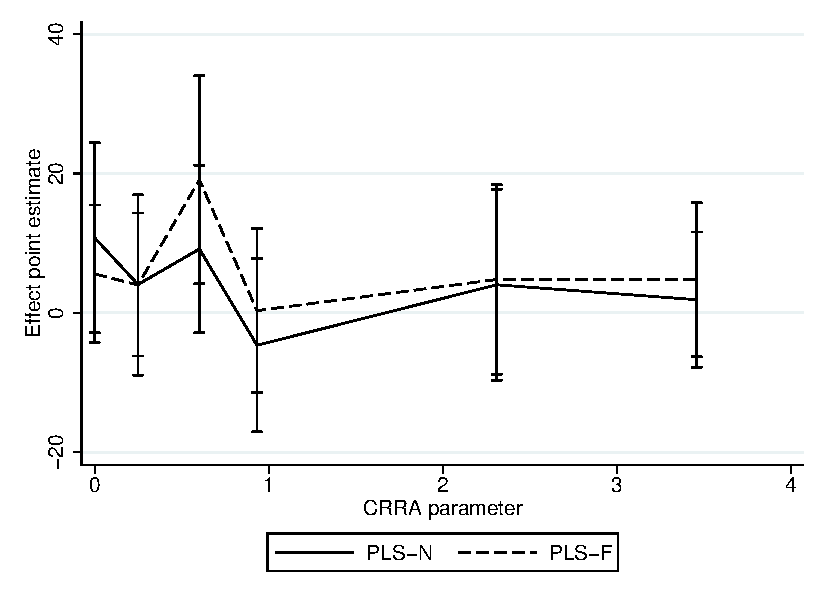
\includegraphics[width=\textwidth]{../../figures/line-mobile_totdepositsbyrisk.pdf}
		\end{figure}

	\clearpage

	\subsection{Savings behavior over project period}

        \begin{figure}[ht]
        \centering
        \caption{Timing of deposits}
        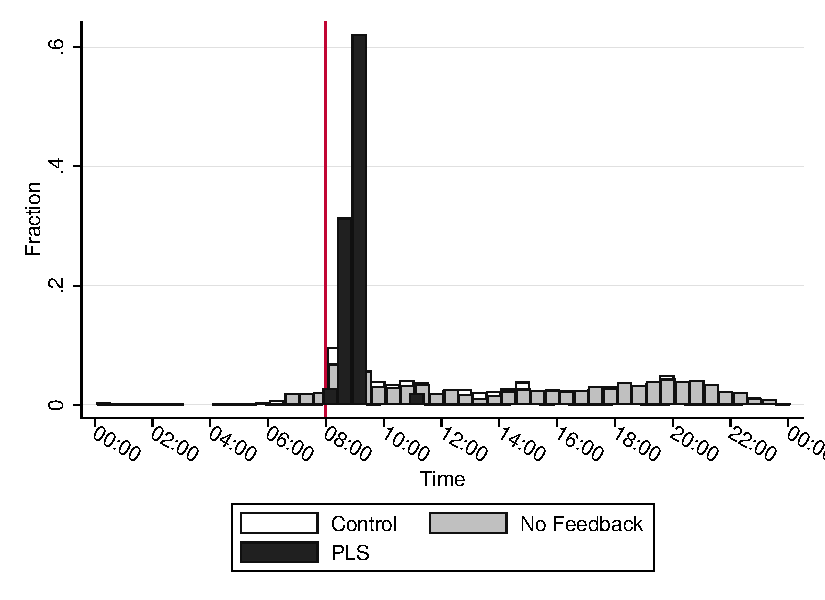
\includegraphics[width=\textwidth]{../../figures/hist-deposits.pdf}
        \caption*{\footnotesize \emph{Notes:} This figure plots the empirical distribution of timing of all deposits over the project period. Each bin spans 30 minutes with a height equal to the fraction of all deposits within each treatment group. Participants received the first SMS at 8:00 that summarized how much the participant saved the previous day, how much the participant earned through a matching contribution or winnings, and their total balance. An hour later, participants received a second SMS encouraging them to save that day. Participants in \textsc{Regret} received a new lottery ticket with the second message.}
        \end{figure}

		\begin{figure}[ht]
		\centering
		\caption{Number of daily deposits}
		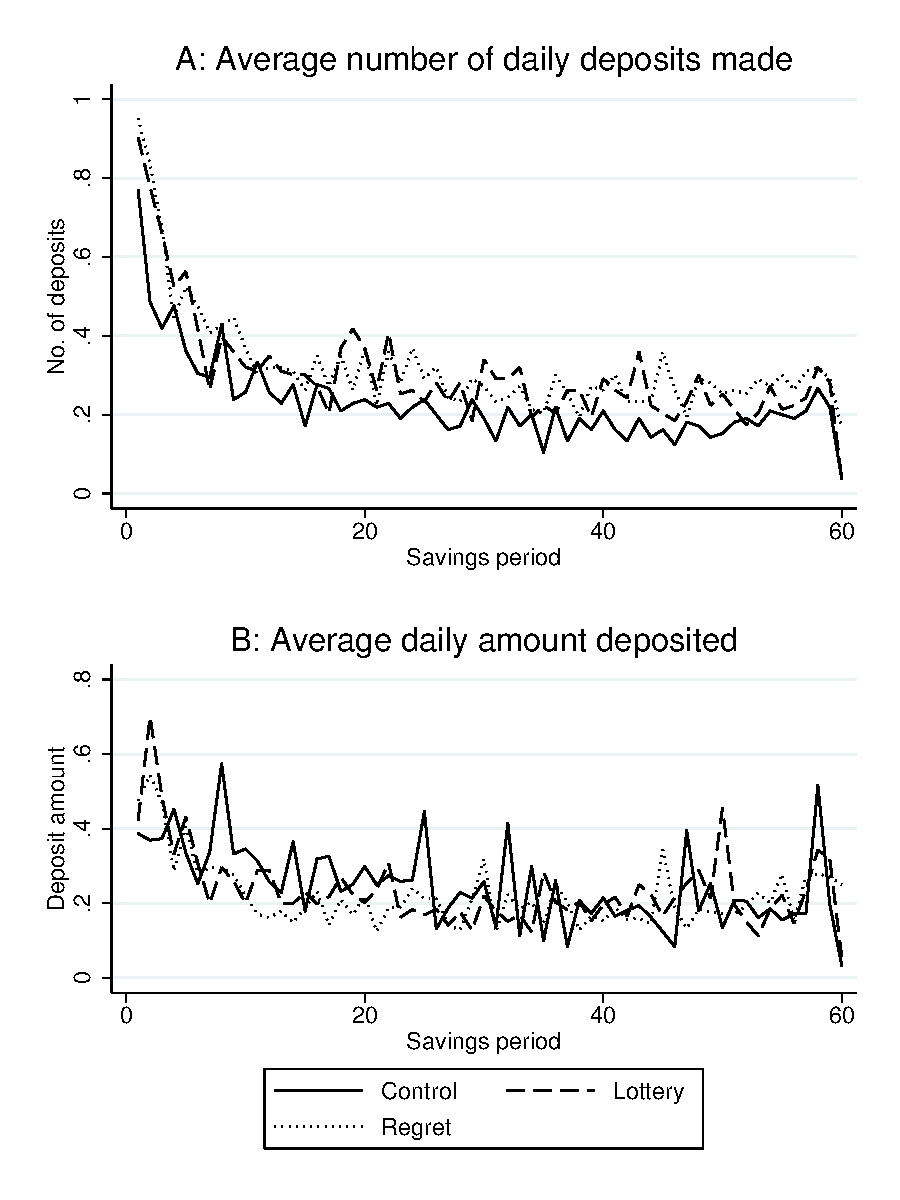
\includegraphics[width=\textwidth]{../../figures/line-deposits.pdf}
		\end{figure}

		\begin{figure}[ht]
		\centering
		\caption{Cumulative number of deposits}
		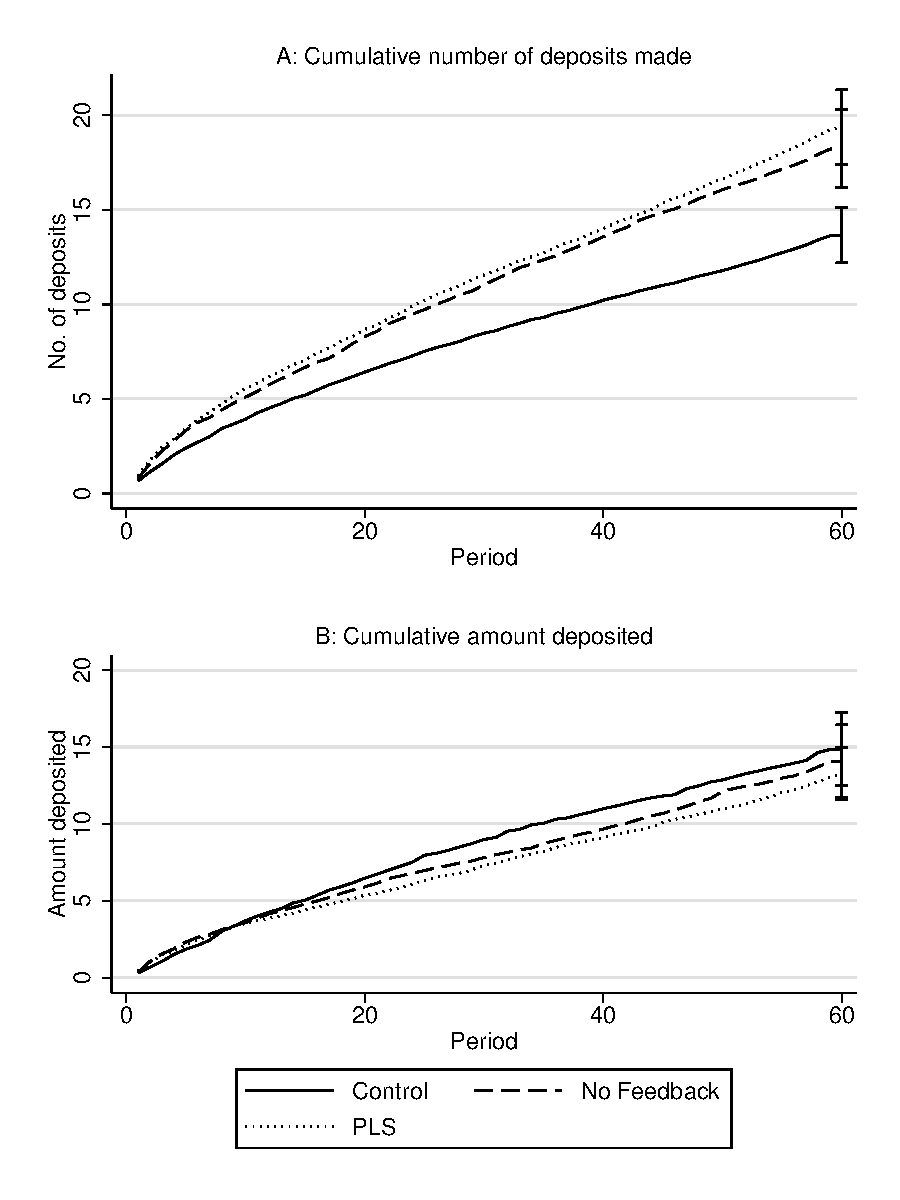
\includegraphics[width=\textwidth]{../../figures/line-cumdeposits.pdf}
		\end{figure}

		\begin{figure}[ht]
		\centering
		\caption{Daily balance averaged over all participants}
		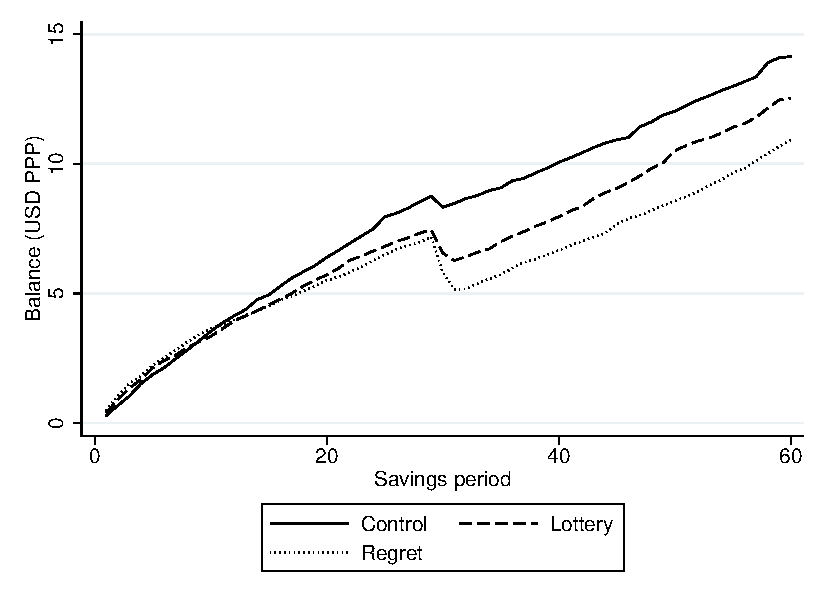
\includegraphics[width=\textwidth]{../../figures/line-balance.pdf}
		\end{figure}

	\clearpage

	\subsection{Panel treatment effects}

        \begin{figure}[ht]
        \centering
        \caption{Effects over time -- Number of deposits}
        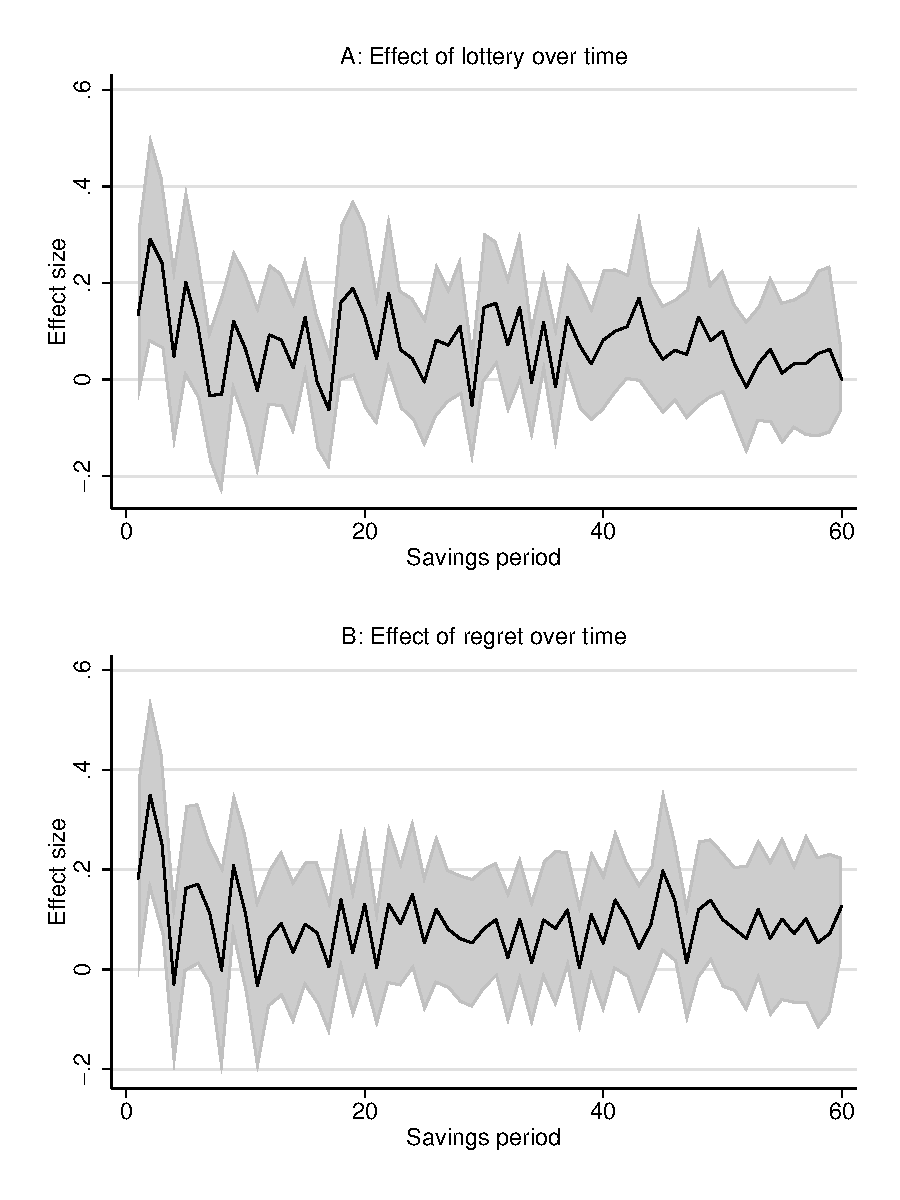
\includegraphics[width=\textwidth]{../../figures/line-timemobile_deposits.pdf}
        \end{figure}

        \begin{figure}[ht]
        \centering
        \caption{Effects over time -- Amount deposited}
        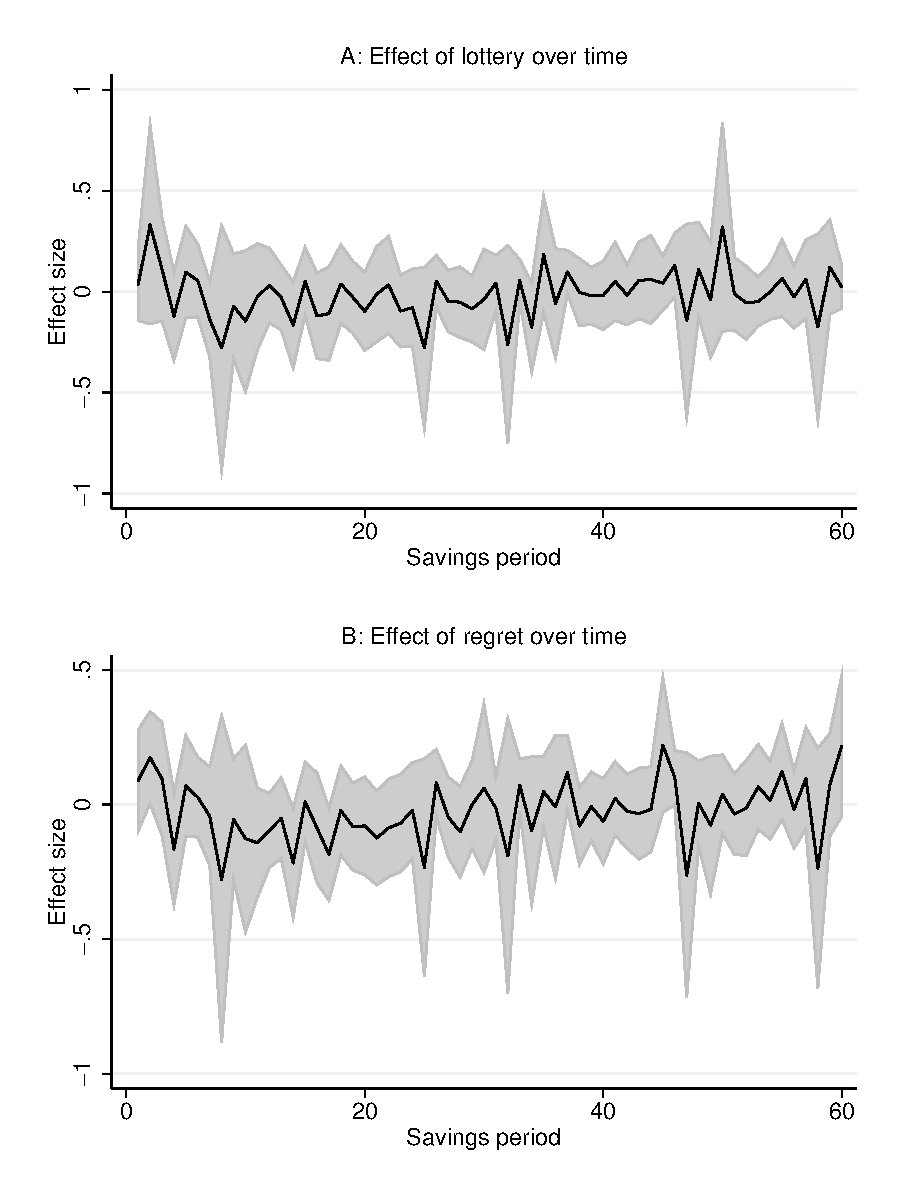
\includegraphics[width=\textwidth]{../../figures/line-timemobile_depositamount.pdf}
        \end{figure}

		% \begin{figure}[ht]
		% \centering
		% \caption{Autoregressive model - Saved on day t}
		% 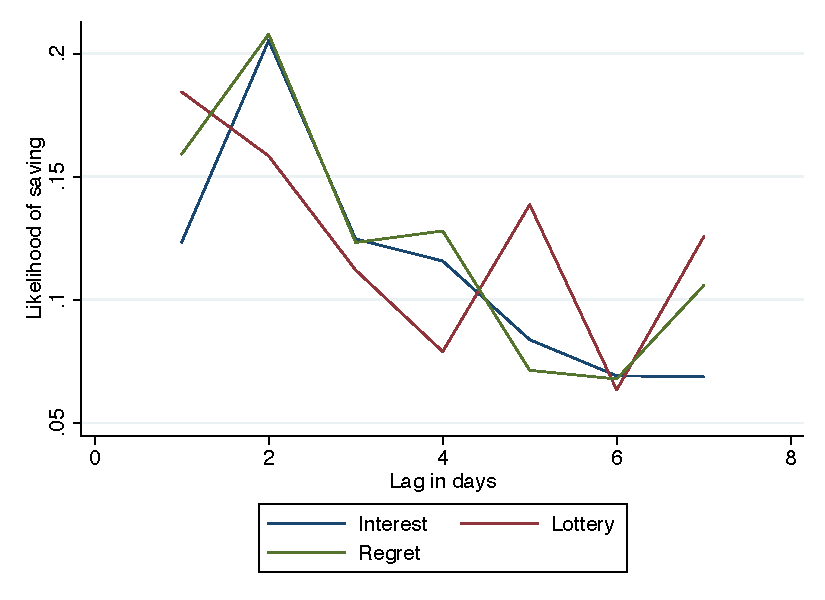
\includegraphics[width=\textwidth]{../../figures/line-ar.pdf}
		% \end{figure}
        %
		% \begin{figure}[ht]
		% \centering
		% \caption{Distributed lag model - Saved on day t}
		% 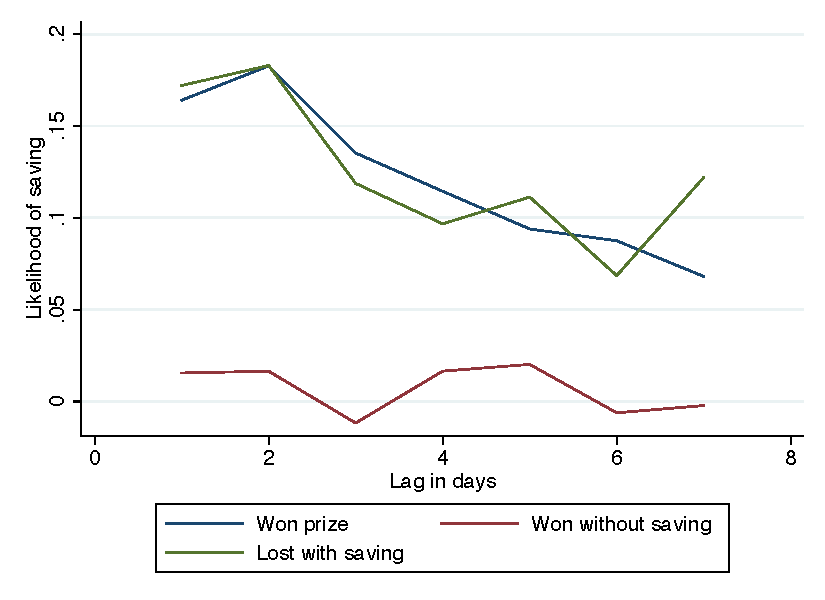
\includegraphics[width=\textwidth]{../../figures/line-dl.pdf}
		% \end{figure}

\end{document}
